%!TeX encoding = UTF-8
%!TEX program = xelatex
% ============================================================
% 《显微结构分析》课程作业
% 题目：单晶硅晶体学计算模板与 PDF 卡片的建立及带轴电子衍射模拟
% 结构：1 晶体学基础；2 Origin 模板与 PDF 卡片；3 计算晶体消光系数；4 带轴电子衍射模拟；5 结论
% 版式参照：X-Ray/课程论文模板（paper.tex）
% 编译：XeLaTeX 连续两遍；或运行本目录 complie.bat
% ============================================================
\documentclass[zihao=5,a4paper,twoside]{ctexart}

% ==================== 页面（同模板）====================
\usepackage[top=2.4cm,bottom=2.5cm,left=1.5cm,right=1.4cm,footskip=0.55cm]{geometry}

% ==================== 字体（同模板：中文楷体、数字 Times New Roman）====================
\setCJKmainfont{KaiTi}[AutoFakeBold=2.0]
\setmainfont{Times New Roman}
\usepackage{indentfirst}
\setlength{\parindent}{2em}
\setlength{\parskip}{0pt}
\raggedbottom

% ==================== 颜色（同模板）====================
\usepackage{xcolor}
\definecolor{secblue}{HTML}{365F91}
\definecolor{subblue}{HTML}{243F60}
\definecolor{bandblue}{HTML}{9CB8C7}

% ==================== 图表、数学、排版 ====================
\usepackage{graphicx}
\graphicspath{{assets/}}
\usepackage{float}
\usepackage{placeins}
\usepackage{booktabs}
\usepackage{array}
\usepackage{makecell}
\usepackage{amsmath,amssymb}
\usepackage{bm}
\usepackage{caption}
\usepackage[labelfont=bf]{subcaption}
\usepackage{enumitem}
\usepackage{tikz}
\usepackage{listings}
\usepackage[hidelinks]{hyperref}

% ==================== 编号（按节编号，如 图 2-5）====================
\numberwithin{figure}{section}
\numberwithin{table}{section}
\numberwithin{equation}{section}
\renewcommand{\thefigure}{\thesection-\arabic{figure}}
\renewcommand{\thetable}{\thesection-\arabic{table}}
\renewcommand{\theequation}{\thesection-\arabic{equation}}

\captionsetup{font=small,labelfont=bf,labelsep=quad}
\captionsetup[subfigure]{font=footnotesize,labelfont=bf,labelsep=space}

% ==================== 标题样式（同模板：楷体、蓝色层级）====================
\ctexset{
  section = {
    format     = {\color{secblue}\bfseries\fontsize{13pt}{16pt}\selectfont},
    number     = {\thesection.},
    aftername  = {\hspace{0.4em}},
    beforeskip = 15pt plus 3pt minus 2pt,
    afterskip  = 7pt plus 2pt,
  },
  subsection = {
    format     = {\color{secblue}\bfseries\fontsize{12pt}{15pt}\selectfont},
    aftername  = {\hspace{0.4em}},
    beforeskip = 12pt plus 2pt,
    afterskip  = 5pt plus 1pt,
  },
  subsubsection = {
    format     = {\color{subblue}\bfseries\fontsize{11pt}{14pt}\selectfont},
    aftername  = {\hspace{0.4em}},
    beforeskip = 10pt plus 2pt,
    afterskip  = 4pt plus 1pt,
  },
}

% ==================== 代码/公式清单样式 ====================
\lstset{
  basicstyle=\ttfamily\footnotesize,
  breaklines=true,
  columns=fullflexible,
  keepspaces=true,
  showstringspaces=false,
  frame=single,
  rulecolor=\color{gray!45},
  backgroundcolor=\color{gray!5},
  aboveskip=4pt,
  belowskip=4pt,
  xleftmargin=0.4em,
  xrightmargin=0.4em,
}

% ==================== 页脚（同模板）====================
\usepackage{fancyhdr}
\pagestyle{fancy}
\fancyhf{}
\renewcommand{\headrulewidth}{0pt}
\fancyfoot[RO]{\fontsize{8pt}{10pt}\selectfont |\enspace\thepage}
\fancyfoot[LE]{\fontsize{8pt}{10pt}\selectfont \thepage\enspace|}
\fancypagestyle{plain}{%
  \fancyhf{}%
  \renewcommand{\headrulewidth}{0pt}%
  \fancyfoot[RO]{\fontsize{8pt}{10pt}\selectfont |\enspace\thepage}%
}

\begin{document}
\linespread{1.3}\selectfont

% ==================== 首页题头 ====================
\hspace*{0.25cm}%
\begin{minipage}[c]{15.75cm}
  \setlength{\fboxsep}{0pt}%
  \colorbox{bandblue}{%
    \parbox[c][0.73cm][c]{15.75cm}{%
      \hspace{0.06cm}\textcolor{white}{\fontsize{16pt}{16pt}\selectfont\songti 《显微结构分析》课程作业}}}
\end{minipage}\hfill
\begin{minipage}[c]{1.4cm}
  \centering
\includegraphics[height=1.27cm]{logo/MUC.jpg}
\end{minipage}

\vspace{0.85cm}

% ==================== 题目与作者 ====================
{\centering\bfseries\fontsize{14pt}{20pt}\selectfont 单晶硅晶体学计算模板与 PDF 卡片的建立及带轴电子衍射模拟\par}

\vspace{0.55cm}

\hspace*{3.9cm}{\songti\fontsize{12pt}{16pt}\selectfont 刘佳鹏，24012639}

\vspace{0.45cm}

% ==================== 摘要与关键词 ====================
% ==================== 摘要 ====================
{\bfseries 摘要}\quad
以单晶硅（$a=b=c=5.43$~\AA，$\alpha=\beta=\gamma=90^\circ$）为例，在 Origin 中建立了一套可复用的晶体学计算模板：由晶格参数计算晶胞体积、倒易点阵参数、晶面间距、倒易矢量长度及晶面夹角，并据此构建了 Cu K$\alpha$ 条件下的单晶硅 PDF 卡片。把带轴电子衍射模拟分为两部分：先由 VESTA 导出的原子坐标和结构因子计算晶面的消光系数，判断哪些反射允许、哪些消光；再以 [001]、[111]、[332]、[334]、[345] 五个带轴为例，用晶带方程建立二维倒易点阵，计算衍射点坐标，并用散点图和三维 Waterfall 图绘制衍射图。结果表明，模拟图谱的对称性与点阵几何符合立方金刚石结构的预期，110 等反射因结构因子为零而消光。

\vspace{4pt}

\par\noindent{\heiti 关键词：}晶体学计算；Origin；PDF 卡片；电子衍射；单晶硅；结构因子


% ==================== 正文 ====================
% ==================== 1 晶体学与电子衍射基础 ====================
\section{晶体学与电子衍射基础}

\subsection{晶胞参数、晶胞体积与倒易点阵}

描述一个晶胞需要六个参数：三条棱长 $a,b,c$ 和三个夹角 $\alpha,\beta,\gamma$。晶胞体积为
\begin{equation}
V=abc\sqrt{1-\cos^2\alpha-\cos^2\beta-\cos^2\gamma+2\cos\alpha\cos\beta\cos\gamma}.
\label{eq:volume}
\end{equation}
倒易点阵基矢 $\bm{a}^*,\bm{b}^*,\bm{c}^*$ 由实空间基矢 $\bm{a},\bm{b},\bm{c}$ 定义：
\begin{equation}
\bm{a}^*=\frac{\bm{b}\times\bm{c}}{\bm{a}\cdot(\bm{b}\times\bm{c})},\qquad
\bm{b}^*=\frac{\bm{c}\times\bm{a}}{\bm{a}\cdot(\bm{b}\times\bm{c})},\qquad
\bm{c}^*=\frac{\bm{a}\times\bm{b}}{\bm{a}\cdot(\bm{b}\times\bm{c})}.
\label{eq:reciprocal-vectors}
\end{equation}
在晶体学中通常不写固体物理中的 $2\pi$ 因子，因此 $|\bm{a}^*|=1/d_{100}$，即倒易基矢的长度等于同名晶面间距的倒数。倒易点阵的六个参数可用实空间参数表示为
\begin{equation}
a^*=\frac{bc\sin\alpha}{V},\qquad
b^*=\frac{ac\sin\beta}{V},\qquad
c^*=\frac{ab\sin\gamma}{V},
\label{eq:reciprocal-lengths}
\end{equation}
\begin{equation}
\cos\alpha^*=\frac{\cos\beta\cos\gamma-\cos\alpha}{\sin\beta\sin\gamma},\quad
\cos\beta^*=\frac{\cos\alpha\cos\gamma-\cos\beta}{\sin\alpha\sin\gamma},\quad
\cos\gamma^*=\frac{\cos\alpha\cos\beta-\cos\gamma}{\sin\alpha\sin\beta}.
\label{eq:reciprocal-angles}
\end{equation}
对立方晶系，$a=b=c$、$\alpha=\beta=\gamma=90^\circ$，于是
\begin{equation}
V=a^3,\qquad a^*=b^*=c^*=\frac{1}{a},\qquad \alpha^*=\beta^*=\gamma^*=90^\circ.
\label{eq:cubic-reciprocal}
\end{equation}

\subsection{晶面间距、倒易矢量长度与晶面夹角}

晶面 $(hkl)$ 的法向平行于同名倒易矢量 $\bm{G}_{hkl}=h\bm{a}^*+k\bm{b}^*+l\bm{c}^*$，晶面间距等于该倒易矢量长度的倒数：
\begin{equation}
\frac{1}{d_{hkl}^2}=h^2a^{*2}+k^2b^{*2}+l^2c^{*2}
+2hka^*b^*\cos\gamma^*+2hla^*c^*\cos\beta^*+2klb^*c^*\cos\alpha^*.
\label{eq:dspacing}
\end{equation}
对立方晶系，式 \eqref{eq:dspacing} 简化为
\begin{equation}
d_{hkl}=\frac{a}{\sqrt{h^2+k^2+l^2}}.
\label{eq:dspacing-cubic}
\end{equation}
两个倒易矢量 $\bm{G}_1=(h_1k_1l_1)^*$、$\bm{G}_2=(h_2k_2l_2)^*$ 的长度为
\begin{equation}
r_i=\left|\bm{G}_i\right|=\sqrt{h_i^2a^{*2}+k_i^2b^{*2}+l_i^2c^{*2}
+2h_ik_ia^*b^*\cos\gamma^*+2h_il_ia^*c^*\cos\beta^*+2k_il_ib^*c^*\cos\alpha^*},
\quad i=1,2.
\label{eq:rlength}
\end{equation}
二者之间的夹角 $\theta$ 满足
\begin{equation}
\cos\theta=\frac{\bm{G}_1\cdot\bm{G}_2}{r_1r_2}
=\frac{1}{r_1r_2}\left[
\begin{aligned}
&h_1h_2a^{*2}+k_1k_2b^{*2}+l_1l_2c^{*2}\\
&+(k_1l_2+k_2l_1)b^*c^*\cos\alpha^*
 +(l_1h_2+l_2h_1)c^*a^*\cos\beta^*\\
&+(h_1k_2+h_2k_1)a^*b^*\cos\gamma^*
\end{aligned}
\right].
\label{eq:angle}
\end{equation}
式 \eqref{eq:rlength} 和式 \eqref{eq:angle} 就是 Origin 计算模板中 $r_1$、$r_2$ 和 $\theta$ 三列的计算依据。

\subsection{晶带方程与带轴电子衍射}

相交于同一晶向的各晶面族构成一个晶带，该晶向称为晶带轴（zone axis），简称带轴，记为 $[uvw]$。晶面 $(hkl)$ 属于该晶带的条件是
\begin{equation}
hu+kv+lw=0.
\label{eq:zone-law}
\end{equation}
在倒易空间中，属于同一带轴的所有倒易点构成一个过原点的二维倒易面 $(uvw)^*$，带轴 $[uvw]$ 垂直于该面。带轴电子衍射花样就是三维倒易点阵沿该带轴方向的二维截面。由于电子波长很短（200~kV 时约 0.0251~\AA），Ewald 球半径很大，在零阶劳厄区（ZOLZ）内可以近似把倒易面看成与 Ewald 球相切的平面，因此能够同时观察到属于该带轴的大量衍射点。

若在二维倒易面内选取两条不共线的基矢 $\bm{g}_1=(h_1k_1l_1)^*$、$\bm{g}_2=(h_2k_2l_2)^*$，它们的长度分别为 $r_1$、$r_2$，夹角为 $\theta$，则任意格点可用整数 $m,n$ 表示为
\begin{equation}
\bm{g}=m\bm{g}_1+n\bm{g}_2.
\label{eq:2d-lattice}
\end{equation}
以 $\bm{g}_1$ 为 $x$ 轴，则该格点的二维坐标为
\begin{equation}
x=mr_1+nr_2\cos\theta,\qquad y=nr_2\sin\theta,
\label{eq:xy}
\end{equation}
对应的晶面指数为
\begin{equation}
h=mh_1+nh_2,\qquad k=mk_1+nk_2,\qquad l=ml_1+nl_2.
\label{eq:hkl-mn}
\end{equation}
式 \eqref{eq:xy} 和式 \eqref{eq:hkl-mn} 是第 4 章建立衍射图表格的核心。图 \ref{fig:reciprocal-plane} 给出了二维倒易面、基矢和带轴之间的几何关系。

\begin{figure}[H]
  \centering
  \begin{tikzpicture}[scale=1.15,>=stealth]
    \coordinate (O) at (0,0);
    \coordinate (G1) at (4.2,0);
    \coordinate (G2) at (1.6,2.45);
    \coordinate (G12) at (5.8,2.45);
    \draw[->,very thick,secblue] (O)--(G1) node[midway,below=3pt] {$\bm{g}_1$};
    \draw[->,very thick,secblue] (O)--(G2) node[midway,left=3pt] {$\bm{g}_2$};
    \draw[dashed,gray] (G1)--(G12)--(G2);
    \draw[->,very thick,red!70!black] (2.9,1.22)--(2.9,4.15)
      node[above] {$[uvw]\parallel(uvw)^*$};
    \fill (O) circle (1.7pt) node[below left] {000};
    \fill (G1) circle (1.7pt);
    \fill (G2) circle (1.7pt);
    \fill (G12) circle (1.7pt);
    \draw (0.8,0) arc (0:56.9:0.8) node[midway,right] {$\theta$};
    \node[gray] at (2.9,-0.8) {二维倒易面 $(uvw)^*$};
  \end{tikzpicture}
  \caption{带轴电子衍射的二维倒易面、基矢与带轴关系示意。$\bm{g}_1$、$\bm{g}_2$ 为面内基矢，$[uvw]$ 垂直于该倒易面；整数 $m,n$ 将基矢扩展到整个倒易面。}
  \label{fig:reciprocal-plane}
\end{figure}

\subsection{结构因子、消光规律与单晶硅结构}

衍射点的位置由倒易点阵决定，衍射点的强弱则由结构因子决定。晶胞内第 $j$ 个原子对 $(hkl)$ 反射的结构因子贡献为
\begin{equation}
F(hkl)=\sum_{j=1}^{N}g_jt_j(s)f_j(s)\exp\left[2\pi i(hx_j+ky_j+lz_j)\right],
\label{eq:structure-factor}
\end{equation}
其中 $g_j$ 为占有率，$t_j(s)$ 为温度因子，$f_j(s)$ 为原子散射因子，$(x_j,y_j,z_j)$ 为原子分数坐标。原子散射因子描述一个原子在给定方向上的散射振幅相对于一个自由电子散射振幅的比值（量纲为 1），随散射角增大而衰减；在 $s=\sin\theta/\lambda\to0$ 的前向散射极限下，$f(0)$ 近似等于该原子的核外电子数，即原子序数 $Z$。若近似取 $g_j=1$、$t_j=1$、$f_j=f$（常数），则
\begin{equation}
F(hkl)=f\sum_{j=1}^{N}\exp\left[2\pi i(hx_j+ky_j+lz_j)\right],\qquad I\propto|F|^2.
\label{eq:structure-factor-simple}
\end{equation}
本作业的 Origin 模板正是采用这一简化形式，并取 Si 的 $f=14$（Si 的原子序数 $Z=14$，即取前向散射极限值并忽略其随角度的衰减，详见第 \ref{sec:f14} 节）。

单晶硅为金刚石型立方结构，空间群 $Fd\bar{3}m$（No.~227），点阵常数 $a=5.43$~\AA，每个惯用晶胞含 8 个 Si 原子，其分数坐标列于表 \ref{tab:si-atoms}。该结构可看作两套面心立方点阵沿体对角线相对位移 $(1/4,1/4,1/4)$ 套构而成，每个 Si 原子与 4 个近邻形成正四面体配位，Si--Si 键长为 $\sqrt{3}a/4\approx2.35$~\AA。

\begin{table}[H]
  \centering
  \caption{单晶硅（$Fd\bar{3}m$，$a=5.43$~\AA）晶胞内 8 个 Si 原子的分数坐标}
  \label{tab:si-atoms}
  \small
  \begin{tabular}{cccc}
    \toprule
    序号 & $x$ & $y$ & $z$ \\
    \midrule
    1 & 0     & 0     & 0     \\
    2 & 0     & 1/2   & 1/2   \\
    3 & 1/2   & 0     & 1/2   \\
    4 & 1/2   & 1/2   & 0     \\
    5 & 1/4   & 1/4   & 1/4   \\
    6 & 1/4   & 3/4   & 3/4   \\
    7 & 3/4   & 1/4   & 3/4   \\
    8 & 3/4   & 3/4   & 1/4   \\
    \bottomrule
  \end{tabular}
\end{table}

把表 \ref{tab:si-atoms} 的坐标代入式 \eqref{eq:structure-factor-simple}，可得金刚石结构的结构因子
\begin{equation}
F=f\left[1+e^{\pi i(h+k)}+e^{\pi i(h+l)}+e^{\pi i(k+l)}\right]
\left[1+e^{\frac{\pi i}{2}(h+k+l)}\right].
\label{eq:diamond-F}
\end{equation}
由此得到金刚石结构的消光规律：
\begin{itemize}[leftmargin=2em,itemsep=1pt]
  \item $h,k,l$ 奇偶混合时，第一个方括号为 0，$F=0$；
  \item $h,k,l$ 全为偶数且 $h+k+l=4n+2$ 时，第二个方括号为 0，$F=0$；
  \item $h,k,l$ 全为奇数时，$|F|^2=32f^2$；
  \item $h,k,l$ 全为偶数且 $h+k+l=4n$ 时，$|F|^2=64f^2$。
\end{itemize}
因此，Si 的允许反射为 111、220、311、400、331、422、511/333、440 等，而 100、110、200、222、420、600 等消光。第 3 章将以 110 反射为例，用模板计算验证这一规律。

% ==================== 2 Origin 晶体学计算模板的建立 ====================
\section{Origin 晶体学计算模板的建立}

\subsection{工作簿、列结构与角度单位}

打开 Origin，新建一个工作簿，将其重命名为 \texttt{SIcalculator}，并新增 20 列，使工作表增加到 A--V 共 22 列，如图 \ref{fig:calc-setup}(a)(b) 所示。列数应与模板的列布局一致；后续如需增加计算项目，可在工作表中继续插入行或列。随后按“晶格参数—晶胞体积—倒易参数—晶面指数—结果”的顺序命名各列，如图 \ref{fig:calc-setup}(c) 和图 \ref{fig:calc-formula}(a) 所示。建议的列布局为：

\begin{itemize}[leftmargin=2em,itemsep=1pt]
  \item A--F：$a,b,c,\alpha,\beta,\gamma$；
  \item G：晶胞体积 $V$；
  \item H--M：$a^*,b^*,c^*,\alpha^*,\beta^*,\gamma^*$；
  \item N--S：$h_1,k_1,l_1,h_2,k_2,l_2$；
  \item T--V：$r_1,r_2,\theta$。
\end{itemize}

\begin{figure}[H]
  \centering
  \begin{subfigure}[t]{0.40\linewidth}
    \centering
    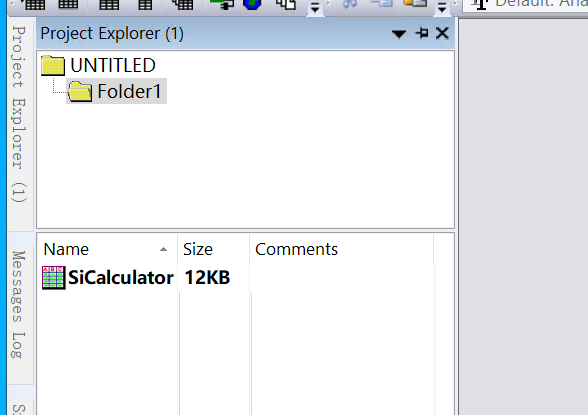
\includegraphics[width=\linewidth]{calc/c01.png}
    \caption{新建工作簿并命名为 \texttt{SIcalculator}}
    \label{fig:calc-setup-a}
  \end{subfigure}\hfill
  \begin{subfigure}[t]{0.30\linewidth}
    \centering
    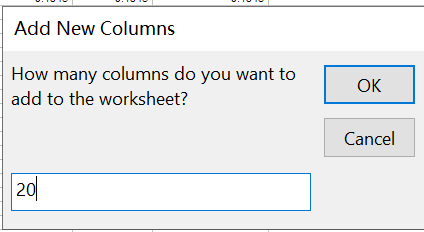
\includegraphics[width=\linewidth]{calc/c02.png}
    \caption{新增 20 列，增加到 A--V 共 22 列}
    \label{fig:calc-setup-b}
  \end{subfigure}

  \vspace{0.4em}
  \begin{subfigure}[t]{0.96\linewidth}
    \centering
    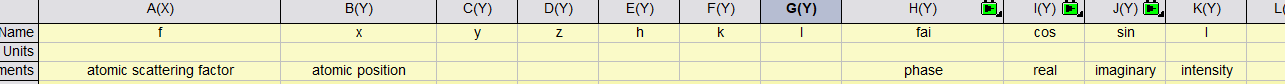
\includegraphics[width=\linewidth]{calc/c03.png}
    \caption{新建列并逐列命名}
    \label{fig:calc-setup-c}
  \end{subfigure}
  \caption{Origin 计算模板的初始设置：(a) 新建并重命名工作簿；(b) 新增 20 列，工作表增加到 A--V 共 22 列；(c) 建立列名。列名将直接作为公式中的变量名使用，因此命名应简洁且不重复。}
  \label{fig:calc-setup}
\end{figure}

需要特别强调角度单位。Origin 的三角函数默认可能使用弧度，而晶体学公式和日常输入都习惯使用角度制。应在 \texttt{Tools $\rightarrow$ Options}（或工作表属性）中把 Angular Unit 设为 Degree，如图 \ref{fig:calc-angle-volume}(a) 所示；否则式 \eqref{eq:volume} 和式 \eqref{eq:angle} 中的 \texttt{cos}、\texttt{acos} 会得到完全错误的结果。这一设置是本模板最容易出错、也最值得先检查的地方。

\begin{figure}[H]
  \centering
  \begin{subfigure}[t]{0.96\linewidth}
    \centering
    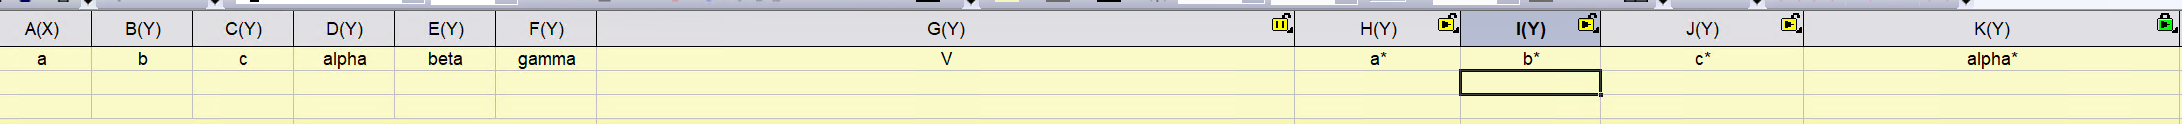
\includegraphics[width=\linewidth]{calc/c04.png}
    \caption{逐行检查并修正列名}
    \label{fig:calc-formula-a}
  \end{subfigure}

  \vspace{0.4em}
  \begin{subfigure}[t]{0.66\linewidth}
    \centering
    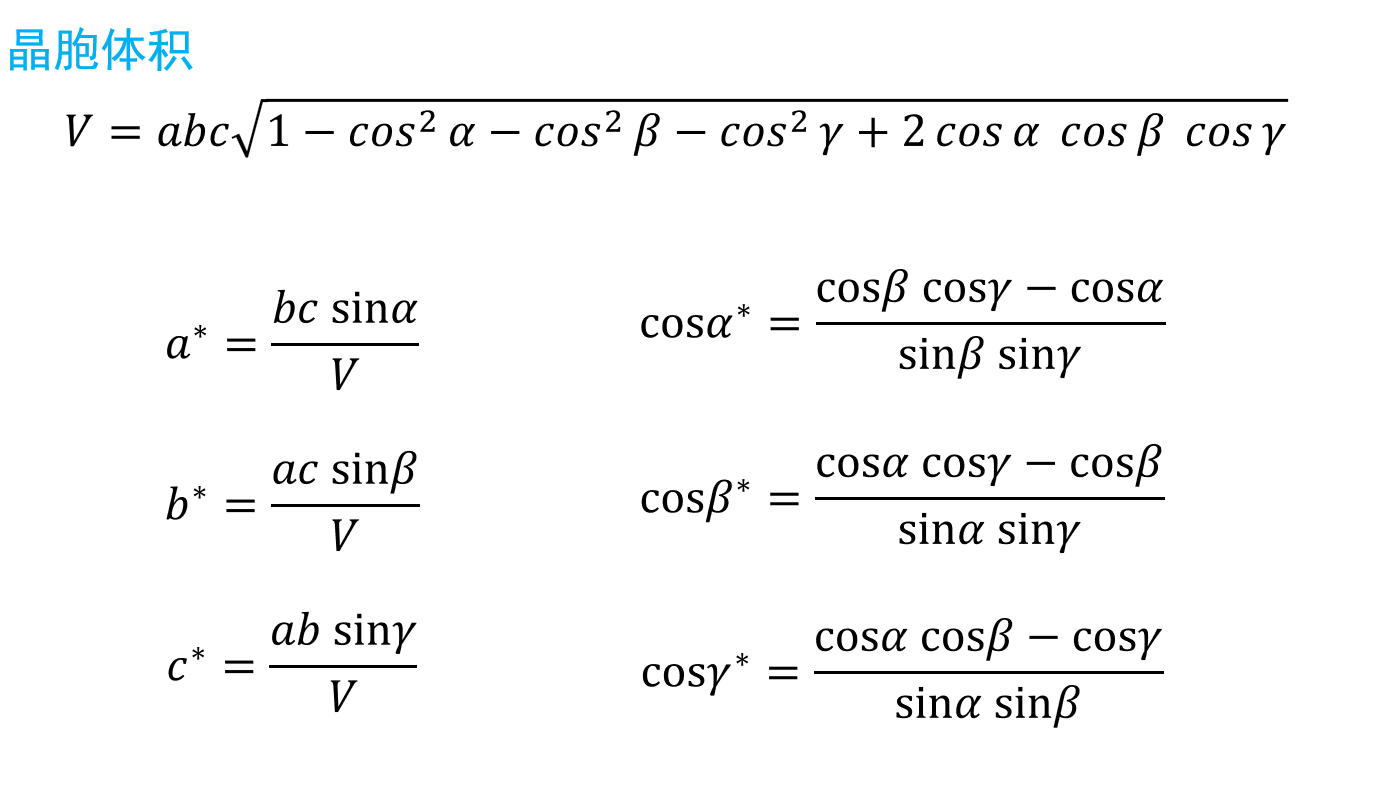
\includegraphics[width=\linewidth]{calc/c05.png}
    \caption{按公式表在对应列输入表达式}
    \label{fig:calc-formula-b}
  \end{subfigure}
  \caption{列名与公式输入。Origin 的公式可直接引用列名（如 \texttt{A}、\texttt{B}），也可引用列序号；使用列名更直观，但改名后公式中的引用必须同步修改。}
  \label{fig:calc-formula}
\end{figure}

\subsection{晶胞体积与倒易点阵参数}

在 A--F 列输入单晶硅的晶格参数：$a=b=c=5.43$，$\alpha=\beta=\gamma=90$，如图 \ref{fig:calc-angle-volume}(b) 所示。选中 G 列，按 \texttt{Ctrl+Q} 打开公式编辑框，输入式 \eqref{eq:volume} 对应的 Origin 表达式
\begin{lstlisting}
A*B*C*sqrt(1-cos(D)^2-cos(E)^2-cos(F)^2+2*cos(D)*cos(E)*cos(F))
\end{lstlisting}
按题目给定的 $a=5.43$~\AA，立方晶系中根号项严格等于 1，因此 $V=a^3=160.103$~\AA$^3$。图 \ref{fig:calc-volume-reciprocal}(a) 的界面数值为 159.22009~\AA$^3$，对应 $a=5.42$~\AA 的旧输入；它恰好说明模板会随 A--C 列的输入而变化，正式计算前应先把晶格参数核对到题目给定值。若体积与 $a^3$ 出现明显偏差，应首先检查角度单位是否误设为弧度。

倒易参数 H--M 列分别输入
\begin{lstlisting}
B*C*sin(D)/G
A*C*sin(E)/G
A*B*sin(F)/G
acos((cos(E)*cos(F)-cos(D))/(sin(E)*sin(F)))
acos((cos(D)*cos(F)-cos(E))/(sin(D)*sin(F)))
acos((cos(E)*cos(D)-cos(F))/(sin(E)*sin(D)))
\end{lstlisting}
其中 H、I、J 三列为 $a^*,b^*,c^*$，K、L、M 三列为 $\alpha^*,\beta^*,\gamma^*$。对单晶硅，模板给出 $a^*=b^*=c^*=0.18416$~\AA$^{-1}$，$\alpha^*=\beta^*=\gamma^*=90^\circ$，如图 \ref{fig:calc-volume-reciprocal}(b) 所示。这与式 \eqref{eq:cubic-reciprocal} 的解析结果一致，可作为模板正确性的第一个自检。

\begin{figure}[H]
  \centering
  \begin{subfigure}[t]{0.32\linewidth}
    \centering
    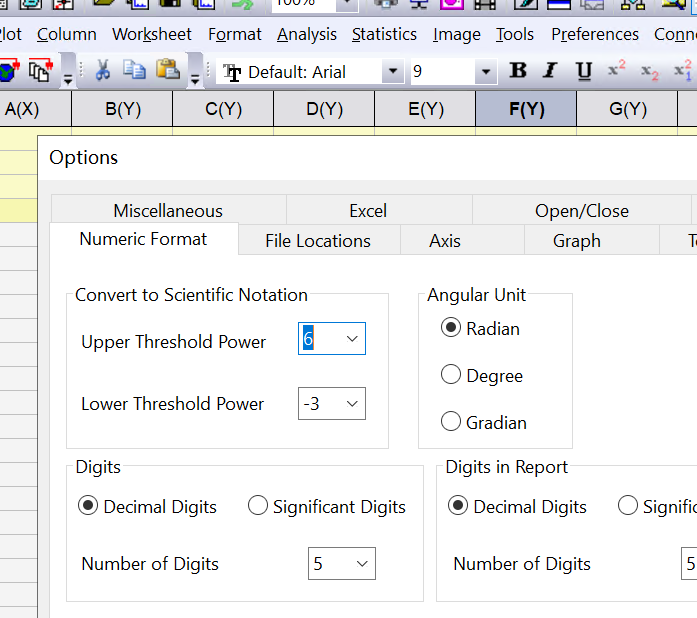
\includegraphics[width=\linewidth]{calc/c06.png}
    \caption{把角度单位设为度}
    \label{fig:calc-angle-volume-a}
  \end{subfigure}\hfill
  \begin{subfigure}[t]{0.12\linewidth}
    \centering
    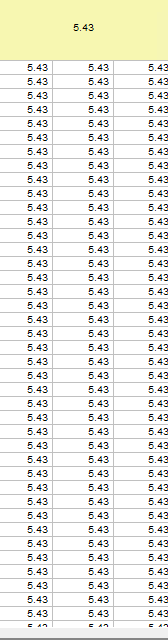
\includegraphics[height=5.4cm]{calc/c07.png}
    \caption{输入 $a,b,c$}
    \label{fig:calc-angle-volume-b}
  \end{subfigure}\hfill
  \begin{subfigure}[t]{0.50\linewidth}
    \centering
    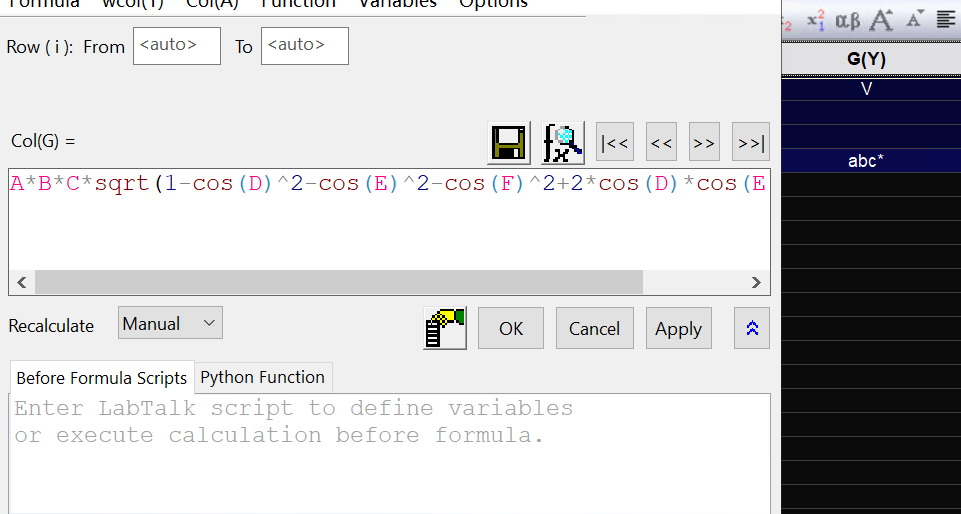
\includegraphics[width=\linewidth]{calc/c08.png}
    \caption{输入体积公式}
    \label{fig:calc-angle-volume-c}
  \end{subfigure}
  \caption{角度单位、晶格参数与体积公式：(a) 将角度单位设为 Degree；(b) 在 A--C 列输入 5.43；(c) 在 G 列输入体积公式。}
  \label{fig:calc-angle-volume}
\end{figure}

\begin{figure}[H]
  \centering
  \begin{subfigure}[t]{0.42\linewidth}
    \centering
    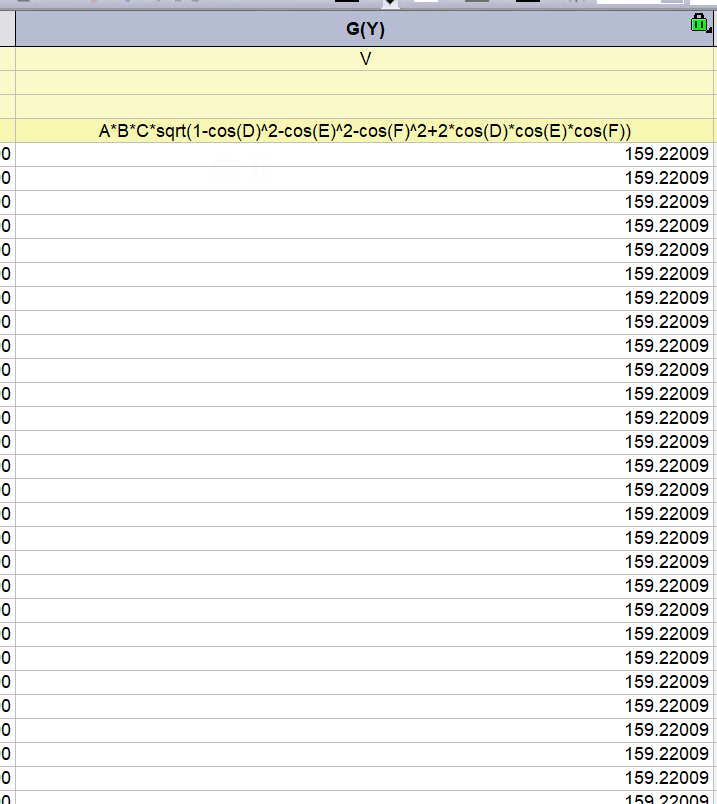
\includegraphics[width=\linewidth]{calc/c09.png}
    \caption{体积计算结果（界面示例；该截图的 159.22009~\AA$^3$ 对应 $a=5.42$~\AA，按题目 $a=5.43$~\AA 计算为 160.103~\AA$^3$）}
    \label{fig:calc-volume-reciprocal-a}
  \end{subfigure}\hfill
  \begin{subfigure}[t]{0.52\linewidth}
    \centering
    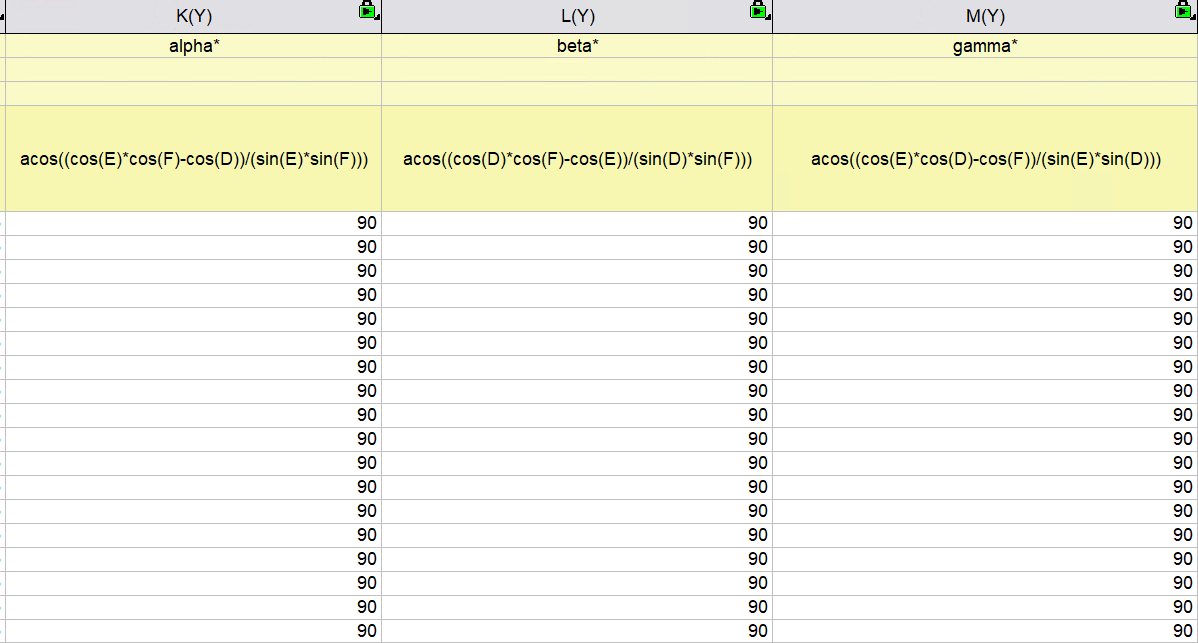
\includegraphics[width=\linewidth]{calc/c10.png}
    \caption{倒易点阵参数与倒易夹角}
    \label{fig:calc-volume-reciprocal-b}
  \end{subfigure}
  \caption{体积与倒易参数的计算结果。立方晶系中 $a^*=b^*=c^*=1/a=0.18416$~\AA$^{-1}$，$\alpha^*=\beta^*=\gamma^*=90^\circ$。}
  \label{fig:calc-volume-reciprocal}
\end{figure}

\subsection{晶面间距、倒易矢量长度与晶面夹角}

在 N--S 列输入两组晶面指数 $h_1k_1l_1$ 和 $h_2k_2l_2$，然后在 T、U、V 三列分别输入
\begin{lstlisting}
SQRT((N*H)^2+(O*I)^2+(P*J)^2+2*N*O*H*I*cos(M)+2*N*P*H*J*cos(L)+2*O*P*I*J*cos(K))
SQRT((Q*H)^2+(R*I)^2+(S*J)^2+2*Q*R*H*I*cos(M)+2*Q*S*H*J*cos(L)+2*R*S*I*J*cos(K))
ACOS((N*Q*H^2+O*R*I^2+P*S*J^2+(N*R+O*Q)*H*I*cos(M)+(N*S+P*Q)*H*J*cos(L)+(O*S+P*R)*I*J*cos(K))/(T*U))
\end{lstlisting}
其中 T、U 分别为 $r_1=1/d_1$、$r_2=1/d_2$，V 为两倒易矢量（即两晶面法向）之间的夹角 $\theta$。图 \ref{fig:calc-rtheta}(a)(b) 给出了输入界面与计算结果；改变 N--S 列的指数，T--V 列会自动更新，因此同一个模板可以反复用于不同的晶面组合。

以 $(h_1k_1l_1)=(423)$、$(h_2k_2l_2)=(232)$ 为例，在 N--S 列输入 4、2、3、2、3、2，T--V 列立即给出对应的 $r_1$、$r_2$ 和 $\theta$。这两个晶面只是任意选取的一组示例，并不对应本作业要求的五个带轴；若要计算某一带轴的基矢，应先按式 \eqref{eq:zone-law} 选取满足 $hu+kv+lw=0$ 的两条反射，具体做法见第 4 章。对立方晶系，也可以直接用解析式校验模板：
\begin{equation}
r_{hkl}=\frac{\sqrt{h^2+k^2+l^2}}{a},\qquad
\cos\theta=\frac{h_1h_2+k_1k_2+l_1l_2}{\sqrt{h_1^2+k_1^2+l_1^2}\sqrt{h_2^2+k_2^2+l_2^2}}.
\label{eq:cubic-check}
\end{equation}

\begin{figure}[H]
  \centering
  \begin{subfigure}[t]{0.22\linewidth}
    \centering
    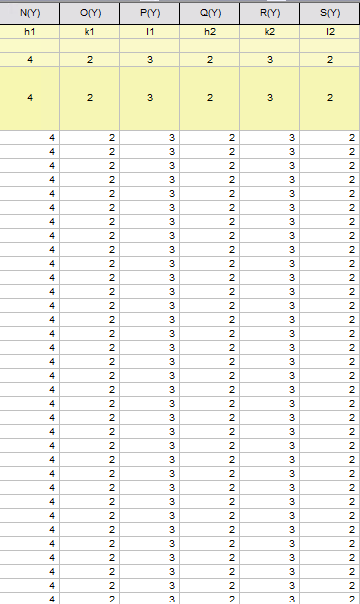
\includegraphics[width=\linewidth]{calc/c11.png}
    \caption{输入两组晶面指数}
    \label{fig:calc-rtheta-a}
  \end{subfigure}\hfill
  \begin{subfigure}[t]{0.70\linewidth}
    \centering
    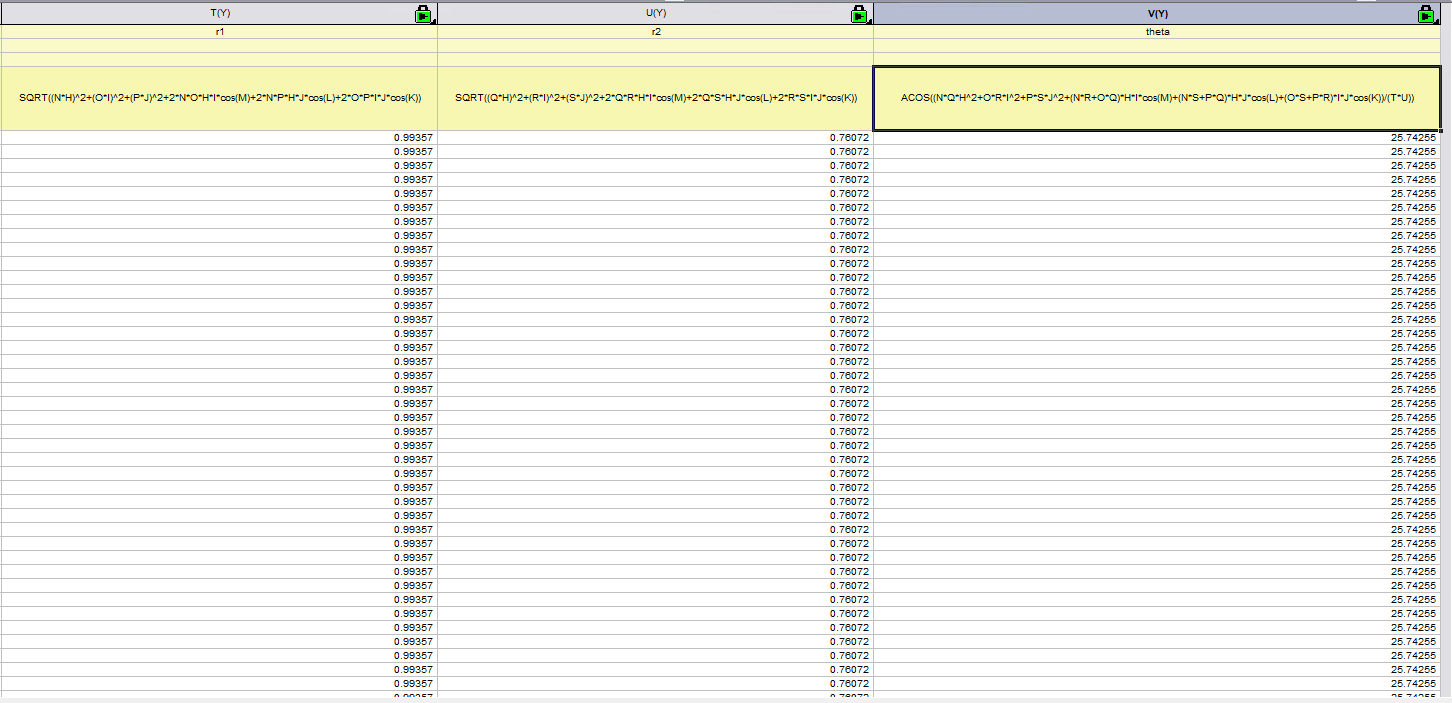
\includegraphics[width=\linewidth]{calc/c12.png}
    \caption{$r_1$、$r_2$ 与 $\theta$ 的计算结果}
    \label{fig:calc-rtheta-b}
  \end{subfigure}
  \caption{晶面组合的输入与 $r_1$、$r_2$、$\theta$ 的计算。T、U、V 三列分别对应式 \eqref{eq:rlength} 和式 \eqref{eq:angle}。}
  \label{fig:calc-rtheta}
\end{figure}

\subsection{单晶硅 PDF 卡片的构建}
\label{sec:cromer-mann}

PDF 卡片的核心信息是每一组衍射线的晶面指数 $hkl$、晶面间距 $d$、衍射角 $2\theta$ 和相对强度 $I/I_0$。在已建立的模板后面继续增加四列：$2\theta$、多重性 $N_{hkl}$、$|F_{hkl}|^2$ 和 $I/I_0$，即可把“晶体学计算器”扩展为“PDF 卡片生成器”；若需比较原子散射因子的影响，可再加一列 $I/I_0(f(s))$。

由 Bragg 方程 $2d\sin\theta=\lambda$ 得
\begin{equation}
2\theta=2\arcsin\left(\frac{\lambda}{2d_{hkl}}\right).
\label{eq:bragg}
\end{equation}
本作业取 Cu K$\alpha_1$ 波长 $\lambda=1.5406$~\AA。对粉末衍射，某一组 $\{hkl\}$ 的相对强度还正比于多重性 $N_{hkl}$ 和 Lorentz-偏振因子 $LP$：
\begin{equation}
I_{hkl}\propto N_{hkl}|F_{hkl}|^2LP,\qquad
LP=\frac{1+\cos^2 2\theta}{\sin^2\theta\cos\theta}.
\label{eq:intensity-powder}
\end{equation}
其中 $N_{hkl}$ 是同一 $d$ 值下等价晶面（包括交换和正负号）的数目。把表 \ref{tab:si-atoms} 的 8 个原子坐标代入式 \eqref{eq:structure-factor-simple}，即可得到 $|F_{hkl}|^2$；再用式 \eqref{eq:bragg} 和式 \eqref{eq:intensity-powder} 即可得到 $2\theta$ 和相对强度。表 \ref{tab:pdf-card} 列出了单晶硅的主要 PDF 卡片数据。

\begin{table}[H]
  \centering
  \caption{由计算模板得到的单晶硅 PDF 卡片数据（Cu K$\alpha_1$，$\lambda=1.5406$~\AA）}
  \label{tab:pdf-card}
  \small
  \setlength{\tabcolsep}{3pt}
  \renewcommand{\arraystretch}{1.05}
  \begin{tabular}{ccccccc}
    \toprule
    $hkl$ & $d$/\AA & $2\theta$/$^\circ$ & 多重性 & $|F|^2$ & $I/I_0$ ($f=14$) & $I/I_0$ ($f(s)$, $B=0.5$~\AA$^2$) \\
    \midrule
    111 & 3.1350 & 28.45 & 8  & 6272  & 100.0 & 100.0 \\
    220 & 1.9198 & 47.31 & 12 & 12544 & 98.0  & 64.3  \\
    311 & 1.6372 & 56.13 & 24 & 6272  & 66.4  & 37.3  \\
    400 & 1.3575 & 69.14 & 6  & 12544 & 21.0  & 9.6   \\
    331 & 1.2457 & 76.39 & 24 & 6272  & 34.8  & 14.1  \\
    422 & 1.1084 & 88.05 & 24 & 12544 & 57.1  & 19.4  \\
    511/333 & 1.0450 & 94.97 & 32 & 6272 & 36.2 & 11.1 \\
    440 & 0.9599 & 106.74 & 12 & 12544 & 27.9 & 7.2  \\
    531 & 0.9178 & 114.12 & 48 & 6272 & 60.3 & 14.0  \\
    620 & 0.8586 & 127.59 & 24 & 12544 & 76.4 & 15.1 \\
    533 & 0.8281 & 136.94 & 24 & 6272 & 47.8 & 8.6  \\
    444 & 0.7838 & 158.74 & 8  & 12544 & 69.2 & 10.6 \\
    \bottomrule
  \end{tabular}
\end{table}

表 \ref{tab:pdf-card} 中前一个强度列取 $f=14$，与第 3 章结构因子/消光系数计算的简化模型一致——$f$ 为原子散射因子，$14$ 即 Si 的原子序数，相当于只保留其前向散射值、忽略随角度的衰减（其含义与适用范围见第 \ref{sec:f14} 节）；后一个强度列把常数 $f$ 换成 Si 的 Cromer--Mann 原子散射因子 $f(s)$，并取温度因子 $B=0.5$~\AA$^2$，即
\begin{equation}
f(s)=\sum_{i=1}^{4}a_i e^{-b_i s^2}+c,\qquad s=\frac{\sin\theta}{\lambda}=\frac{1}{2d},
\label{eq:cromer-mann}
\end{equation}
其中 $a_1=6.2915$、$b_1=2.4386$，$a_2=3.0353$、$b_2=32.3337$，$a_3=1.9891$、$b_3=0.6785$，$a_4=1.5410$、$b_4=81.6937$，$c=1.1407$。$f(0)\approx14$，正好等于 Si 的原子序数，可作为系数是否抄对的检查。

表 \ref{tab:pdf-card} 与图 \ref{fig:pdf-card} 的数值由同一套公式算出，但作图方式不同：表格数据来自第 2.1--2.4 节的 Origin 模板（逐列输入晶格参数、$2\theta$、多重性和强度公式），而图 \ref{fig:pdf-card} 的棒图是用 \textbf{Python 3 + matplotlib} 编写的脚本自动生成的，没有在 Origin 中手工绘制。脚本的基本做法是：固定晶格常数、波长、常数 $f$ 和温度因子后，遍历 $0\le l\le k\le h\le 8$ 的 $hkl$，用式 \eqref{eq:structure-factor-simple} 求 $|F|^2$（为零即判为消光并剔除），用式 \eqref{eq:bragg} 求 $2\theta$、用式 \eqref{eq:intensity-powder} 求相对强度，按 $d$ 把退化组合（如 333 与 511）合并，归一化后用 \texttt{vlines} 画出两组棒图。

之所以用脚本而不是手工绘图，原因有三点：其一，PDF 卡片需要对上百个 $hkl$ 逐一枚举、按 $d$ 分组并统计多重性，手工录入既慢又容易漏项；其二，同一批数据要同时给出 $f=14$ 与 $f(s)$ 两套强度并排比较，脚本只需改一行常数即可重绘；其三，脚本可以同步打印表 \ref{tab:pdf-card} 的每一行，与 Origin 模板的结果逐行对照，起到交叉校验的作用（两者数值完全一致）。完整的构建思路、代码和运行方法见附录 C。若希望全部在 Origin 内完成，也可以把表 \ref{tab:pdf-card} 的 $2\theta$ 与强度两列直接画成柱状或棒状图，但枚举、分组和多重性统计仍建议由代码完成。

\begin{figure}[H]
  \centering
  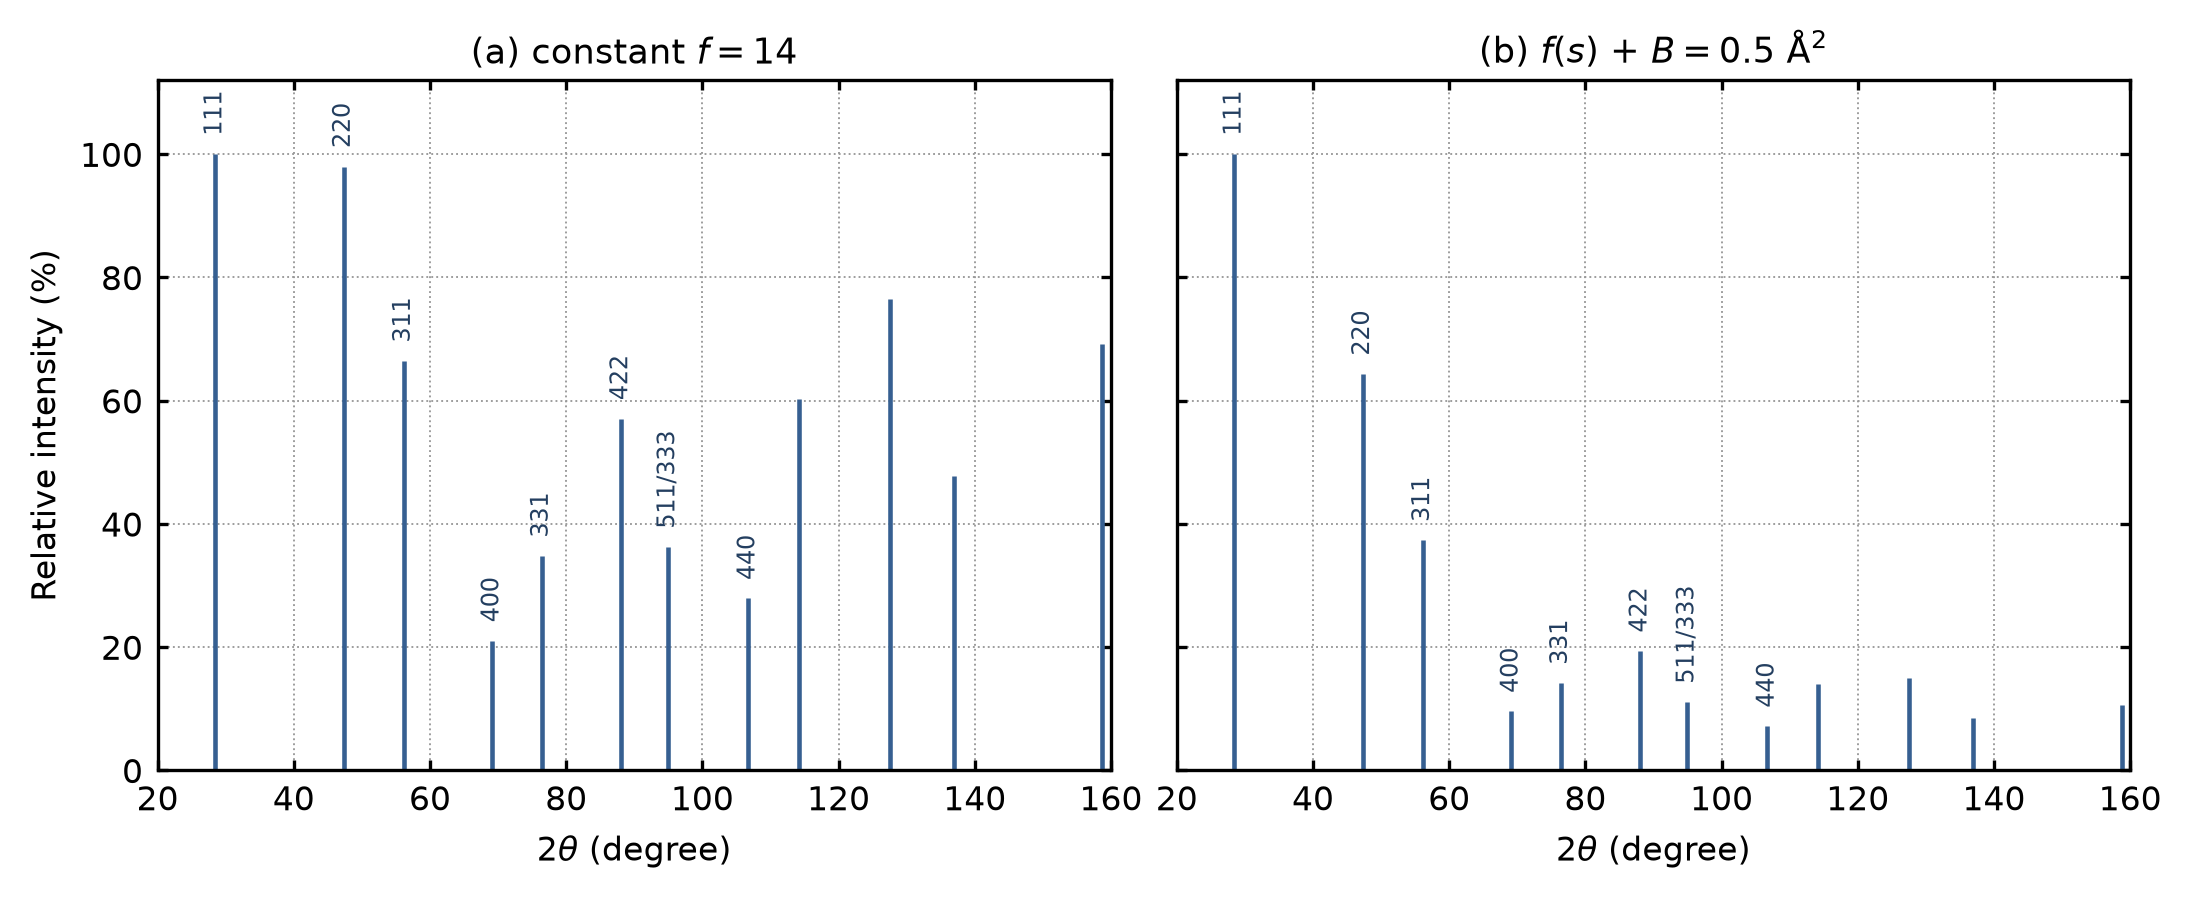
\includegraphics[width=\linewidth]{pdfcard.png}
  \caption{由计算模板得到的单晶硅 PDF 卡片棒图（Cu K$\alpha_1$）：(a) 常数原子散射因子 $f=14$；(b) 采用 Si 的 $f(s)$ 并取 $B=0.5$~\AA$^2$。两图的峰位完全相同，但高角反射的相对强度在后一模型中明显减弱。}
  \label{fig:pdf-card}
\end{figure}

从图 \ref{fig:pdf-card} 和表 \ref{tab:pdf-card} 可以看出：单晶硅最强的衍射线是 111，其次是 220、311、422 等；高角反射（如 531、620、444）在 $f=14$ 模型中仍然很强，而在 $f(s)$ 模型中显著减弱。这说明原子散射因子随 $\sin\theta/\lambda$ 增大而衰减，是 PDF 卡片强度计算中不可忽略的因素。标准 PDF 卡片还会进一步考虑温度因子、仪器几何、样品吸收、择优取向和结构精修等因素，因此表 \ref{tab:pdf-card} 给出的是运动学近似下的相对强度，而不是标准卡片的精确复制。把本文模板与标准卡片对照时，应重点比较 $d$ 和 $2\theta$ 的峰位，强度只作半定量参考。

\subsection{模板使用说明与常见错误}

把上述步骤固化为模板后，日常使用只需修改 A--F 列的晶格参数和 N--S 列的晶面指数，其余各列会自动更新。建议按以下顺序检查：

\begin{enumerate}[label=（\arabic*）,leftmargin=2.2em,itemsep=1pt]
  \item 确认角度单位为 Degree；
  \item 确认 A--F 列的晶格参数与目标物相一致，尤其是 $a,b,c$ 与 $\alpha,\beta,\gamma$ 的对应关系；
  \item 确认 H--M 列的公式引用的是正确的列（$a^*$ 用 $b,c,\alpha,V$，$b^*$ 用 $a,c,\beta,V$，$c^*$ 用 $a,b,\gamma,V$）；
  \item 确认 T--V 列的分母为 $r_1r_2$，且 $\theta$ 的分子中交叉项的系数为 $(h_1k_2+h_2k_1)$ 等，不要漏项；
  \item 用立方晶系的解析式 \eqref{eq:cubic-check} 抽查一两组数据；
  \item 制作 PDF 卡片时，确认 $2\theta$ 是由 $d$ 通过式 \eqref{eq:bragg} 得到的，而不是把 $\theta$ 直接当成 $2\theta$。
\end{enumerate}

最常见的错误有三类：一是角度单位误设为弧度，导致体积和夹角同时出错；二是公式中的列字母与列名不对应，复制公式后引用发生错位；三是结构因子求和时 \texttt{TOTAL} 的范围没有覆盖全部 8 个原子，或者把不同衍射点的原子行混在一起。第 3 章会在具体操作中再次强调这些检查点。

% ==================== 3 计算晶体消光系数 ====================
\section{计算晶体消光系数}

\subsection{两部分工作的区分}

电子衍射模拟实际上包含两个相对独立的部分：第一部分计算晶面的结构因子，也就是本文所说的“消光系数”，用来判断哪些晶面允许衍射、哪些晶面消光；第二部分建立二维倒易点阵，计算衍射点的坐标并绘制电子衍射图。两部分使用的 Origin 表格并不相同：消光系数表的表头是 $f,x,y,z,h,k,l,\text{phase},\cos,\sin,I$，而衍射图表表头是 $r_1,r_2,\theta,m,n,x,y,I,h,k,l$。如果把两张表混在一起，就会出现“用衍射图的列去算结构因子”或“用原子坐标列去画斑点”的错误。

本章完成第一部分：先从 Si.cif 提取 8 个原子的分数坐标，再在 Origin 中按 $f=14$ 计算每个晶面的相位、实部、虚部和 $|F|^2$，最后用 110 反射验证金刚石结构的消光规律。第 4 章再完成第二部分，建立二维倒易点阵并绘制五个带轴的衍射图。

表 \ref{tab:two-tables} 对比了两张表的用途和列名，可作为插图时区分图片的依据：图 \ref{fig:structure-factor}(b)(c)(d) 的表格属于消光系数表，第 4 章的衍射图表格属于另一张表。

\begin{table}[H]
  \centering
  \caption{消光系数计算表与衍射图绘制表的区别}
  \label{tab:two-tables}
  \small
  \setlength{\tabcolsep}{4pt}
  \renewcommand{\arraystretch}{1.08}
  \begin{tabular}{p{0.16\linewidth}p{0.44\linewidth}p{0.28\linewidth}}
    \toprule
    用途 & 典型列名 & 输出 \\
    \midrule
    消光系数计算 & $f,x,y,z,h,k,l,\text{phase},\cos,\sin,I$ & 每个晶面的 $|F|^2$，判断是否消光 \\
    衍射图绘制 & $r_1,r_2,\theta,m,n,x,y,I,h,k,l$ & 每个斑点的坐标 $(x,y)$ 与点阵图 \\
    \bottomrule
  \end{tabular}
\end{table}

\subsection{从 CIF 到原子坐标}

计算结构因子需要晶胞内全部原子的分数坐标。图 \ref{fig:cif-export} 给出了从 CIF 文件提取坐标的过程。首先把 Si.cif 拖入 VESTA，软件会显示金刚石型的球棍模型，如图 \ref{fig:cif-export}(a) 所示。然后在 \texttt{Options} 中把原子坐标的写出方式设为 Fractional coordinates（分数坐标），如图 \ref{fig:cif-export}(b) 所示；接着选择 \texttt{File $\rightarrow$ Export Data}，把结构导出为 P1 对称性的 \texttt{.p1} 文件，如图 \ref{fig:cif-export}(c)(d) 所示。P1 文件把所有对称操作展开，直接列出晶胞内全部原子的坐标，便于复制到 Origin。

用记事本打开导出的 \texttt{Si.p1} 文件，可以看到晶胞参数和 \texttt{Direct} 坐标块，如图 \ref{fig:cif-export}(e) 所示。文件中的 $a=5.4306$~\AA，与题目给定的 5.43~\AA 只差 $6\times10^{-4}$~\AA，属于 CIF 数据的有效数字差异；本文统一按 5.43~\AA 计算。坐标块列出 8 个 Si 原子，其分数坐标与表 \ref{tab:si-atoms} 完全一致，可直接作为结构因子计算的输入。

\begin{figure}[H]
  \centering
  \begin{subfigure}[t]{0.60\linewidth}
    \centering
    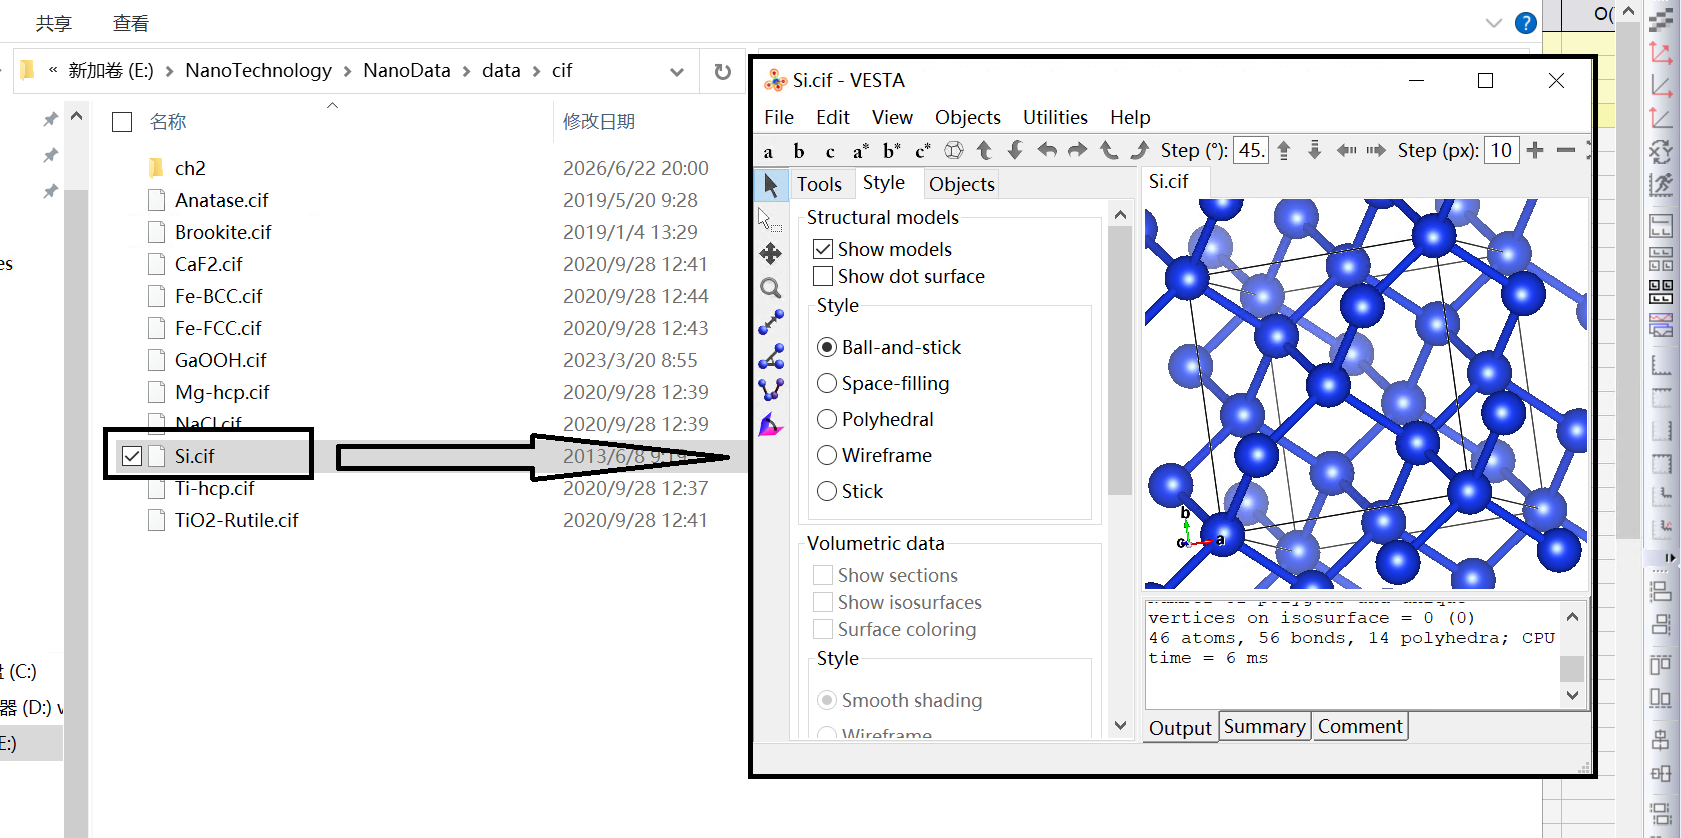
\includegraphics[width=\linewidth]{proc/p01.png}
    \caption{把 Si.cif 拖入 VESTA}
    \label{fig:cif-export-a}
  \end{subfigure}\hfill
  \begin{subfigure}[t]{0.34\linewidth}
    \centering
    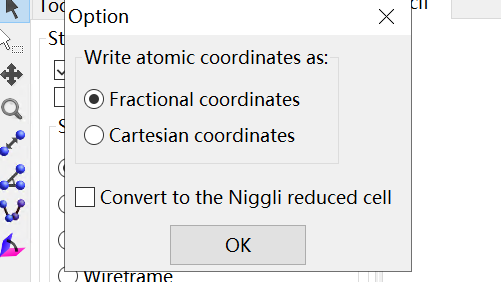
\includegraphics[width=\linewidth]{proc/p02.png}
    \caption{选择分数坐标}
    \label{fig:cif-export-b}
  \end{subfigure}

  \vspace{0.3em}
  \begin{subfigure}[t]{0.26\linewidth}
    \centering
    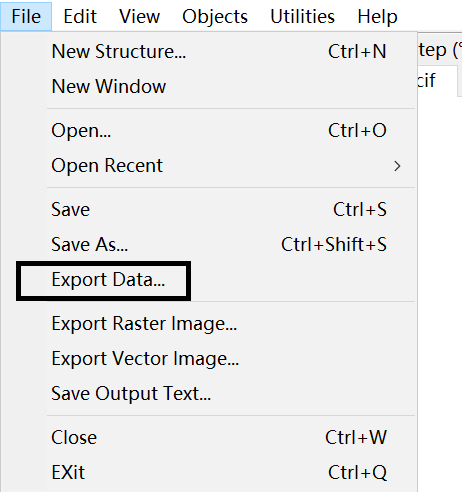
\includegraphics[width=\linewidth]{proc/p03.png}
    \caption{File $\rightarrow$ Export Data}
    \label{fig:cif-export-c}
  \end{subfigure}\hfill
  \begin{subfigure}[t]{0.38\linewidth}
    \centering
    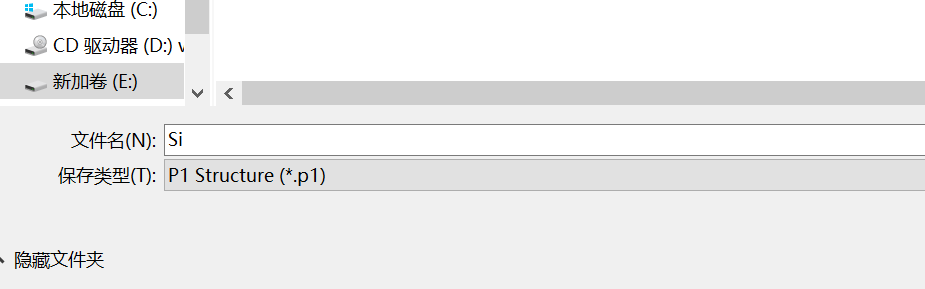
\includegraphics[width=\linewidth]{proc/p04.png}
    \caption{导出为 P1 结构}
    \label{fig:cif-export-d}
  \end{subfigure}

  \vspace{0.3em}
  \begin{subfigure}[t]{0.86\linewidth}
    \centering
    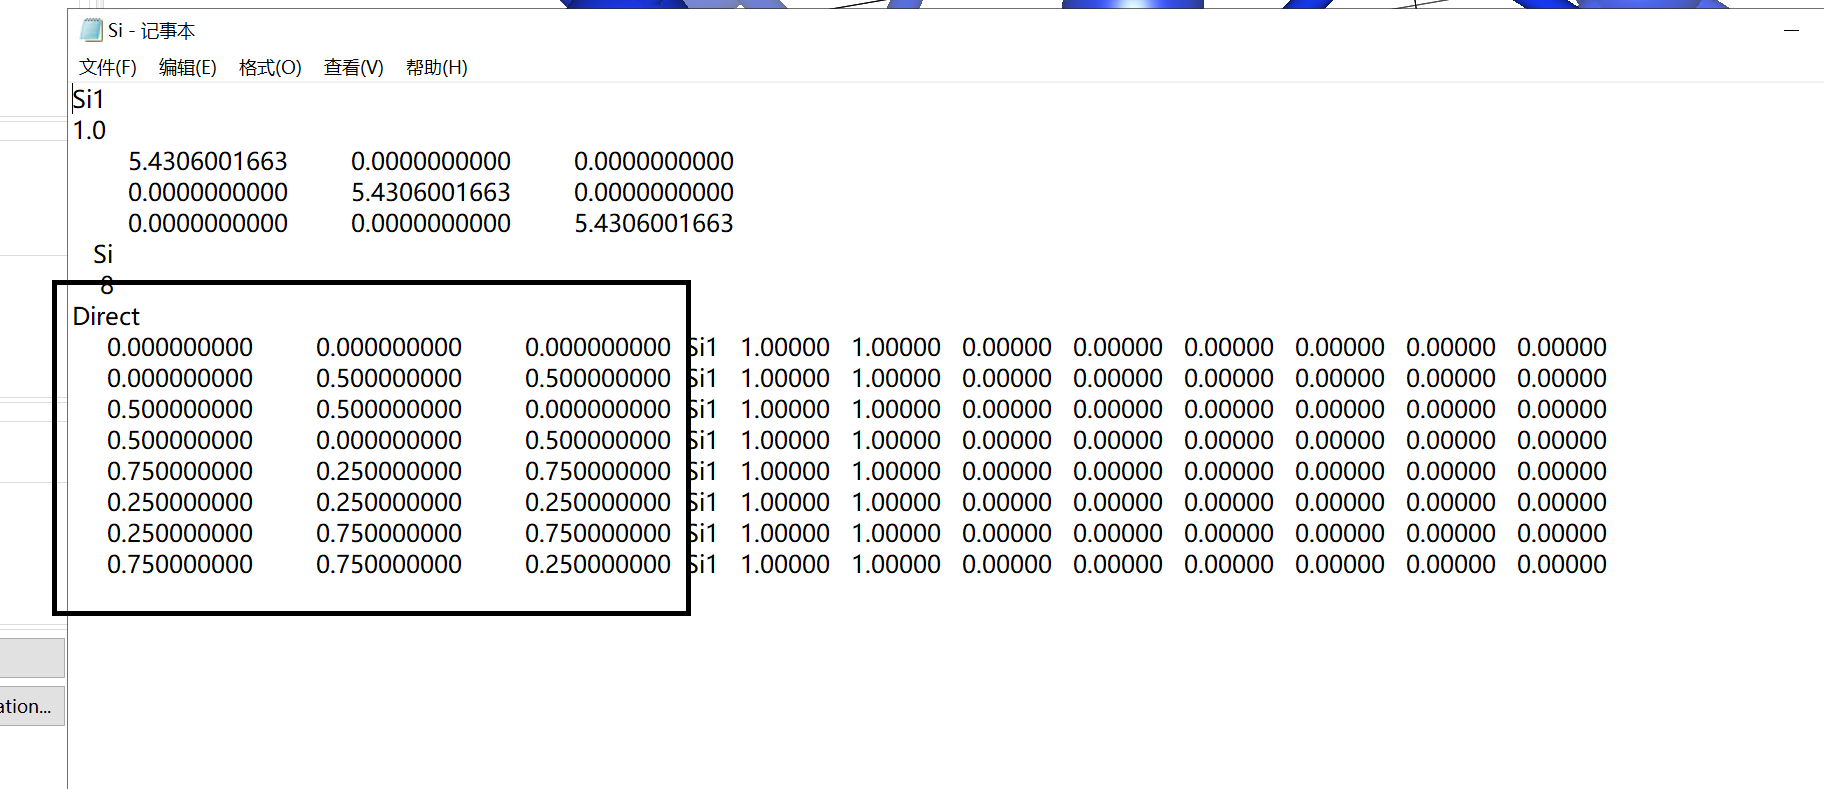
\includegraphics[width=\linewidth]{proc/p05.png}
    \caption{用记事本读取 \texttt{Direct} 坐标块}
    \label{fig:cif-export-e}
  \end{subfigure}
  \caption{从 Si.cif 提取 8 个原子分数坐标：(a) VESTA 显示金刚石结构；(b) 设置为分数坐标；(c)(d) 导出 P1 文件；(e) 记事本中的晶胞参数与 \texttt{Direct} 坐标块。}
  \label{fig:cif-export}
\end{figure}

\subsection{结构因子与消光系数}
\label{sec:f14}

运动学近似下，晶面 $(hkl)$ 的衍射强度正比于结构因子模的平方：
\begin{equation}
I(hkl)\propto|F(hkl)|^2,\qquad
F(hkl)=\sum_{j=1}^{N}g_jt_j(s)f_j(s)\exp\left[2\pi i(hx_j+ky_j+lz_j)\right].
\label{eq:extinction-F}
\end{equation}
当 $|F(hkl)|^2=0$ 时，该晶面不产生衍射，称为消光。本文按课程习惯，把由结构因子得到的相对强度因子 $|F(hkl)|^2$ 称为该晶面的“消光系数”；严格地说，它是运动学近似下的结构因子平方，而不是动力学理论中的消光系数。

图 \ref{fig:structure-factor}(a) 给出了结构因子公式，图 \ref{fig:structure-factor}(b) 给出了 $f=14$ 和 8 个原子的分数坐标，图 \ref{fig:structure-factor}(c)(d) 给出了相位差、实部、虚部和强度的计算。图 \ref{fig:structure-factor}(b)(c)(d) 的表格表头为 $f,x,y,z,h,k,l,\text{phase},\cos,\sin,I$，对应 A--K 列；它只用于消光系数计算，不用于画衍射图。

把表 \ref{tab:si-atoms} 的 8 行坐标放在一起，令
\begin{lstlisting}
phase = 360*(E*B + F*C + G*D)
real  = A*COS(H)
imag  = A*SIN(H)
I     = (TOTAL(I))^2 + (TOTAL(J))^2
\end{lstlisting}
其中 A 为 $f=14$，B、C、D 为原子的 $x,y,z$，E、F、G 为 $h,k,l$，H 为相位。每个衍射点需要 8 行原子坐标；\texttt{TOTAL} 对这 8 行求和，得到 $\sum f\cos\phi$ 和 $\sum f\sin\phi$，再平方相加即得 $|F|^2$。若一次计算多个衍射点，应把每个点的 8 行作为一个块，用 \texttt{SUM} 指定块范围，或增加“斑点编号”列后用 \texttt{TOTALIF} 按编号分组，避免把不同斑点的原子混在一起。

\begin{figure}[H]
  \centering
  \begin{subfigure}[t]{0.96\linewidth}
    \centering
    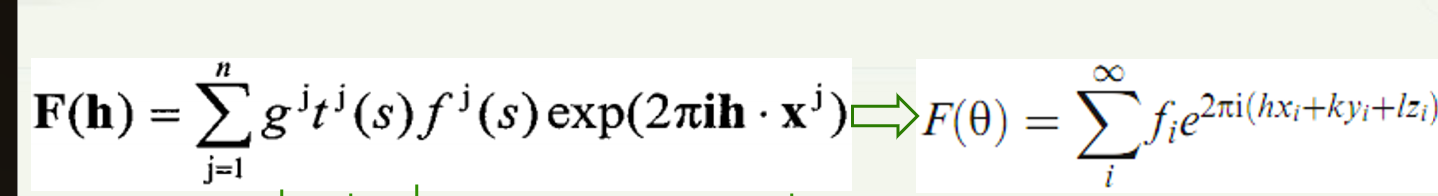
\includegraphics[width=\linewidth]{proc/p16.png}
    \caption{结构因子公式}
    \label{fig:structure-factor-a}
  \end{subfigure}

  \vspace{0.25em}
  \begin{subfigure}[t]{0.62\linewidth}
    \centering
    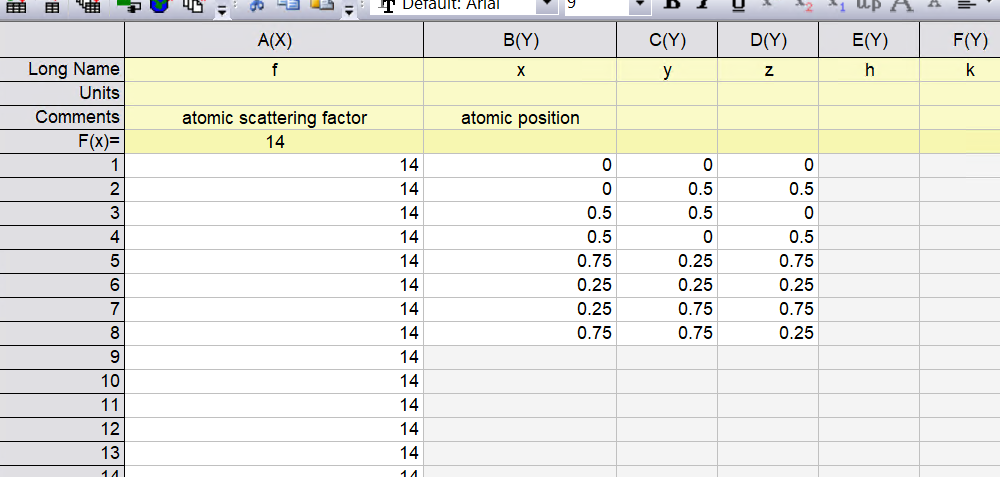
\includegraphics[width=\linewidth]{proc/p17.png}
    \caption{$f=14$（Si 的原子序数）与 8 个原子坐标}
    \label{fig:structure-factor-b}
  \end{subfigure}\hfill
  \begin{subfigure}[t]{0.32\linewidth}
    \centering
    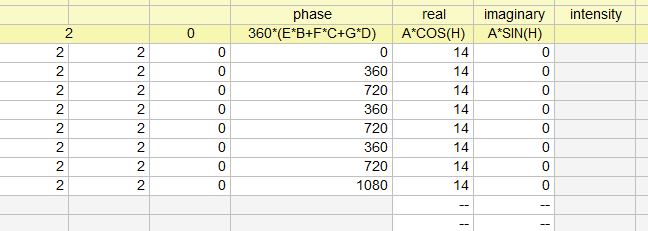
\includegraphics[width=\linewidth]{proc/p18.png}
    \caption{相位差公式}
    \label{fig:structure-factor-c}
  \end{subfigure}

  \vspace{0.25em}
  \begin{subfigure}[t]{0.36\linewidth}
    \centering
    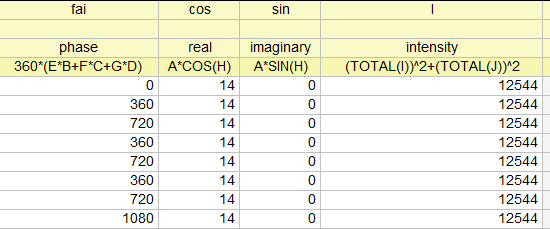
\includegraphics[width=\linewidth]{proc/p19.png}
    \caption{强度公式与结果}
    \label{fig:structure-factor-d}
  \end{subfigure}
  \caption{消光系数（结构因子）的计算：(a) $F(h)=\sum g^jt^j(s)f^j(s)\exp(2\pi i\bm{h}\cdot\bm{x}^j)$；(b) $f=14$ 和 8 个原子的分数坐标，表头为 $f,x,y,z,h,k,l,\text{phase},\cos,\sin,I$；(c) 相位差 $360^\circ(hx+ky+lz)$ 及实部、虚部；(d) 强度 $(\sum\mathrm{real})^2+(\sum\mathrm{imag})^2$。}
  \label{fig:structure-factor}
\end{figure}

图 \ref{fig:structure-factor}(b) 中的 $f=14$ 不是一个随意设定的常数，而是 Si 原子散射因子的前向散射值。原子散射因子 $f$（严格写作 $f(s)$，$s=\sin\theta/\lambda$）表示一个原子在给定方向上的散射振幅与一个自由电子散射振幅之比，量纲为 1；当散射角趋于零时，各电子的散射波完全同相叠加，$f(0)$ 近似等于原子的核外电子数，即原子序数 $Z$。Si 的 $Z=14$，所以模板取 $f=14$，相当于采用 $f(0)$ 这一上限值。真实晶体的 $f(s)$ 随 $\sin\theta/\lambda$ 增大而单调下降，还要乘上温度因子 $t(s)=\exp(-Bs^2)$（第 \ref{sec:cromer-mann} 节 PDF 卡片用的 Cromer--Mann $f(s)$ 就是这种角度依赖的定量表述），因此固定 $f=14$ 属于运动学近似下的最简处理。

这一简化对“是否消光”的判断是充分的：$F(hkl)=0$ 来自晶胞内各原子相位项的完全抵消，与 $f$ 取何值无关，所以用 $f=14$ 算出的零强度点，在真实晶体中同样消光。但它对未消光反射的相对强度只是近似：高角反射的真实 $f(s)$ 已明显小于 14，其强度会被本模板高估，这与表 \ref{tab:pdf-card} 中 $f=14$ 与 $f(s)$ 两列强度的差异是同一原因。

\subsection{110 反射的消光验证}

图 \ref{fig:extinction} 以 110 反射为例验证消光。110 的 $h,k,l$ 为奇偶混合，按第 1 章的规则应有 $F=0$。在表格中输入 $h=k=1$、$l=0$ 后，相位依次为 $0^\circ,180^\circ,360^\circ,\ldots$，8 个原子的实部两两抵消，最终强度约为 $4.7\times10^{-29}$，在数值上就是零。这个结果说明：几何点阵中虽然会出现 110 的位置，但结构因子会使该点消光；实际电子衍射花样中不会看到这个斑点。第 4 章绘制衍射图时，应把这类消光点删除或置零，不能把它们当作真实斑点。

\begin{figure}[H]
  \centering
  \begin{subfigure}[t]{0.20\linewidth}
    \centering
    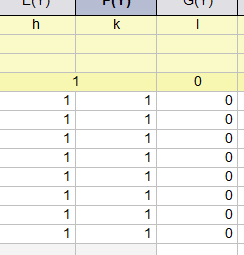
\includegraphics[width=\linewidth]{proc/p20.png}
    \caption{输入 $hkl=110$}
    \label{fig:extinction-a}
  \end{subfigure}\hfill
  \begin{subfigure}[t]{0.46\linewidth}
    \centering
    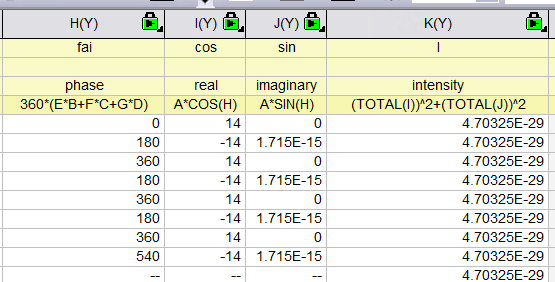
\includegraphics[width=\linewidth]{proc/p21.png}
    \caption{强度全部消光}
    \label{fig:extinction-b}
  \end{subfigure}
  \caption{110 反射的消光验证：(a) 输入 $h=k=1,l=0$；(b) 实部正负抵消，强度约 $4.7\times10^{-29}$。}
  \label{fig:extinction}
\end{figure}

\subsection{单晶硅的消光规律}

把上述计算用于一组典型晶面，可得到表 \ref{tab:extinction-examples}。金刚石结构的消光规律可以归纳为：
\begin{itemize}[leftmargin=2em,itemsep=1pt]
  \item $h,k,l$ 奇偶混合：$|F|^2=0$，消光；
  \item $h,k,l$ 全为偶数且 $h+k+l=4n+2$：$|F|^2=0$，消光；
  \item $h,k,l$ 全为奇数：$|F|^2=32f^2=6272$（$f=14$），允许；
  \item $h,k,l$ 全为偶数且 $h+k+l=4n$：$|F|^2=64f^2=12544$（$f=14$），允许且较强。
\end{itemize}
因此，Si 的允许反射为 111、220、311、400、331、422、511/333、440、531、620 等，而 100、110、200、222、420、600 等消光。第 4 章在每个带轴的几何点阵中会保留所有 $m,n$ 格点，但只有表 \ref{tab:extinction-examples} 中“允许”的格点才是真实衍射斑；实际绘图时应按消光系数表把这些点筛选出来。

\begin{table}[H]
  \centering
  \caption{单晶硅典型晶面的结构因子与消光判断（$f=14$）}
  \label{tab:extinction-examples}
  \small
  \setlength{\tabcolsep}{5pt}
  \renewcommand{\arraystretch}{1.03}
  \begin{tabular}{cccccl}
    \toprule
    $hkl$ & $h+k+l$ & 奇偶性 & $|F|^2$ & 判断 & 说明 \\
    \midrule
    111 & 3 & 全奇 & 6272  & 允许 & $32f^2$ \\
    200 & 2 & 全偶，$4n+2$ & 0 & 消光 & $h+k+l=2$ \\
    220 & 4 & 全偶，$4n$ & 12544 & 允许 & $64f^2$ \\
    222 & 6 & 全偶，$4n+2$ & 0 & 消光 & $h+k+l=6$ \\
    311 & 5 & 全奇 & 6272  & 允许 & $32f^2$ \\
    400 & 4 & 全偶，$4n$ & 12544 & 允许 & $64f^2$ \\
    331 & 7 & 全奇 & 6272  & 允许 & $32f^2$ \\
    420 & 6 & 全偶，$4n+2$ & 0 & 消光 & $h+k+l=6$ \\
    422 & 8 & 全偶，$4n$ & 12544 & 允许 & $64f^2$ \\
    511/333 & 7/9 & 全奇 & 6272 & 允许 & $32f^2$ \\
    440 & 8 & 全偶，$4n$ & 12544 & 允许 & $64f^2$ \\
    531 & 9 & 全奇 & 6272 & 允许 & $32f^2$ \\
    600 & 6 & 全偶，$4n+2$ & 0 & 消光 & $h+k+l=6$ \\
    620 & 8 & 全偶，$4n$ & 12544 & 允许 & $64f^2$ \\
    \bottomrule
  \end{tabular}
\end{table}

% ==================== 4 单晶硅带轴电子衍射模拟 ====================
\section{单晶硅带轴电子衍射模拟}

\subsection{模拟思路}

第 3 章已经得到每个晶面的消光系数和允许/消光判断。本章的任务是把允许的反射排布到二维倒易面上。电子束沿 $[uvw]$ 方向入射时，属于该带轴的晶面满足晶带方程 $hu+kv+lw=0$，这些晶面的倒易点构成过原点的二维倒易面 $(uvw)^*$。在二维倒易面内选取两条不共线的基矢 $\bm{g}_1=(h_1k_1l_1)^*$、$\bm{g}_2=(h_2k_2l_2)^*$，就可以用整数 $m,n$ 把整个倒易面展开，再由式 \eqref{eq:xy} 和式 \eqref{eq:hkl-mn} 得到每个衍射点的二维坐标和晶面指数。最后，用第 3 章的消光系数表筛选允许的反射，再用二维散点图和三维 Waterfall 图显示。

具体流程如下：
\begin{enumerate}[label=（\arabic*）,leftmargin=2.2em,itemsep=1pt]
  \item 对给定带轴 $[uvw]$，选取两条满足 $hu+kv+lw=0$ 的低指数反射作为 $\bm{g}_1,\bm{g}_2$，并用叉积确认 $\bm{g}_1\times\bm{g}_2\parallel[uvw]$；
  \item 用第 2 章的模板计算 $r_1,r_2,\theta$；
  \item 建立衍射图表格，计算 $x,y,h,k,l$，并把强度初值设为 100，得到几何点阵；
  \item 按第 3 章的消光系数表筛选允许的反射，把消光点删除或置零；
  \item 用二维散点图和三维 Waterfall 图显示结果。
\end{enumerate}

\subsection{基矢的确定与 \texorpdfstring{$r_1$、$r_2$、$\theta$}{r1、r2、theta} 的计算}

带轴确定后，基矢的选法不唯一，但必须满足两个条件：两条反射都满足晶带方程，且叉积 $\bm{g}_1\times\bm{g}_2$ 平行于带轴。需要说明的是，基矢只要求是倒易格点且不共线，并不要求基矢本身是强反射；例如 [111] 的 $(\bar{1}01)^*$ 和 $(0\bar{1}1)^*$ 本身是消光点，但它们的整数组合可以生成 220、422 等允许反射。实际哪些点出现，仍由结构因子决定。以 [421] 带轴为例，$(-120)$ 和 $(-104)$ 都满足
\begin{equation}
4h+2k+l=0,
\end{equation}
因为它们分别给出 $4(-1)+2(2)+0=0$ 和 $4(-1)+2(0)+4=0$；二者的叉积为 $(8,4,2)\parallel[421]$。把这两组指数输入第 2 章的模板，即可得到对应的 $r_1$、$r_2$ 和 $\theta$。图 \ref{fig:basis-calc}(a) 给出了在计算器中输入 $(-120)$、$(-104)$ 的界面，图 \ref{fig:basis-calc}(b) 给出了 $r_1,r_2,\theta$ 的结果，图 \ref{fig:basis-calc}(c) 则是把 $r_1,r_2,\theta$ 代入式 \eqref{eq:xy} 后得到的二维点阵示意。这个 [421] 例子只用于说明方法；本作业要求的五个带轴的基矢和计算结果列于表 \ref{tab:zone-params}。

\begin{figure}[H]
  \centering
  \begin{subfigure}[t]{0.62\linewidth}
    \centering
    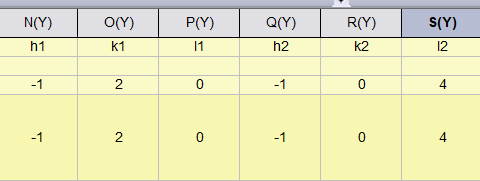
\includegraphics[width=\linewidth]{proc/p06.png}
    \caption{输入 $(-120)$、$(-104)$ 两组晶面}
    \label{fig:basis-calc-a}
  \end{subfigure}\hfill
  \begin{subfigure}[t]{0.14\linewidth}
    \centering
    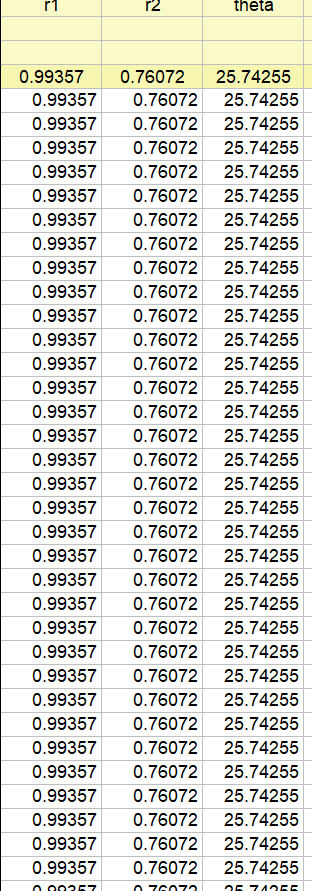
\includegraphics[height=4.6cm]{proc/p07.png}
    \caption{$r_1,r_2,\theta$ 结果}
    \label{fig:basis-calc-b}
  \end{subfigure}

  \vspace{0.3em}
  \begin{subfigure}[t]{0.72\linewidth}
    \centering
    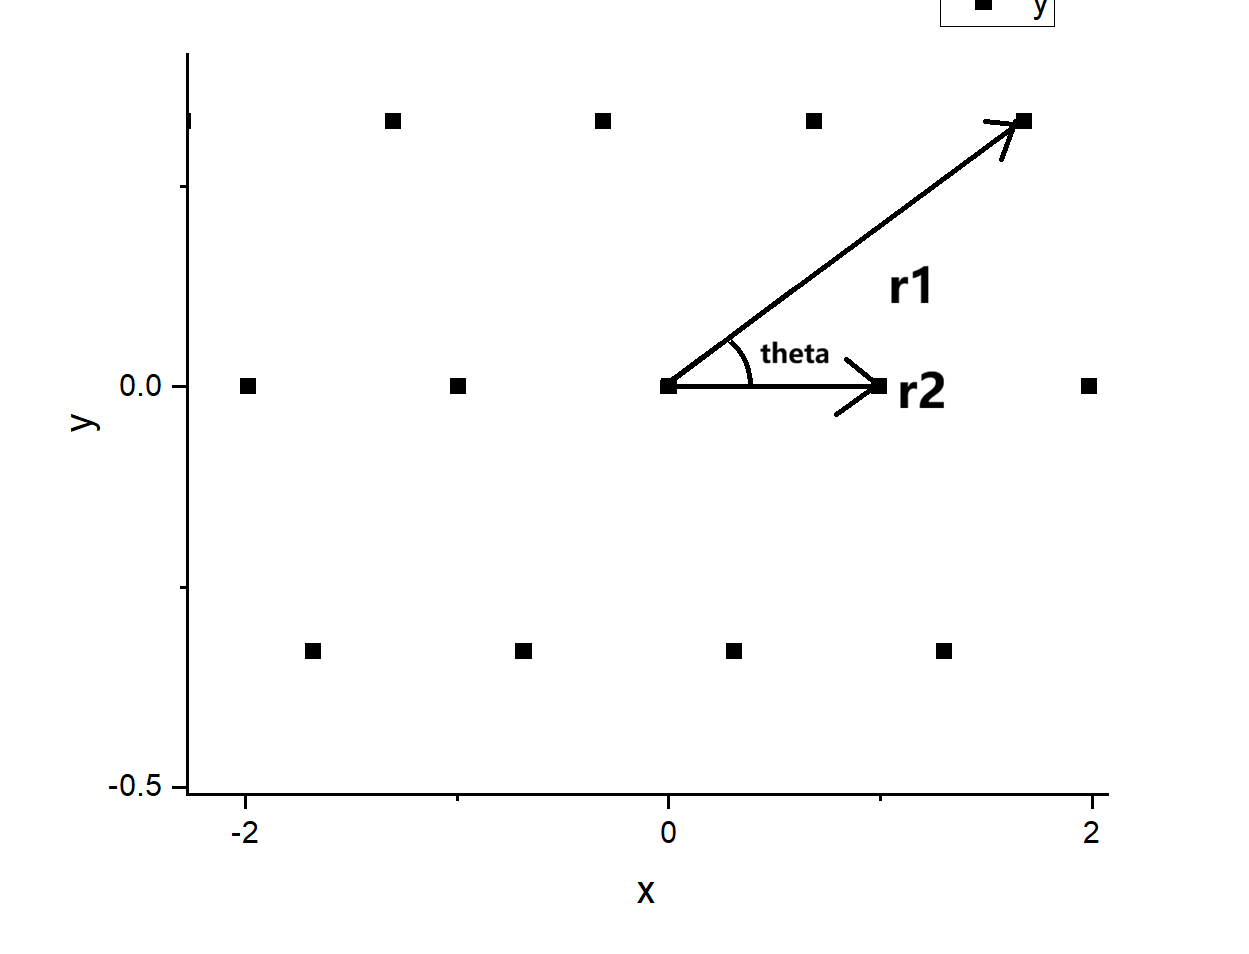
\includegraphics[width=\linewidth]{proc/p08.png}
    \caption{放大后的二维点阵与基矢}
    \label{fig:basis-calc-c}
  \end{subfigure}
  \caption{以 [421] 带轴为例确定基矢：(a) 在计算器中输入 $(-120)$、$(-104)$；(b) 得到 $r_1,r_2,\theta$；(c) 由式 \eqref{eq:xy} 得到的二维点阵。图 (b) 的数值为软件当前表格的显示值，仅用于说明 T--V 三列的位置；五个带轴的实际结果以表 \ref{tab:zone-params} 为准。}
  \label{fig:basis-calc}
\end{figure}

\begin{table}[H]
  \centering
  \caption{五个带轴的基矢、倒易矢量长度、夹角与二维点阵类型（单晶硅，$a=5.43$~\AA）}
  \label{tab:zone-params}
  \small
  \setlength{\tabcolsep}{4pt}
  \renewcommand{\arraystretch}{1.08}
  \begin{tabular}{ccccccc}
    \toprule
    带轴 $[uvw]$ & $\bm{g}_1=(h_1k_1l_1)^*$ & $\bm{g}_2=(h_2k_2l_2)^*$ & $r_1$/\AA$^{-1}$ & $r_2$/\AA$^{-1}$ & $\theta$/$^\circ$ & 二维点阵 \\
    \midrule
    {}[001] & $(100)^*$  & $(010)^*$  & 0.18416 & 0.18416 & 90.0000  & 正方 \\
    {}[111] & $(\bar{1}01)^*$ & $(0\bar{1}1)^*$ & 0.26044 & 0.26044 & 120.0000 & 三角/六方 \\
    {}[332] & $(2\bar{2}0)^*$ & $(04\bar{6})^*$ & 0.52089 & 1.32801 & 113.0935 & 斜方 \\
    {}[334] & $(2\bar{2}0)^*$ & $(08\bar{6})^*$ & 0.52089 & 1.84162 & 124.4499 & 斜方 \\
    {}[345] & $(2\bar{4}2)^*$ & $(\bar{6}22)^*$ & 0.90221 & 1.22159 & 119.4962 & 斜方 \\
    \bottomrule
  \end{tabular}
\end{table}

表 \ref{tab:zone-params} 中的 $r_1,r_2$ 都可由立方晶系的解析式 $r=\sqrt{h^2+k^2+l^2}/a$ 校验。例如 [332] 的 $\bm{g}_2=(04\bar{6})$，$r_2=\sqrt{0^2+4^2+6^2}/5.43=\sqrt{52}/5.43=1.32801$~\AA$^{-1}$；[345] 的 $\bm{g}_1=(2\bar{4}2)$，$r_1=\sqrt{2^2+4^2+2^2}/5.43=\sqrt{24}/5.43=0.90221$~\AA$^{-1}$。夹角也可用式 \eqref{eq:cubic-check} 抽查。若模板结果与解析式不符，应优先检查角度单位和公式中的交叉项。


\subsection{衍射图表格的建立}

新建一个工作表，按 \texttt{r1, r2, theta, m, n, x, y, I, h, k, l} 的顺序建立列，如图 \ref{fig:diff-table}(a)(b) 所示。$m$、$n$ 是二维点阵的整数坐标，图 \ref{fig:diff-table}(c)(d) 中把它们的范围设为 $-5\sim5$，共 $11\times11=121$ 个点。这个范围决定了视场大小：若点阵没有铺满绘图区，可把范围扩大到 $-8\sim8$ 或更大；若只想看中心区域，则可缩小范围。

$x,y$ 两列按式 \eqref{eq:xy} 输入：
\begin{lstlisting}
x = D*A + E*B*COS(C)
y = E*B*SIN(C)
\end{lstlisting}
其中 A、B、C 分别为 $r_1,r_2,\theta$，D、E 分别为 $m,n$。注意 \texttt{COS}、\texttt{SIN} 的自变量是角度，因此角度单位仍须为 Degree。$h,k,l$ 三列按式 \eqref{eq:hkl-mn} 计算。若按附录 A 的推荐列布局，把 $h_1,k_1,l_1$ 放在 L、M、N 列，把 $h_2,k_2,l_2$ 放在 O、P、Q 列，则
\begin{lstlisting}
h = D*L + E*O
k = D*M + E*P
l = D*N + E*Q
\end{lstlisting}
图 \ref{fig:diff-table}(b) 的列名与图 \ref{fig:diff-coords}(c) 的 h、k、l 列就是按这一思路建立的。

\begin{figure}[H]
  \centering
  \begin{subfigure}[t]{0.96\linewidth}
    \centering
    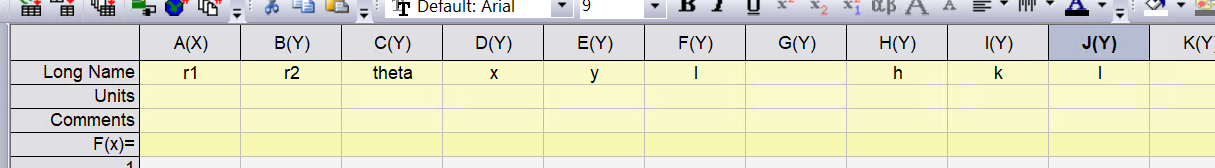
\includegraphics[width=\linewidth]{proc/p09.png}
    \caption{新建衍射图工作表}
    \label{fig:diff-table-a}
  \end{subfigure}

  \vspace{0.25em}
  \begin{subfigure}[t]{0.96\linewidth}
    \centering
    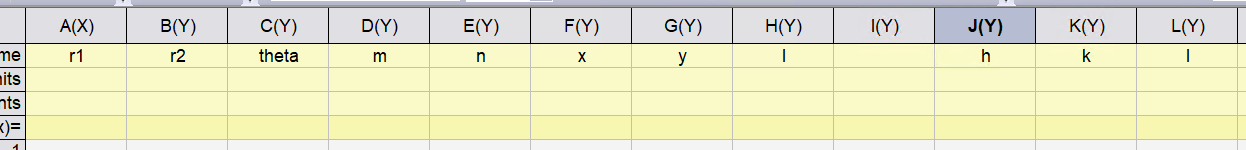
\includegraphics[width=\linewidth]{proc/p10.png}
    \caption{设置列名}
    \label{fig:diff-table-b}
  \end{subfigure}

  \vspace{0.25em}
  \begin{subfigure}[t]{0.32\linewidth}
    \centering
    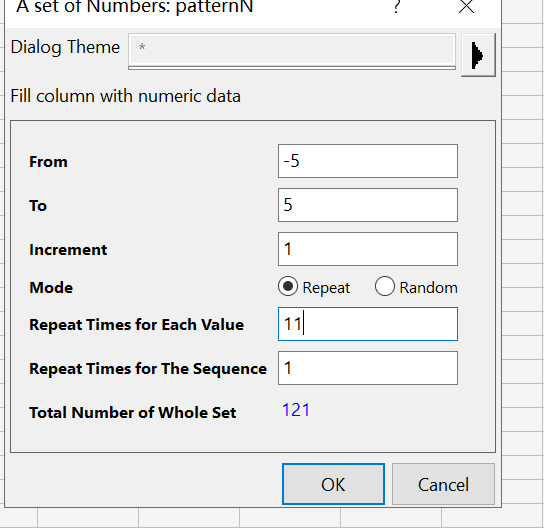
\includegraphics[width=\linewidth]{proc/p11.png}
    \caption{设置 $m$ 的范围}
    \label{fig:diff-table-c}
  \end{subfigure}\hfill
  \begin{subfigure}[t]{0.32\linewidth}
    \centering
    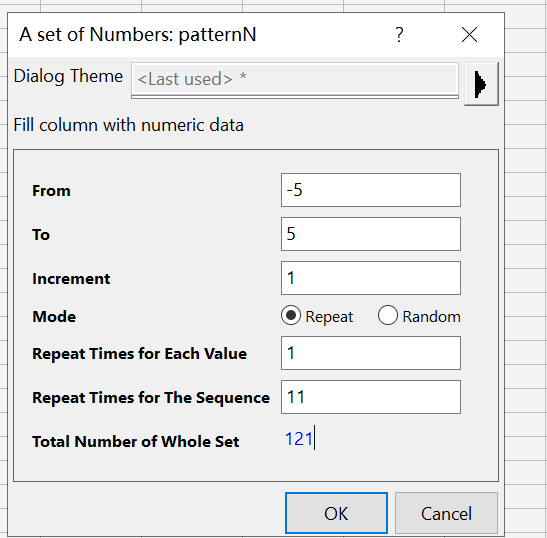
\includegraphics[width=\linewidth]{proc/p12.png}
    \caption{设置 $n$ 的范围}
    \label{fig:diff-table-d}
  \end{subfigure}
  \caption{衍射图表格的建立：(a) 新建工作表；(b) 设置 \texttt{r1, r2, theta, m, n, x, y, I, h, k, l} 等列；(c)(d) 用 \texttt{-5} 到 \texttt{5}、步长 1 填充 $m,n$。}
  \label{fig:diff-table}
\end{figure}

\begin{figure}[H]
  \centering
  \begin{subfigure}[t]{0.20\linewidth}
    \centering
    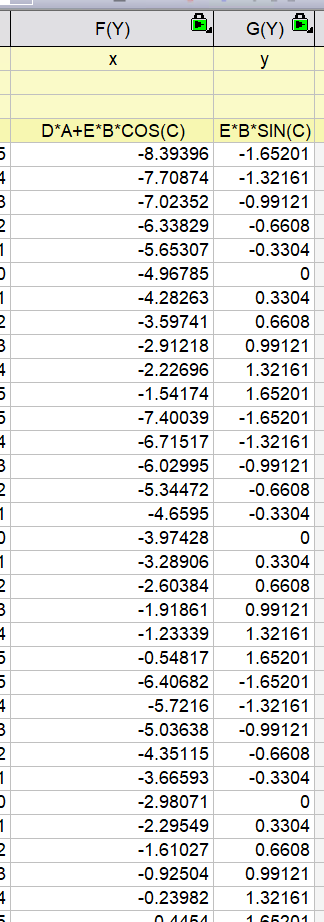
\includegraphics[height=5.2cm]{proc/p13.png}
    \caption{$x,y$ 公式}
    \label{fig:diff-coords-a}
  \end{subfigure}\hfill
  \begin{subfigure}[t]{0.24\linewidth}
    \centering
    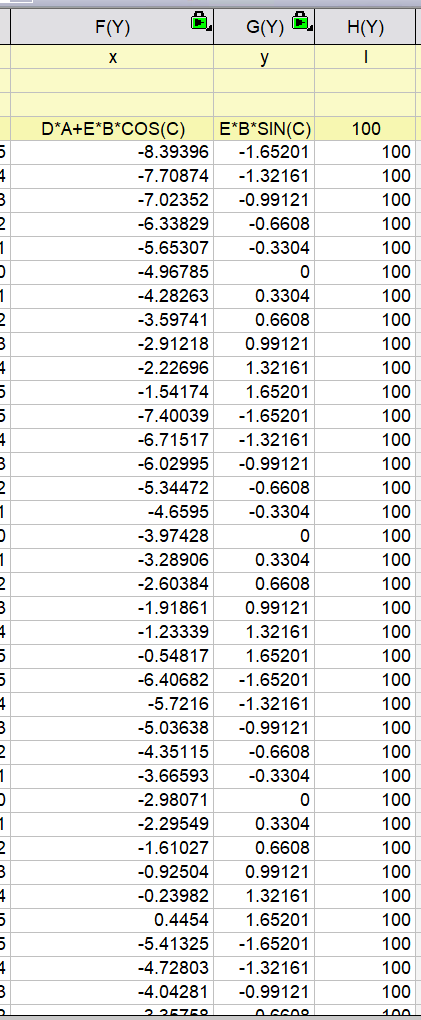
\includegraphics[height=5.2cm]{proc/p14.png}
    \caption{强度初值设为 100}
    \label{fig:diff-coords-b}
  \end{subfigure}\hfill
  \begin{subfigure}[t]{0.20\linewidth}
    \centering
    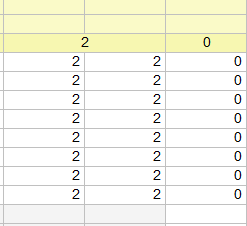
\includegraphics[width=\linewidth]{proc/p15.png}
    \caption{当前 $h,k,l$}
    \label{fig:diff-coords-c}
  \end{subfigure}
  \caption{坐标与指数的计算：(a) 按式 \eqref{eq:xy} 输入 $x,y$；(b) 几何模拟时把 $I$ 统一设为 100；(c) 当前衍射点的 $h,k,l$。}
  \label{fig:diff-coords}
\end{figure}


\subsection{绘图与五个带轴的结果}

\begin{figure}[H]
  \centering
  \begin{subfigure}[t]{0.34\linewidth}
    \centering
    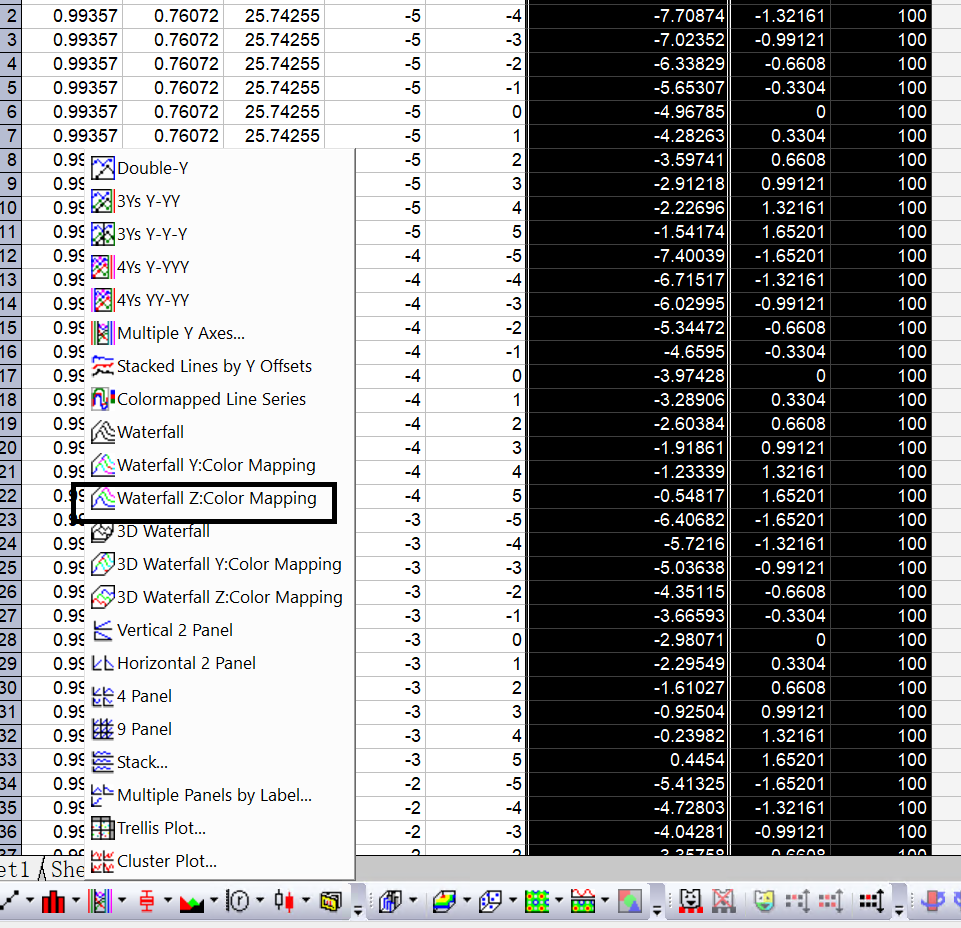
\includegraphics[width=\linewidth]{proc/p22.png}
    \caption{选择 3D Waterfall（WaterfallZ）}
    \label{fig:plot-setup-a}
  \end{subfigure}\hfill
  \begin{subfigure}[t]{0.46\linewidth}
    \centering
    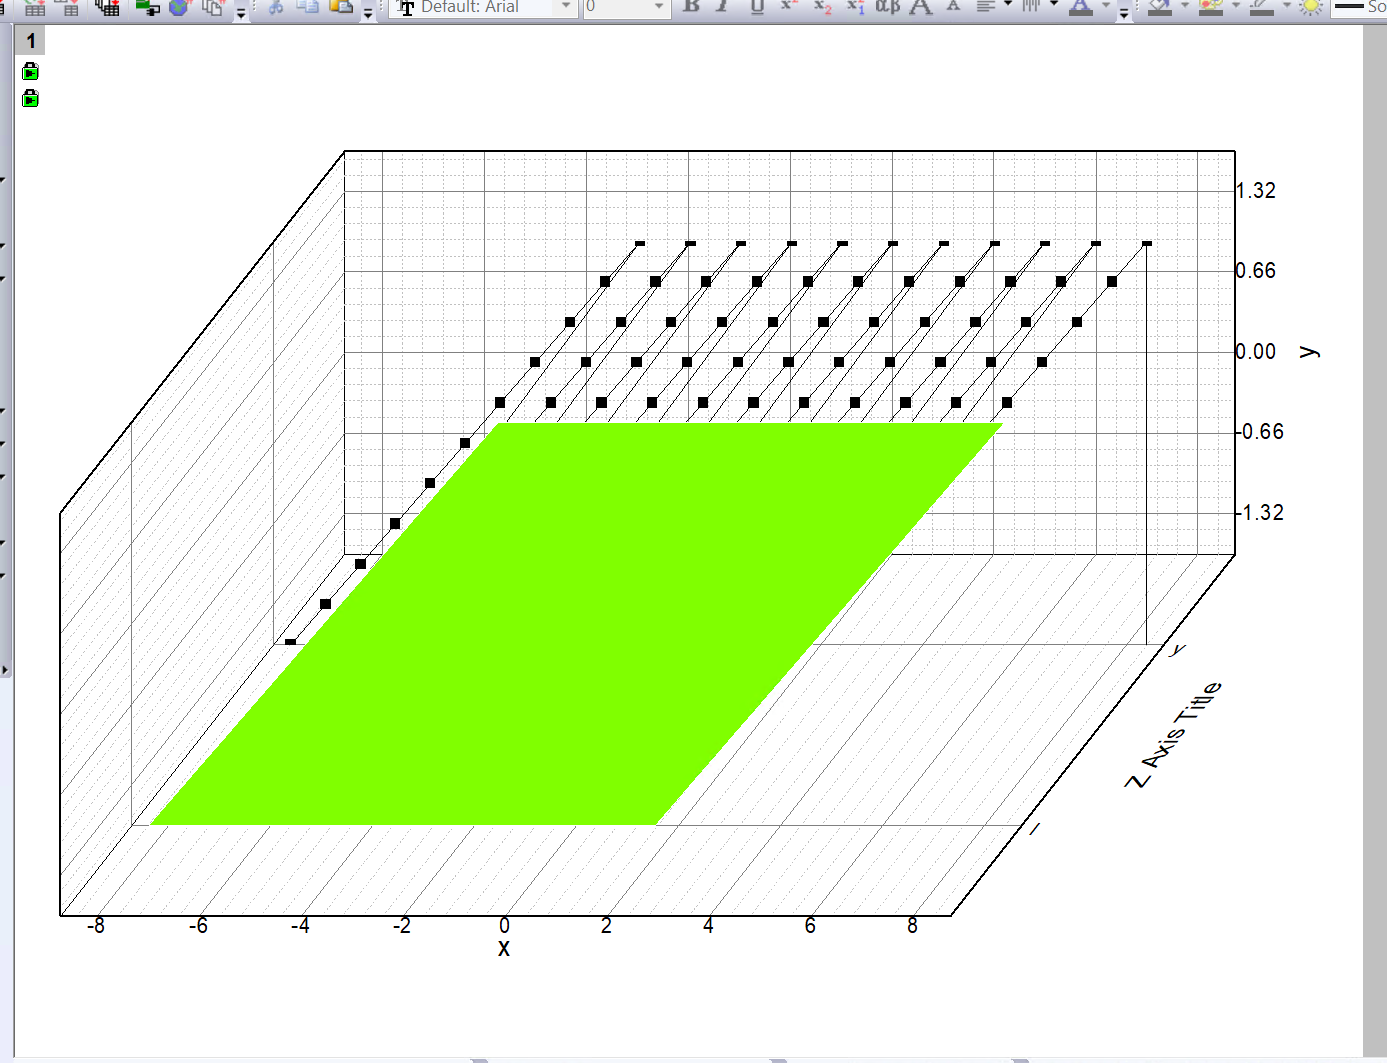
\includegraphics[width=\linewidth]{proc/p23.png}
    \caption{三维 Waterfall 示例}
    \label{fig:plot-setup-b}
  \end{subfigure}

  \vspace{0.3em}
  \begin{subfigure}[t]{0.44\linewidth}
    \centering
    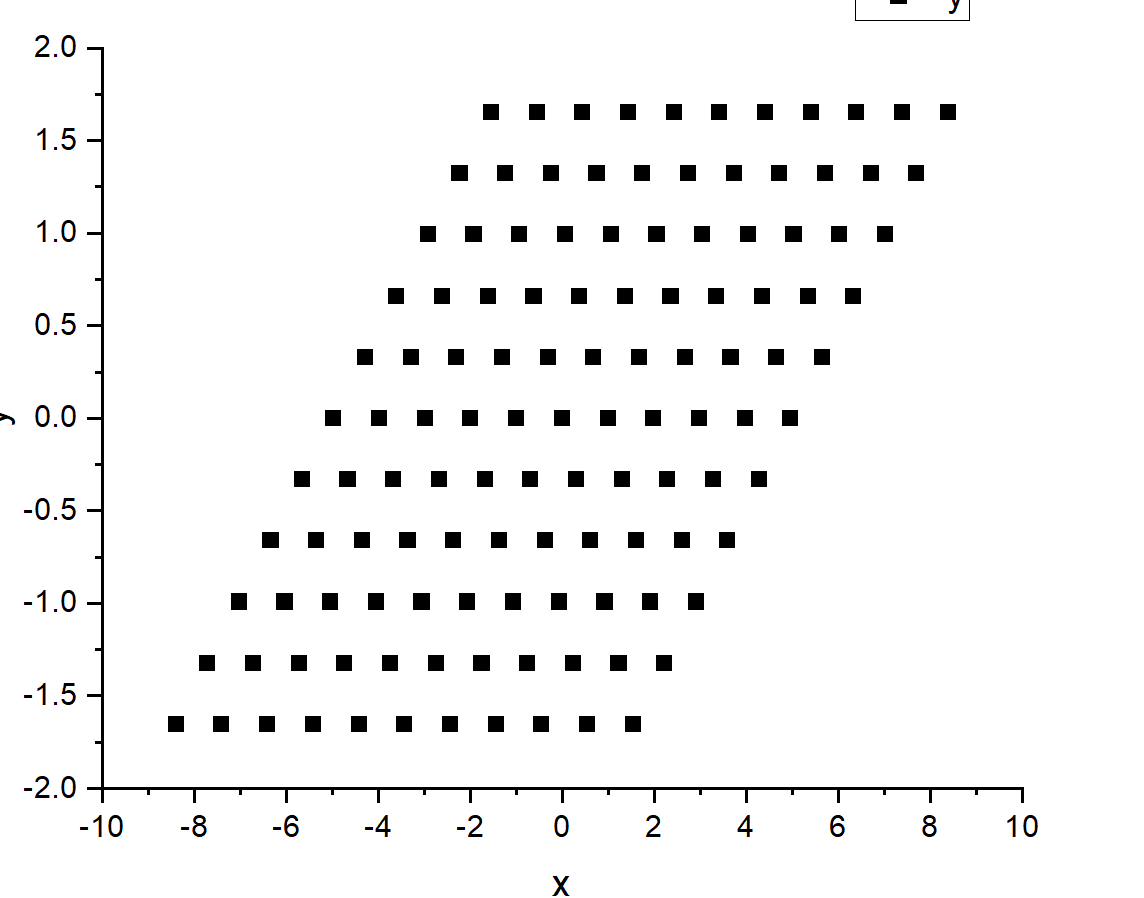
\includegraphics[width=\linewidth]{proc/p24.png}
    \caption{二维散点示例}
    \label{fig:plot-setup-c}
  \end{subfigure}
  \caption{Origin 绘图设置与示例：(a) 选择 3D Waterfall（WaterfallZ）；(b) 三维 Waterfall 图（绿色平面为默认填充对象）；(c) 二维散点图（示例为 [421] 带轴）。}
  \label{fig:plot-setup}
\end{figure}

有了 $x,y,I$ 三列，就可以绘图。二维图选择 \texttt{Plot $\rightarrow$ Scatter}，以 $x$ 为横轴、$y$ 为纵轴；三维图选择 \texttt{Plot $\rightarrow$ 3D Waterfall}，以 $x,y$ 为平面坐标、$I$ 为高度。图 \ref{fig:plot-setup}(a) 是 Waterfall 的设置界面，图 \ref{fig:plot-setup}(b) 是三维示例，图 \ref{fig:plot-setup}(c) 是二维散点示例。三维图中出现的绿色平面是 Origin 默认生成的填充对象（或当前选中的图层），它会遮挡部分数据；正式绘图时应在 \texttt{Plot Details} 中删除该对象，或把填充透明度设为 0。本文保留原始截图，以说明这一常见问题。

以下五组图分别给出 [001]、[111]、[332]、[334]、[345] 五个带轴的计算界面、坐标复制、二维散点图和三维 Waterfall 图。每组图中的 (a) 是 Origin 计算模板中输入的基矢与 $r_1,r_2,\theta$，(b) 是把 $r_1,r_2,\theta$ 复制到衍射图表格后的列数据，(c)(d) 是最终的点阵图。由于几何模拟把 $I$ 统一设为 100，(c)(d) 中所有点的高度相同；实际强度需按第 3 章的消光系数表筛选，消光点应删除或置零。

\subsubsection{[001] 带轴}

[001] 带轴的基矢为 $\bm{g}_1=(100)^*$、$\bm{g}_2=(010)^*$，$r_1=r_2=0.18416$~\AA$^{-1}$，$\theta=90^\circ$。二维点阵是正方形，具有 4 次对称；$m,n$ 取 $-5\sim5$ 时，视场内约有 $11\times11$ 个点。由于金刚石结构的消光，实际允许的反射是 220、400、440、620 等，100、110、200 等不出现。图 \ref{fig:zone001}(c)(d) 中所有点高度相同，是因为几何模拟把 $I$ 统一设为 100；若把 $I$ 换成结构因子列，100、110、200 等点会消失，只剩 220、400 等强点。

\begin{figure}[H]
  \centering
  \begin{subfigure}[t]{0.64\linewidth}
    \centering
    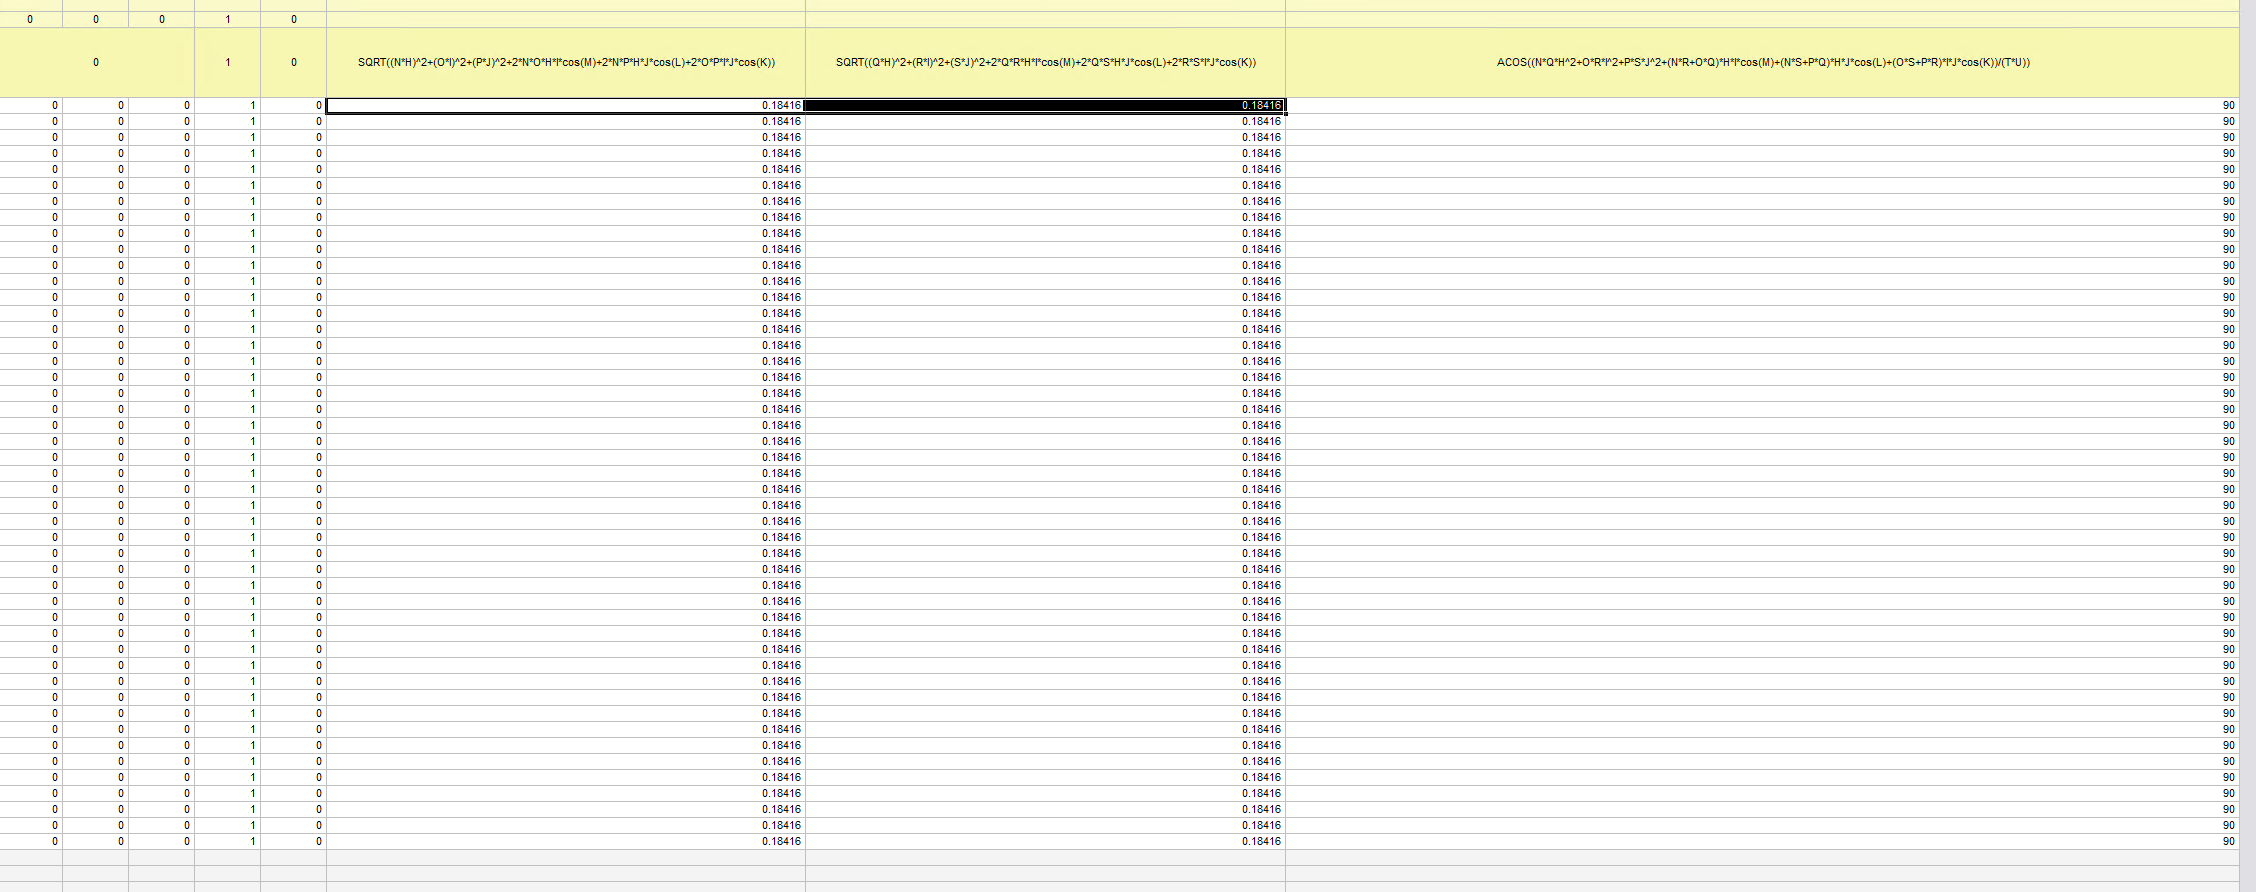
\includegraphics[width=\linewidth]{zone001/zone001_a.png}
    \caption{基矢与 $r_1,r_2,\theta$}
    \label{fig:zone001-a}
  \end{subfigure}\hfill
  \begin{subfigure}[t]{0.14\linewidth}
    \centering
    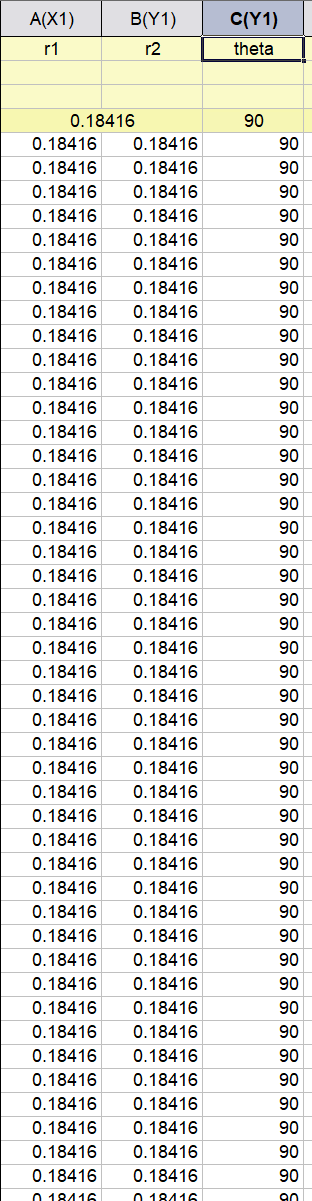
\includegraphics[height=4.3cm]{zone001/zone001_b.png}
    \caption{坐标复制}
    \label{fig:zone001-b}
  \end{subfigure}

  \vspace{0.3em}
  \begin{subfigure}[t]{0.48\linewidth}
    \centering
    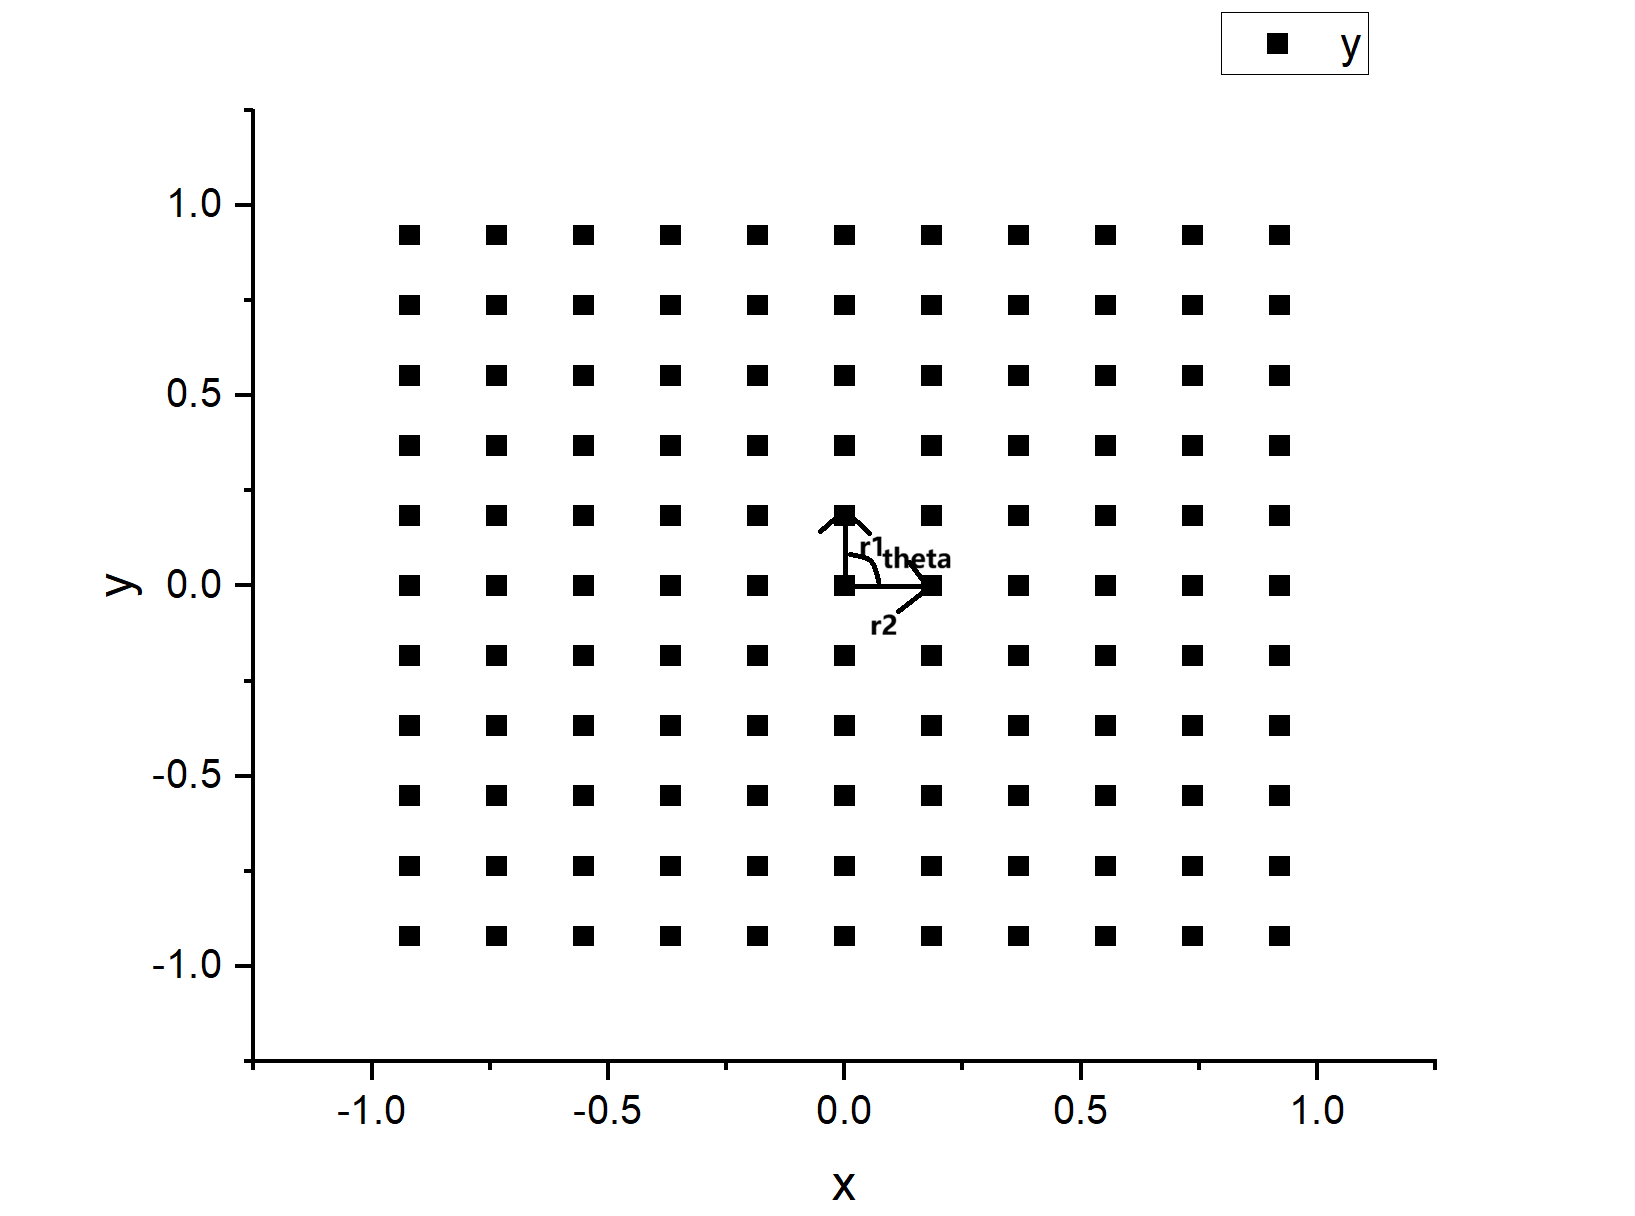
\includegraphics[width=\linewidth]{zone001/zone001_c.png}
    \caption{二维散点图}
    \label{fig:zone001-c}
  \end{subfigure}\hfill
  \begin{subfigure}[t]{0.48\linewidth}
    \centering
    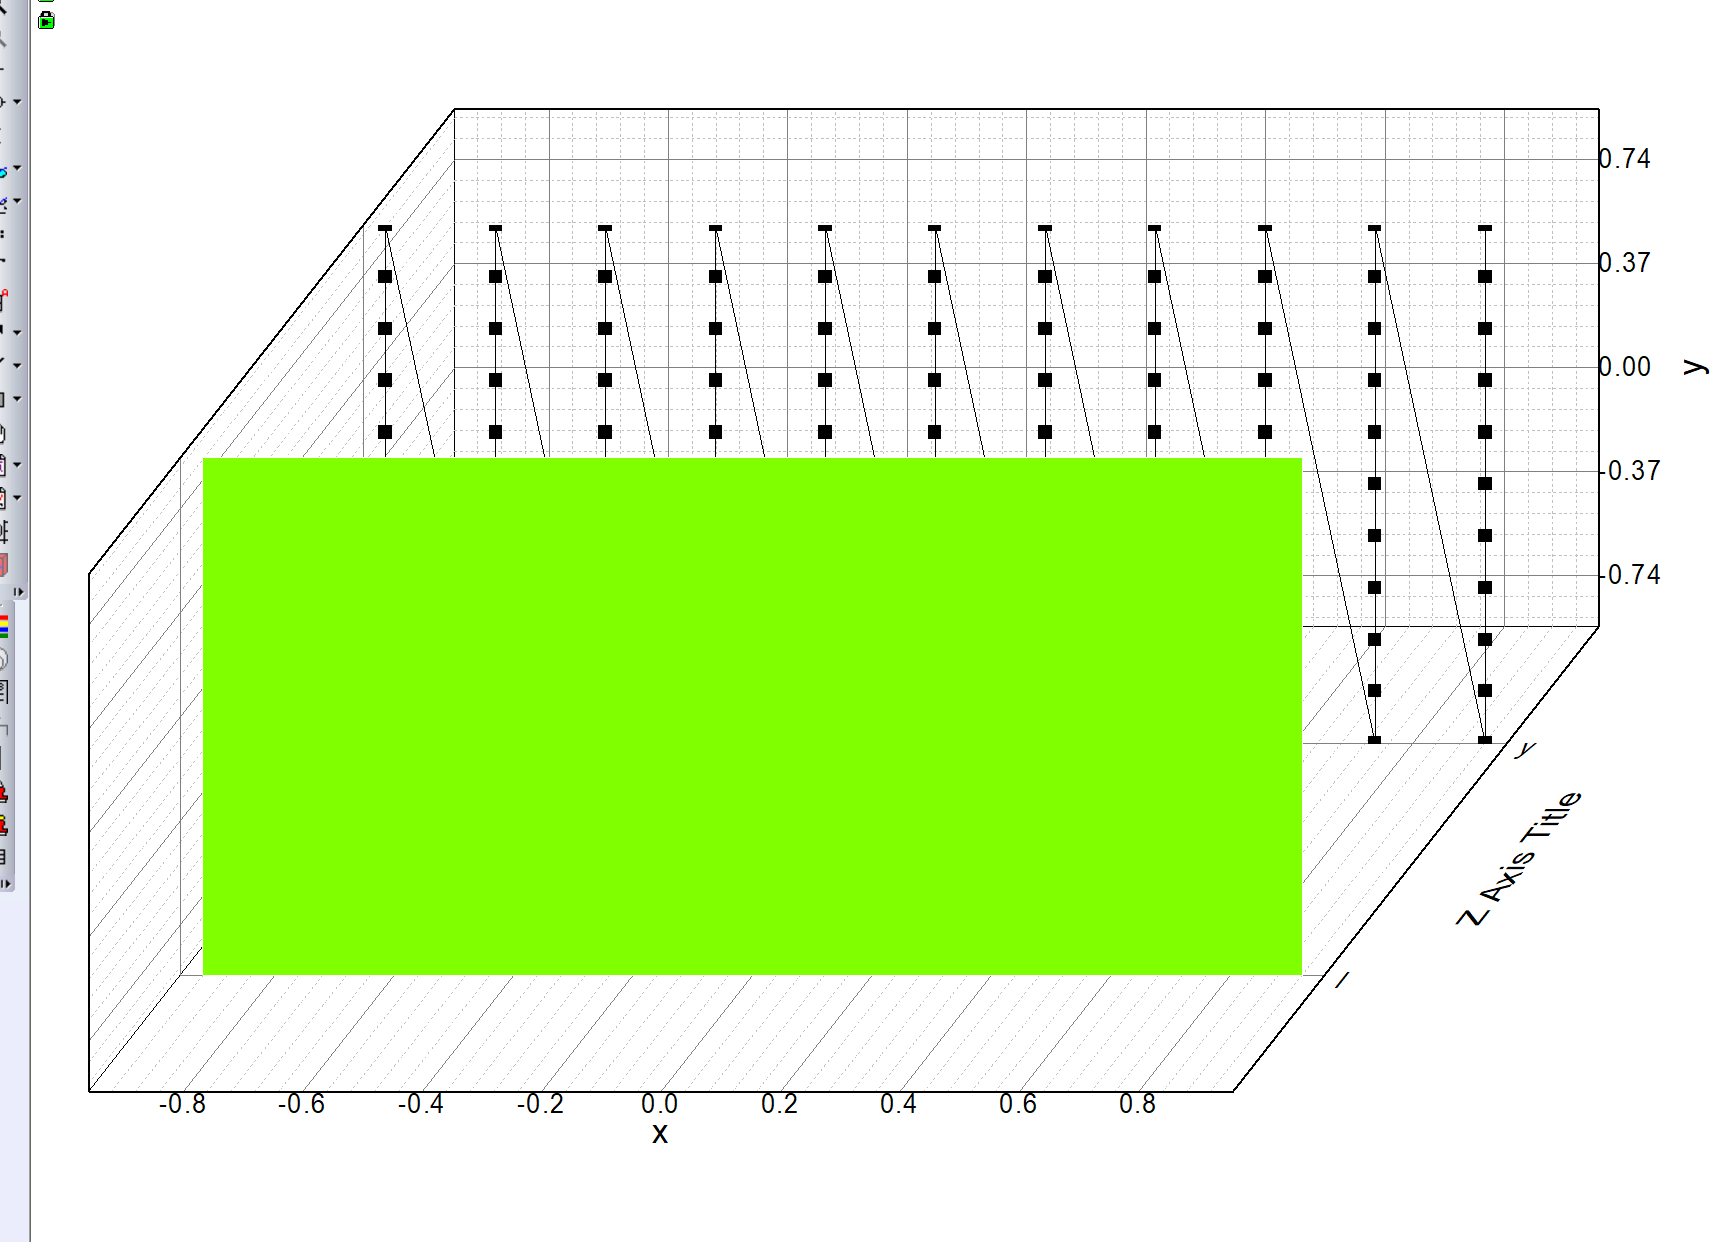
\includegraphics[width=\linewidth]{zone001/zone001_d.png}
    \caption{三维 Waterfall 图}
    \label{fig:zone001-d}
  \end{subfigure}
  \caption{[001] 带轴电子衍射模拟：(a) 基矢 $(100)^*$、$(010)^*$ 与 $r_1=r_2=0.18416$~\AA$^{-1}$、$\theta=90^\circ$；(b) 把 $r_1,r_2,\theta$ 复制到衍射图表格；(c) 正方形二维点阵；(d) 三维 Waterfall 图（绿色平面为默认填充对象）。}
  \label{fig:zone001}
\end{figure}

\subsubsection{[111] 带轴}

[111] 带轴的基矢为 $\bm{g}_1=(\bar{1}01)^*$、$\bm{g}_2=(0\bar{1}1)^*$，$r_1=r_2=0.26044$~\AA$^{-1}$，$\theta=120^\circ$。二维点阵是三角/六方点阵，基矢夹角 $120^\circ$；点阵本身具有 6 次对称，实际衍射强度受结构因子调制，可能出现 3 次对称。允许的反射为 220、422、440 等；111 本身不满足 $hu+kv+lw=0$，属于高阶劳厄带，不在零阶劳厄区内。与 [001] 相比，[111] 的点阵更疏，斑点呈六方排列。

\begin{figure}[H]
  \centering
  \begin{subfigure}[t]{0.64\linewidth}
    \centering
    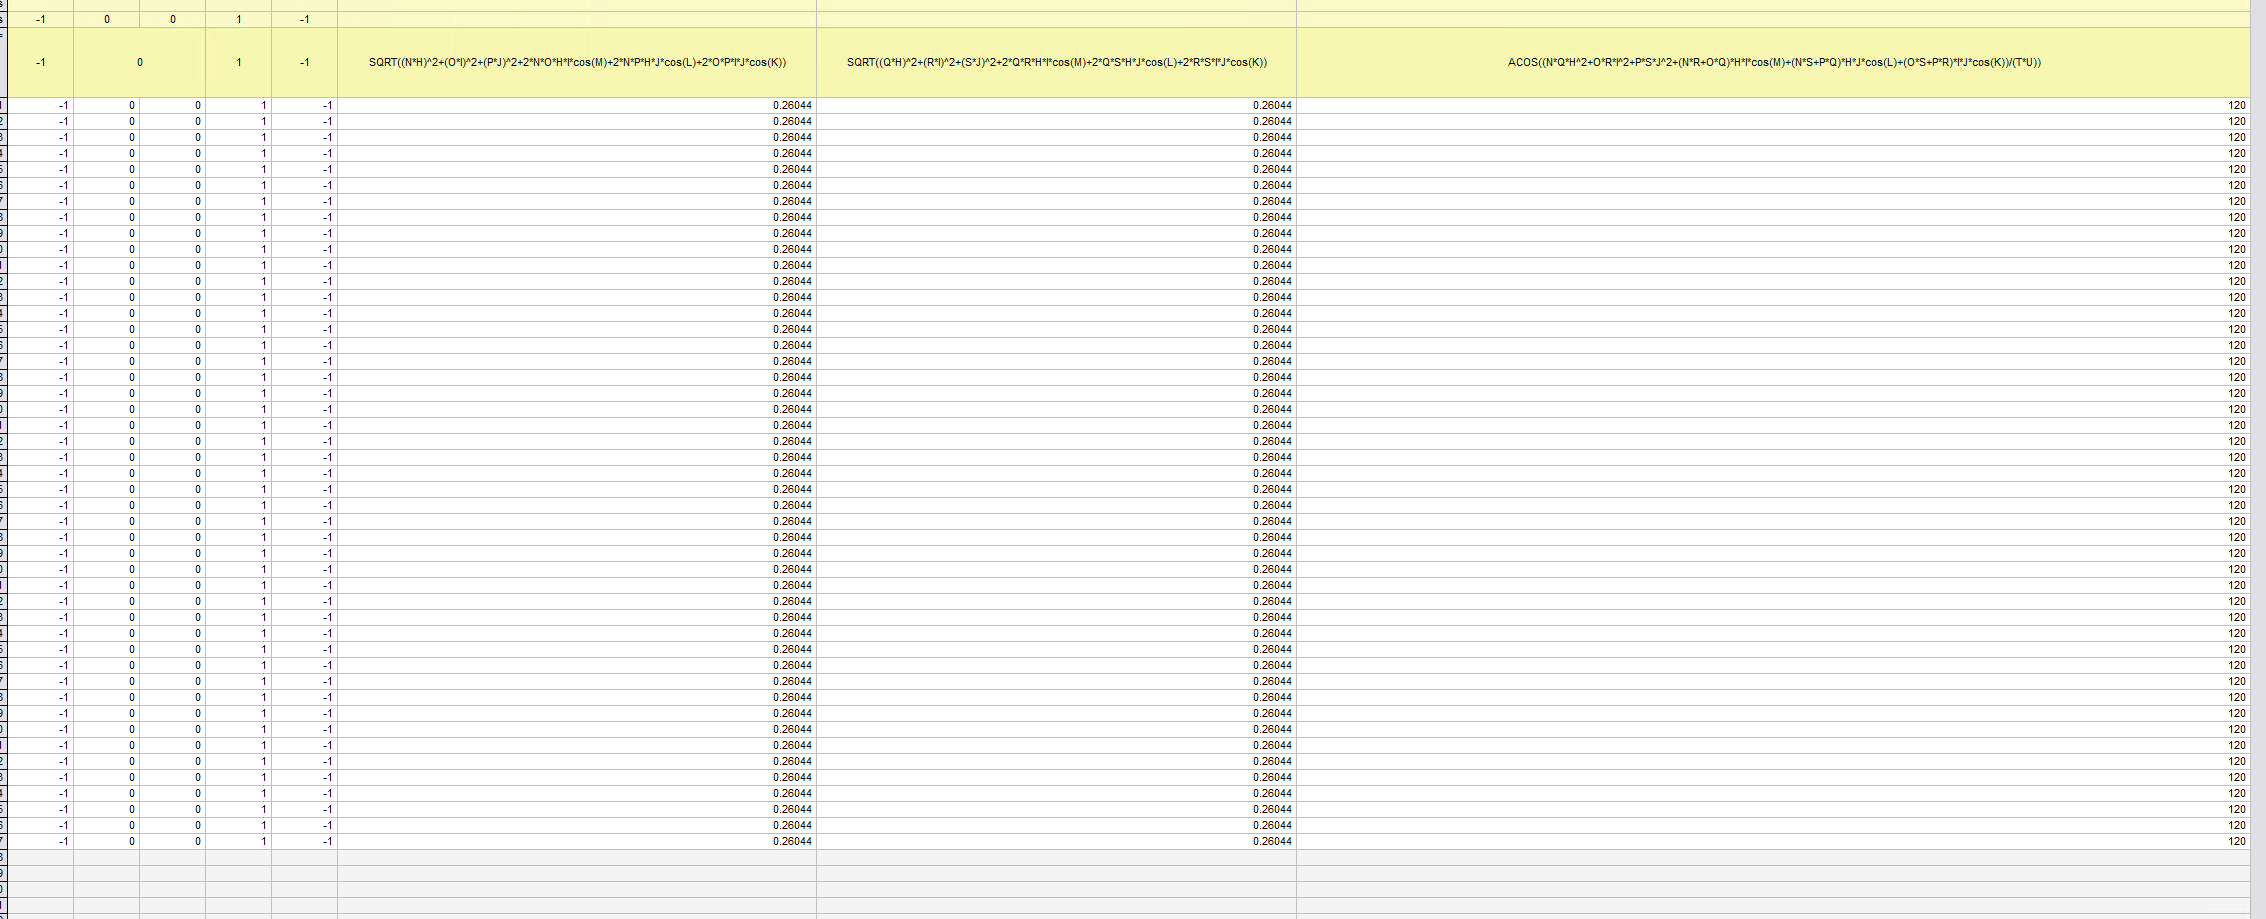
\includegraphics[width=\linewidth]{zone111/zone111_a.png}
    \caption{基矢与 $r_1,r_2,\theta$}
    \label{fig:zone111-a}
  \end{subfigure}\hfill
  \begin{subfigure}[t]{0.14\linewidth}
    \centering
    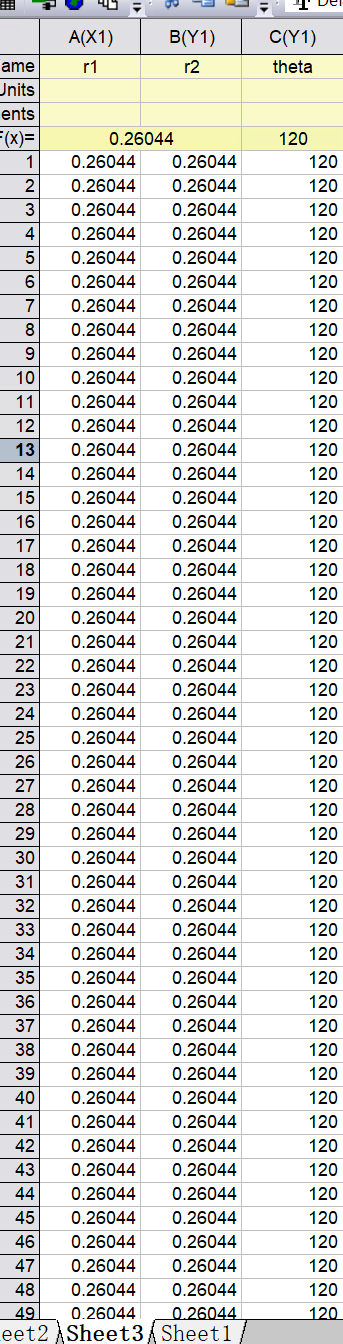
\includegraphics[height=4.3cm]{zone111/zone111_b.png}
    \caption{坐标复制}
    \label{fig:zone111-b}
  \end{subfigure}

  \vspace{0.3em}
  \begin{subfigure}[t]{0.48\linewidth}
    \centering
    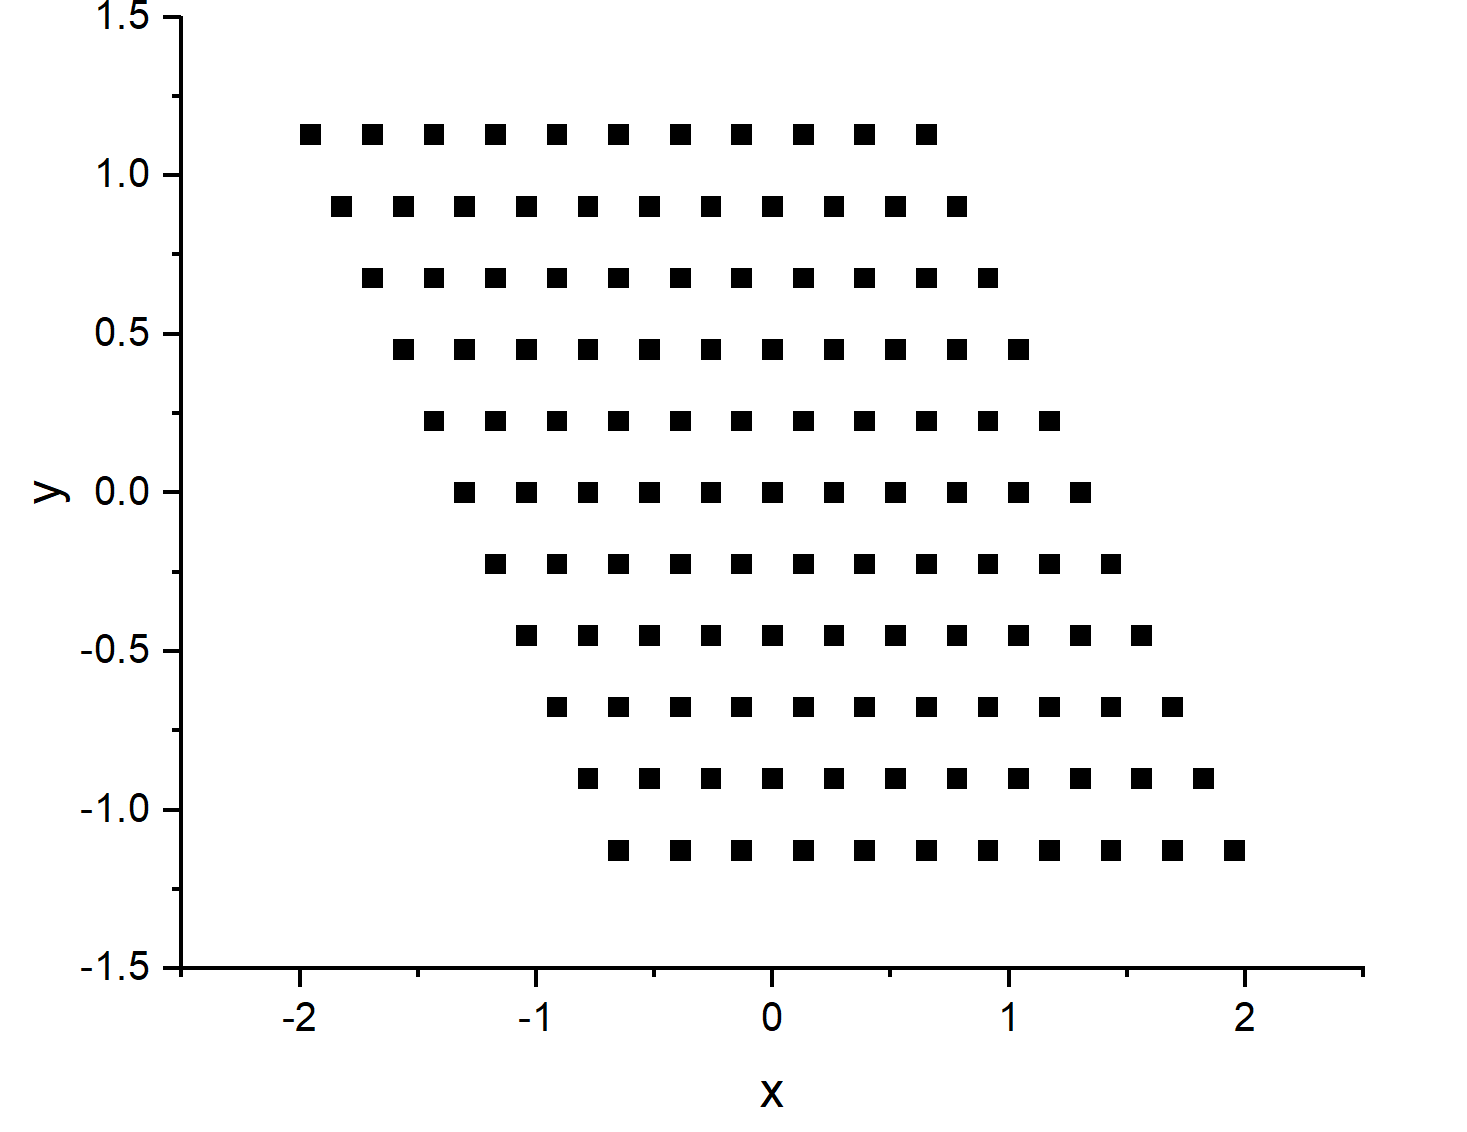
\includegraphics[width=\linewidth]{zone111/zone111_c.png}
    \caption{二维散点图}
    \label{fig:zone111-c}
  \end{subfigure}\hfill
  \begin{subfigure}[t]{0.48\linewidth}
    \centering
    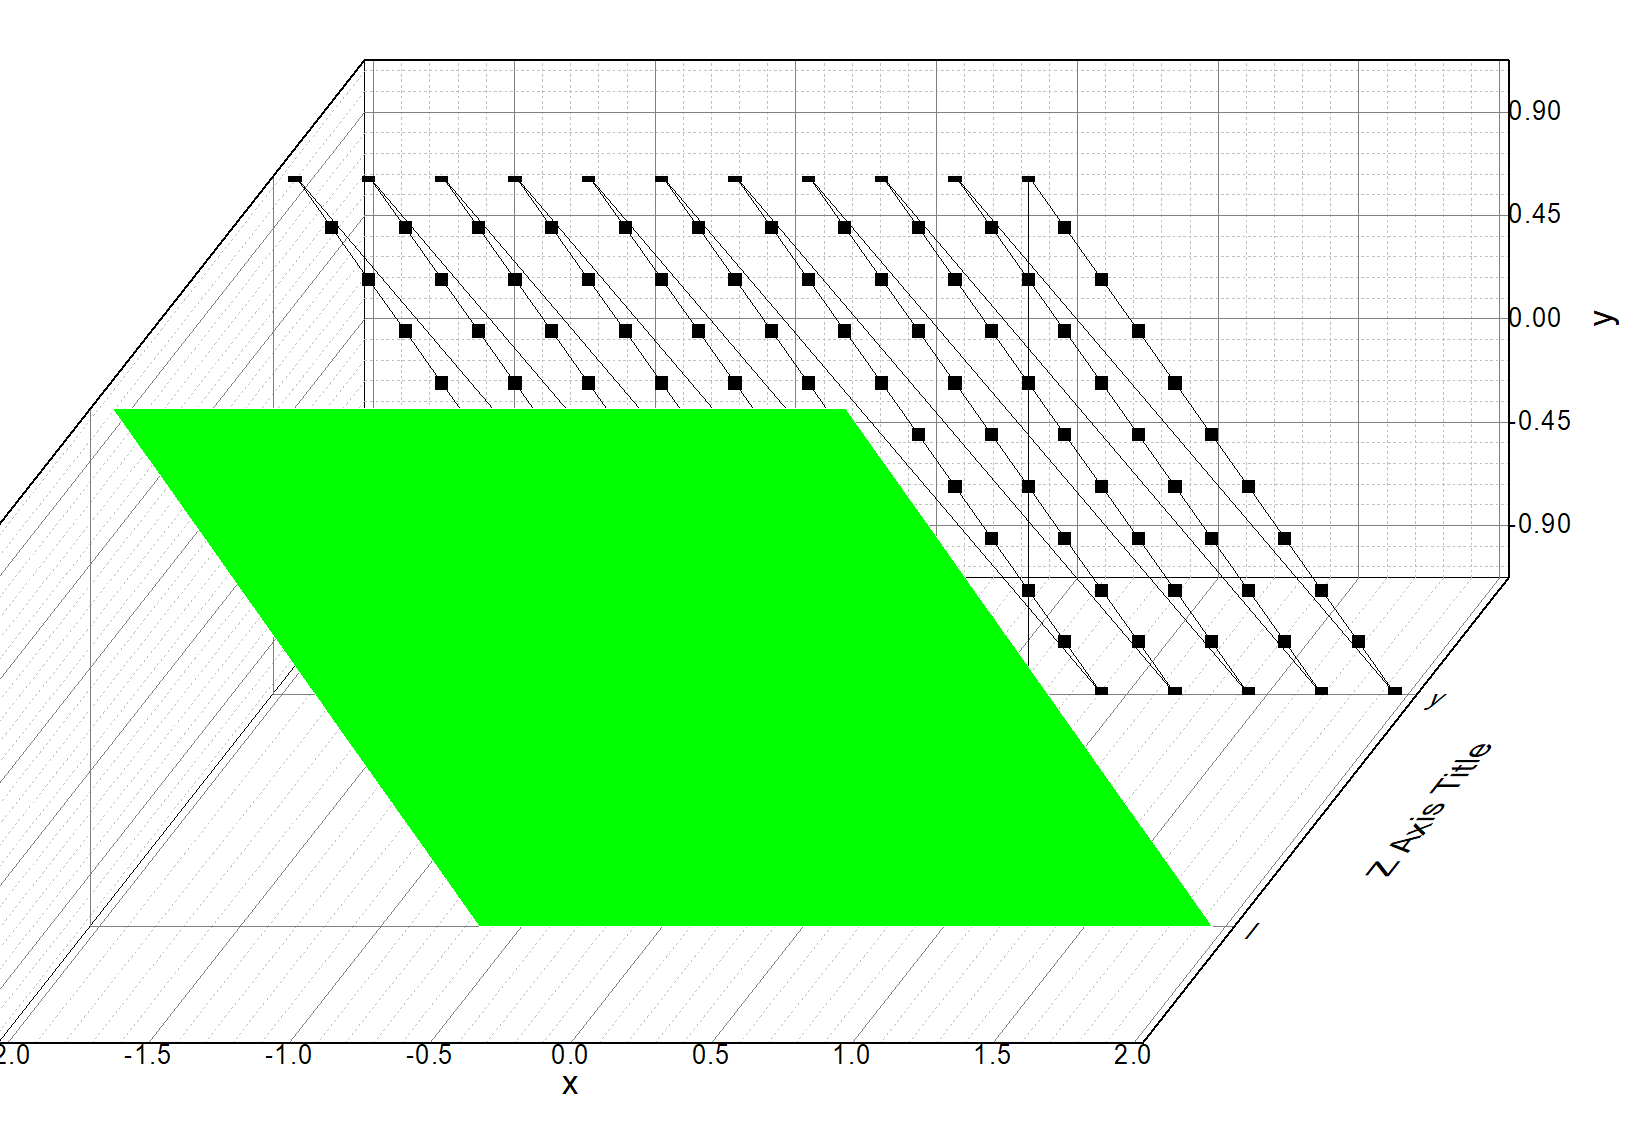
\includegraphics[width=\linewidth]{zone111/zone111_d.png}
    \caption{三维 Waterfall 图}
    \label{fig:zone111-d}
  \end{subfigure}
  \caption{[111] 带轴电子衍射模拟：(a) 基矢 $(\bar{1}01)^*$、$(0\bar{1}1)^*$ 与 $r_1=r_2=0.26044$~\AA$^{-1}$、$\theta=120^\circ$；(b) 坐标复制；(c) 三角/六方二维点阵；(d) 三维 Waterfall 图。}
  \label{fig:zone111}
\end{figure}

\subsubsection{[332] 带轴}

[332] 带轴的基矢为 $\bm{g}_1=(2\bar{2}0)^*$、$\bm{g}_2=(04\bar{6})^*$，$r_1=0.52089$~\AA$^{-1}$，$r_2=1.32801$~\AA$^{-1}$，$\theta=113.0935^\circ$。二维点阵为斜方/平行四边形，夹角大于 $90^\circ$；第二基矢较长，因此沿该方向的点间距较大。允许的反射包括 220、311、331、440 等。与 [001]、[111] 相比，[332] 的对称性明显降低，点阵不再具有 4 次或 6 次对称。

\begin{figure}[H]
  \centering
  \begin{subfigure}[t]{0.64\linewidth}
    \centering
    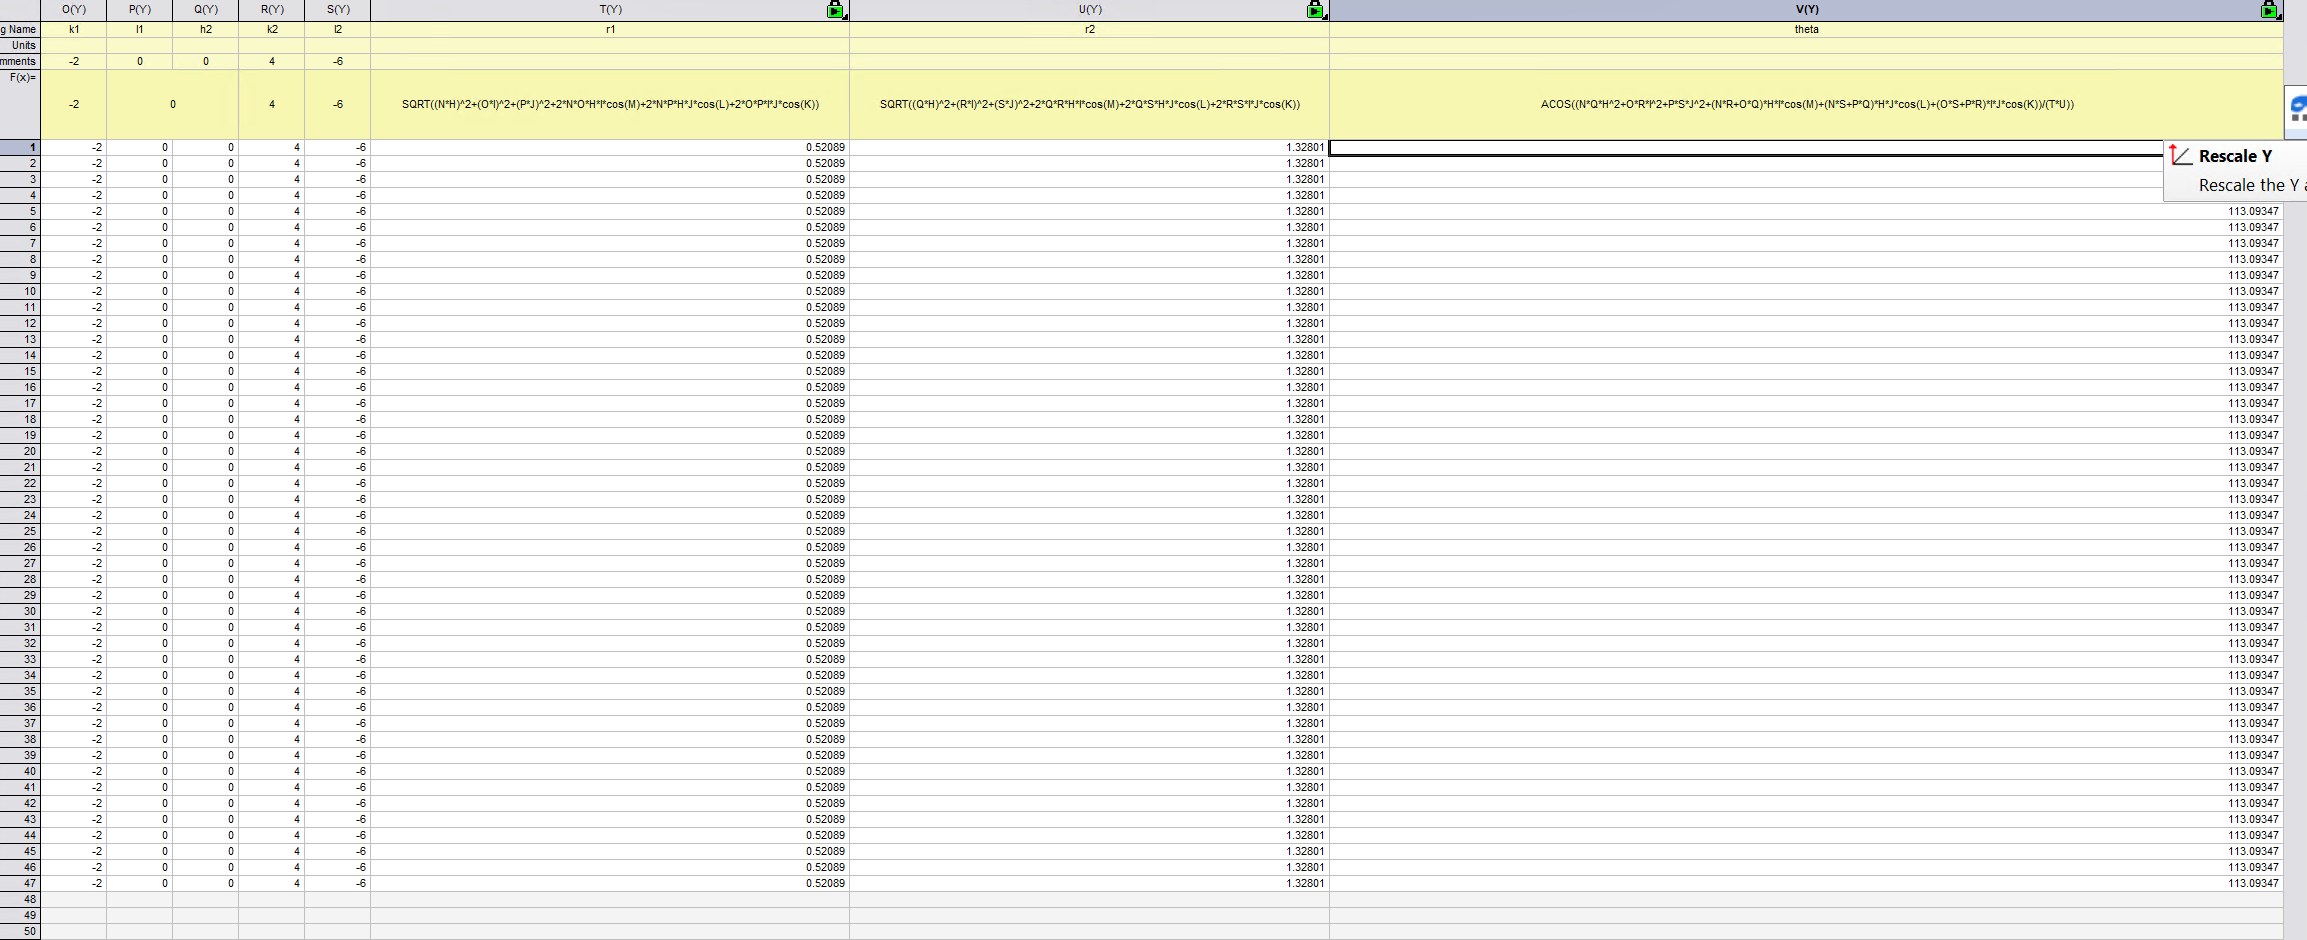
\includegraphics[width=\linewidth]{zone332/zone332_a.png}
    \caption{基矢与 $r_1,r_2,\theta$}
    \label{fig:zone332-a}
  \end{subfigure}\hfill
  \begin{subfigure}[t]{0.14\linewidth}
    \centering
    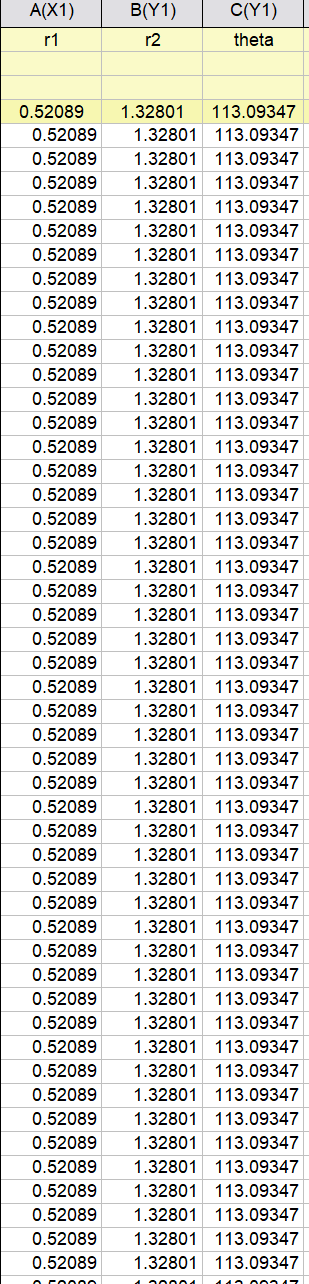
\includegraphics[height=4.3cm]{zone332/zone332_b.png}
    \caption{坐标复制}
    \label{fig:zone332-b}
  \end{subfigure}

  \vspace{0.3em}
  \begin{subfigure}[t]{0.48\linewidth}
    \centering
    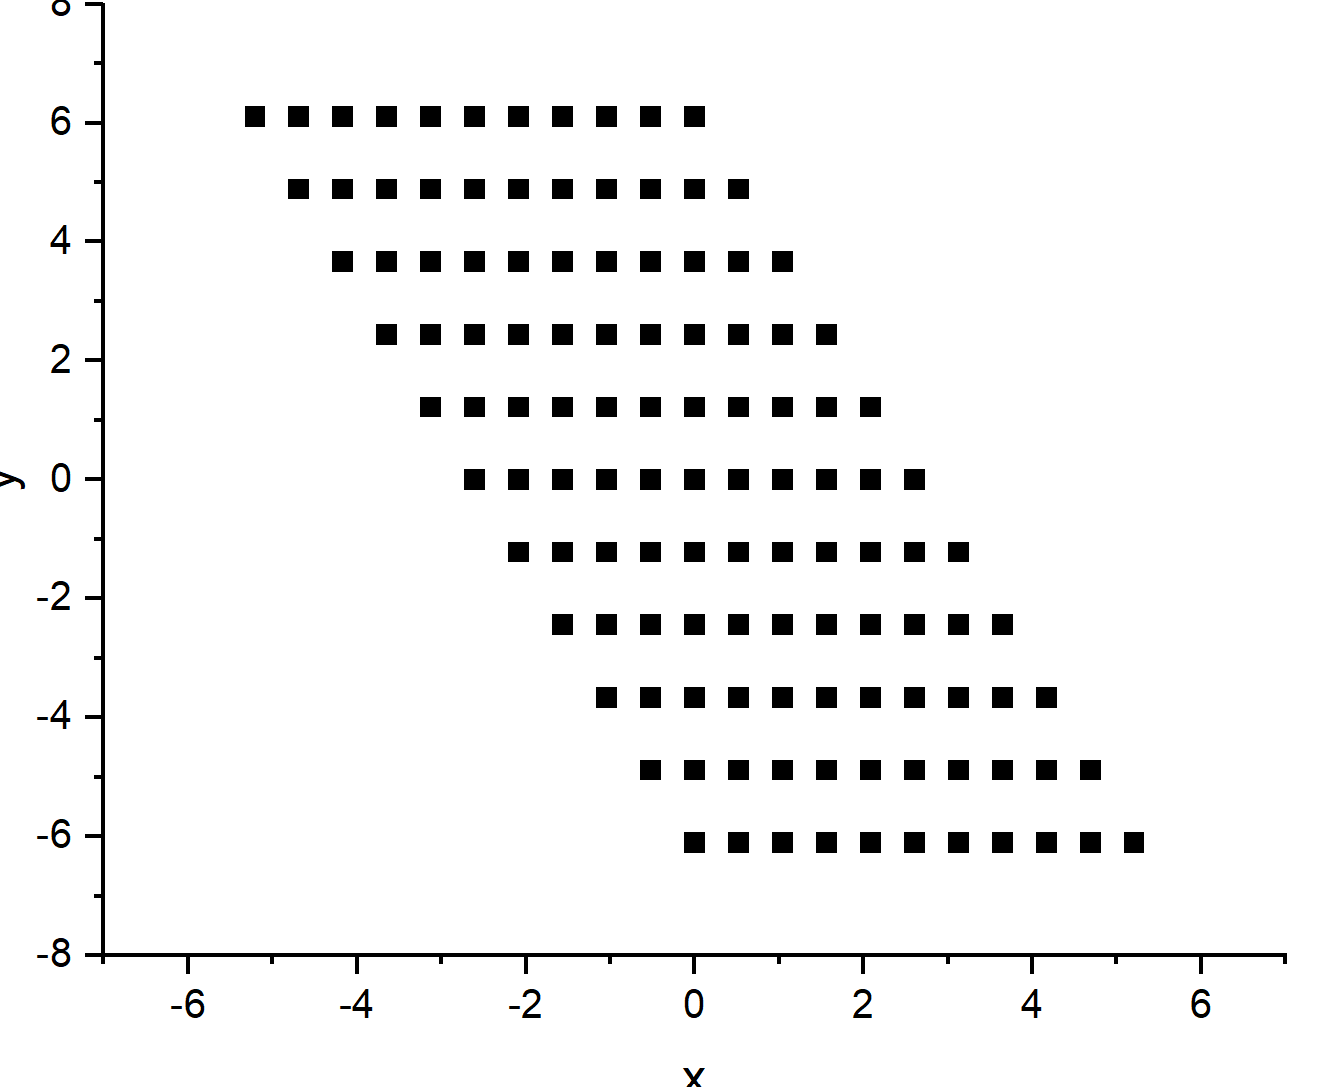
\includegraphics[width=\linewidth]{zone332/zone332_c.png}
    \caption{二维散点图}
    \label{fig:zone332-c}
  \end{subfigure}\hfill
  \begin{subfigure}[t]{0.48\linewidth}
    \centering
    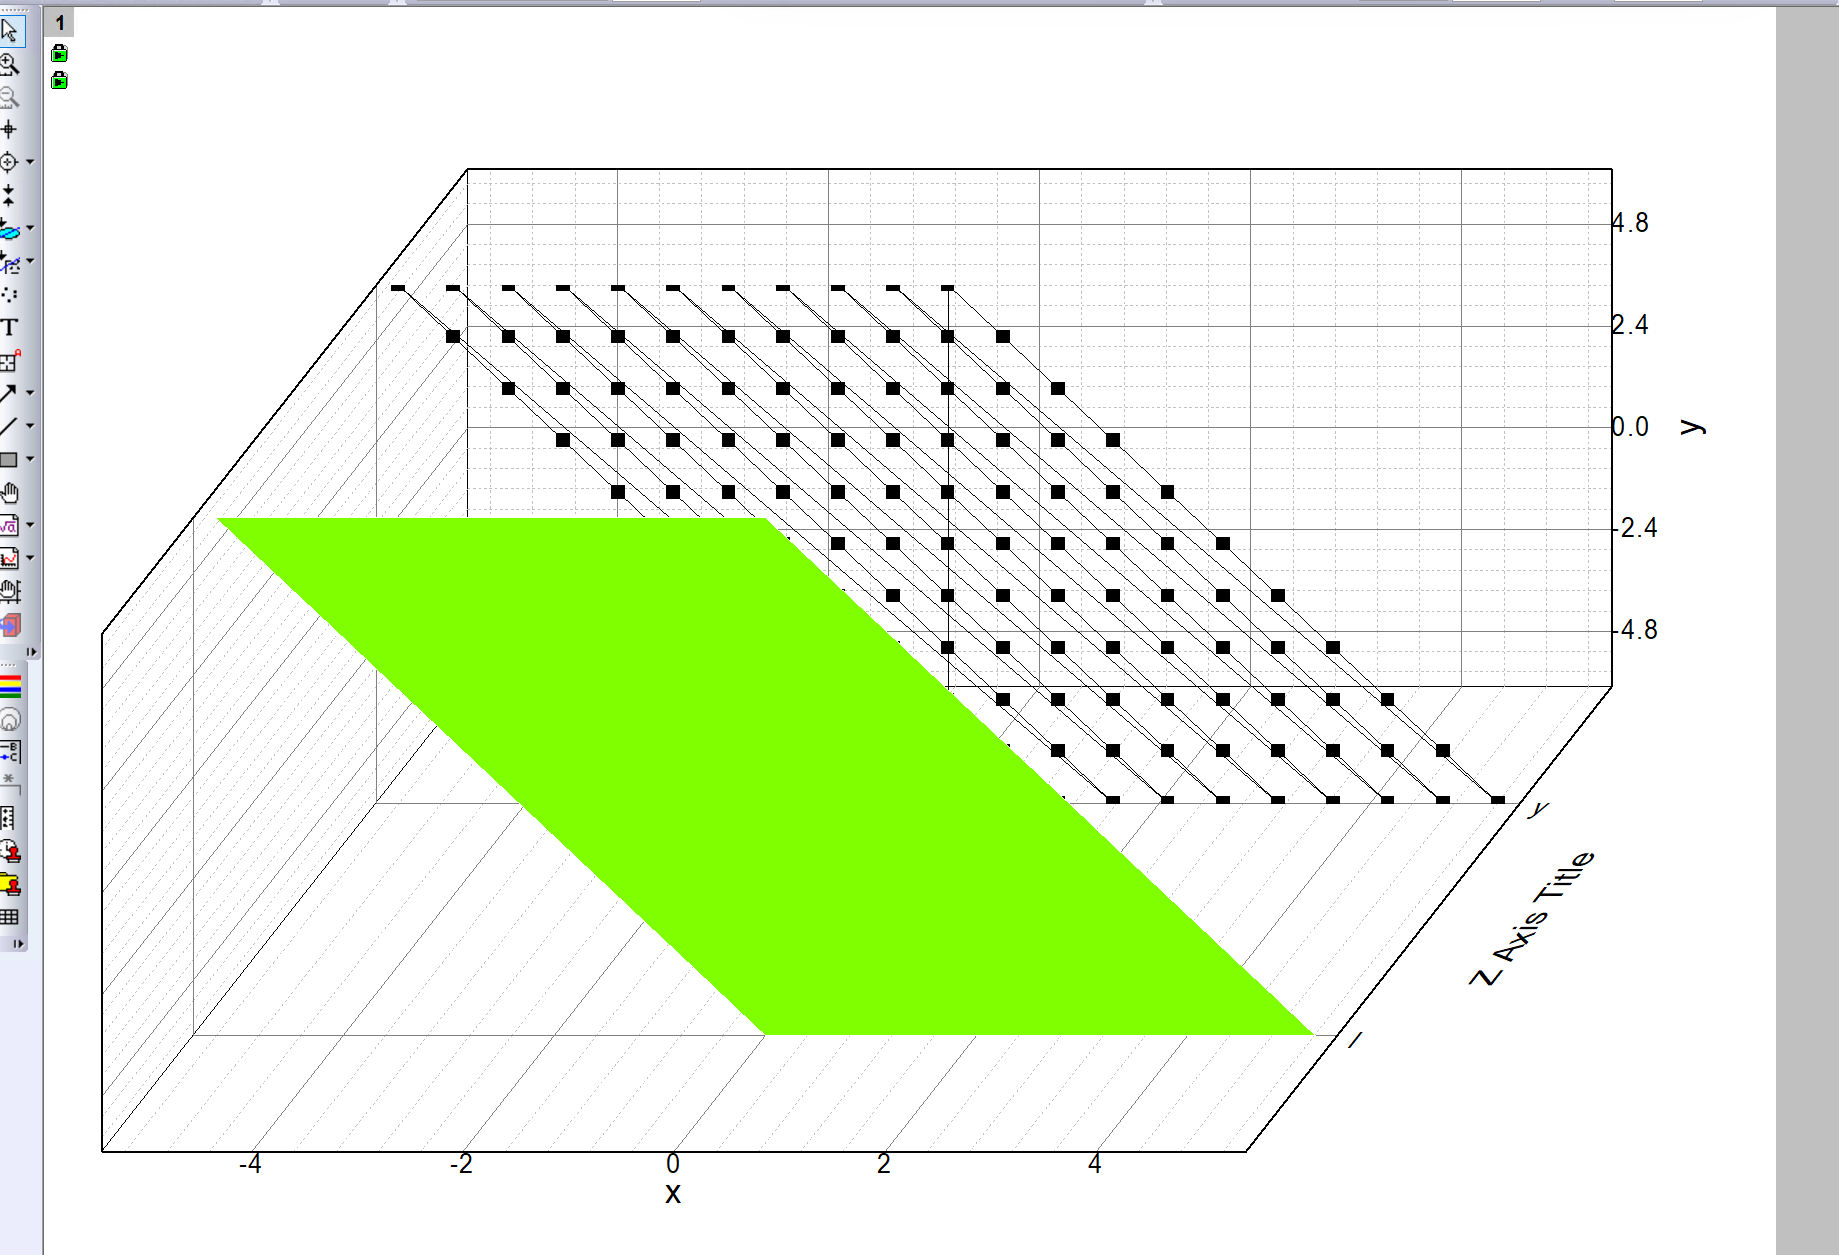
\includegraphics[width=\linewidth]{zone332/zone332_d.png}
    \caption{三维 Waterfall 图}
    \label{fig:zone332-d}
  \end{subfigure}
  \caption{[332] 带轴电子衍射模拟：(a) 基矢 $(2\bar{2}0)^*$、$(04\bar{6})^*$ 与 $r_1=0.52089$~\AA$^{-1}$、$r_2=1.32801$~\AA$^{-1}$、$\theta=113.0935^\circ$；(b) 坐标复制；(c) 斜方二维点阵；(d) 三维 Waterfall 图。}
  \label{fig:zone332}
\end{figure}

\subsubsection{[334] 带轴}

[334] 带轴的基矢为 $\bm{g}_1=(2\bar{2}0)^*$、$\bm{g}_2=(08\bar{6})^*$，$r_1=0.52089$~\AA$^{-1}$，$r_2=1.84162$~\AA$^{-1}$，$\theta=124.4499^\circ$。它与 [332] 共用 $\bm{g}_1=(2\bar{2}0)^*$，但 $\bm{g}_2$ 由 $(04\bar{6})^*$ 变为 $(08\bar{6})^*$，长度由 1.32801 增至 1.84162~\AA$^{-1}$，夹角由 $113.09^\circ$ 增至 $124.45^\circ$。因此 [334] 的点阵更“斜”，第二方向的点间距更大；允许的反射包括 220、331、440、531 等。

\begin{figure}[H]
  \centering
  \begin{subfigure}[t]{0.64\linewidth}
    \centering
    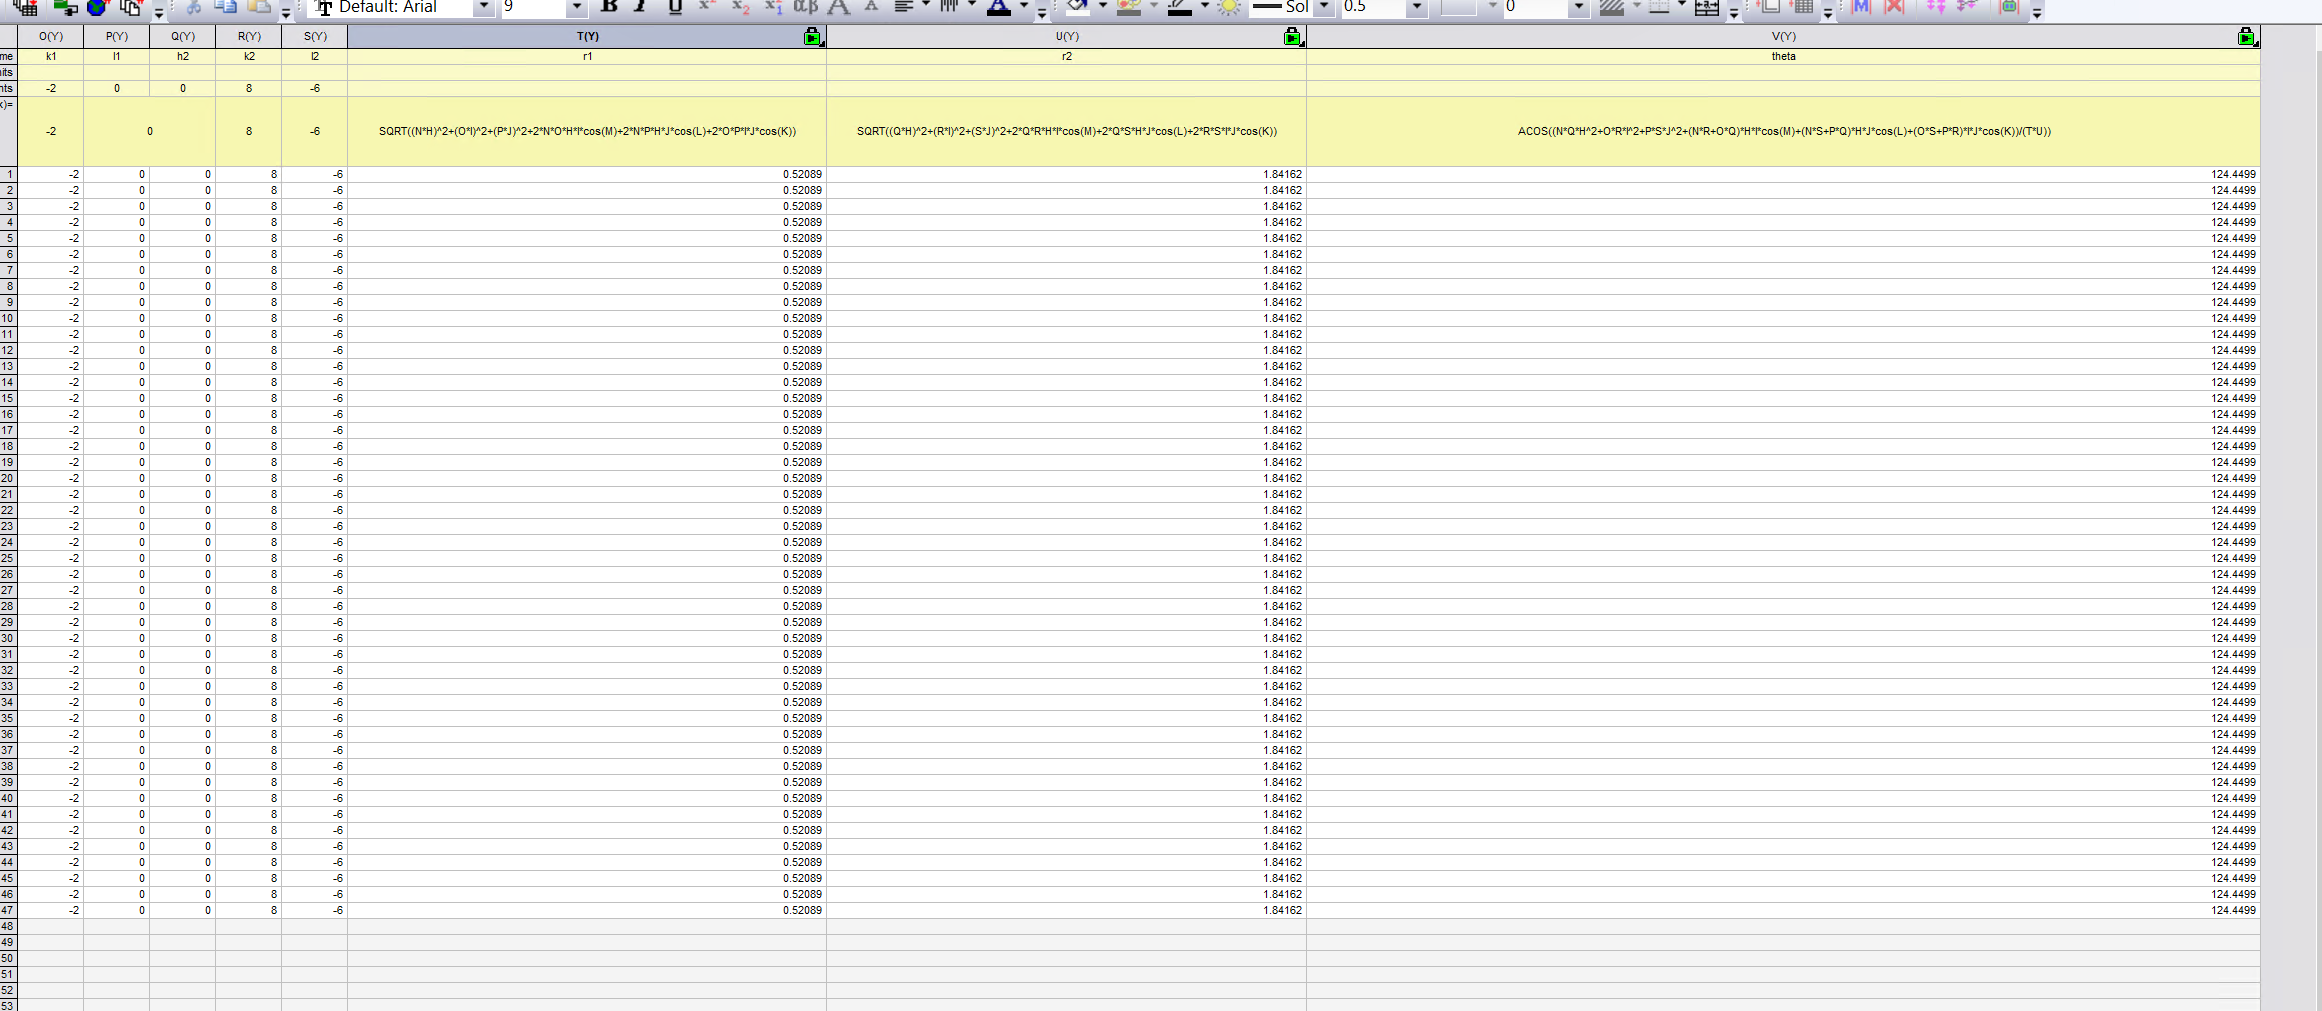
\includegraphics[width=\linewidth]{zone334/zone334_a.png}
    \caption{基矢与 $r_1,r_2,\theta$}
    \label{fig:zone334-a}
  \end{subfigure}\hfill
  \begin{subfigure}[t]{0.14\linewidth}
    \centering
    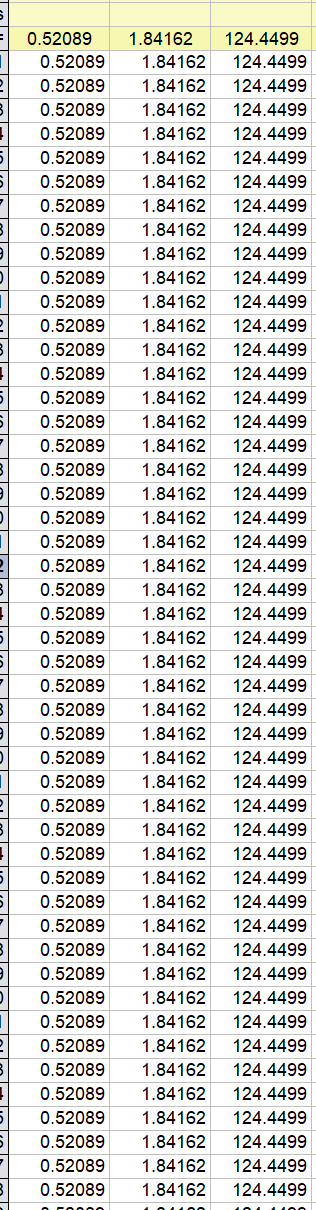
\includegraphics[height=4.3cm]{zone334/zone334_b.png}
    \caption{坐标复制}
    \label{fig:zone334-b}
  \end{subfigure}

  \vspace{0.3em}
  \begin{subfigure}[t]{0.48\linewidth}
    \centering
    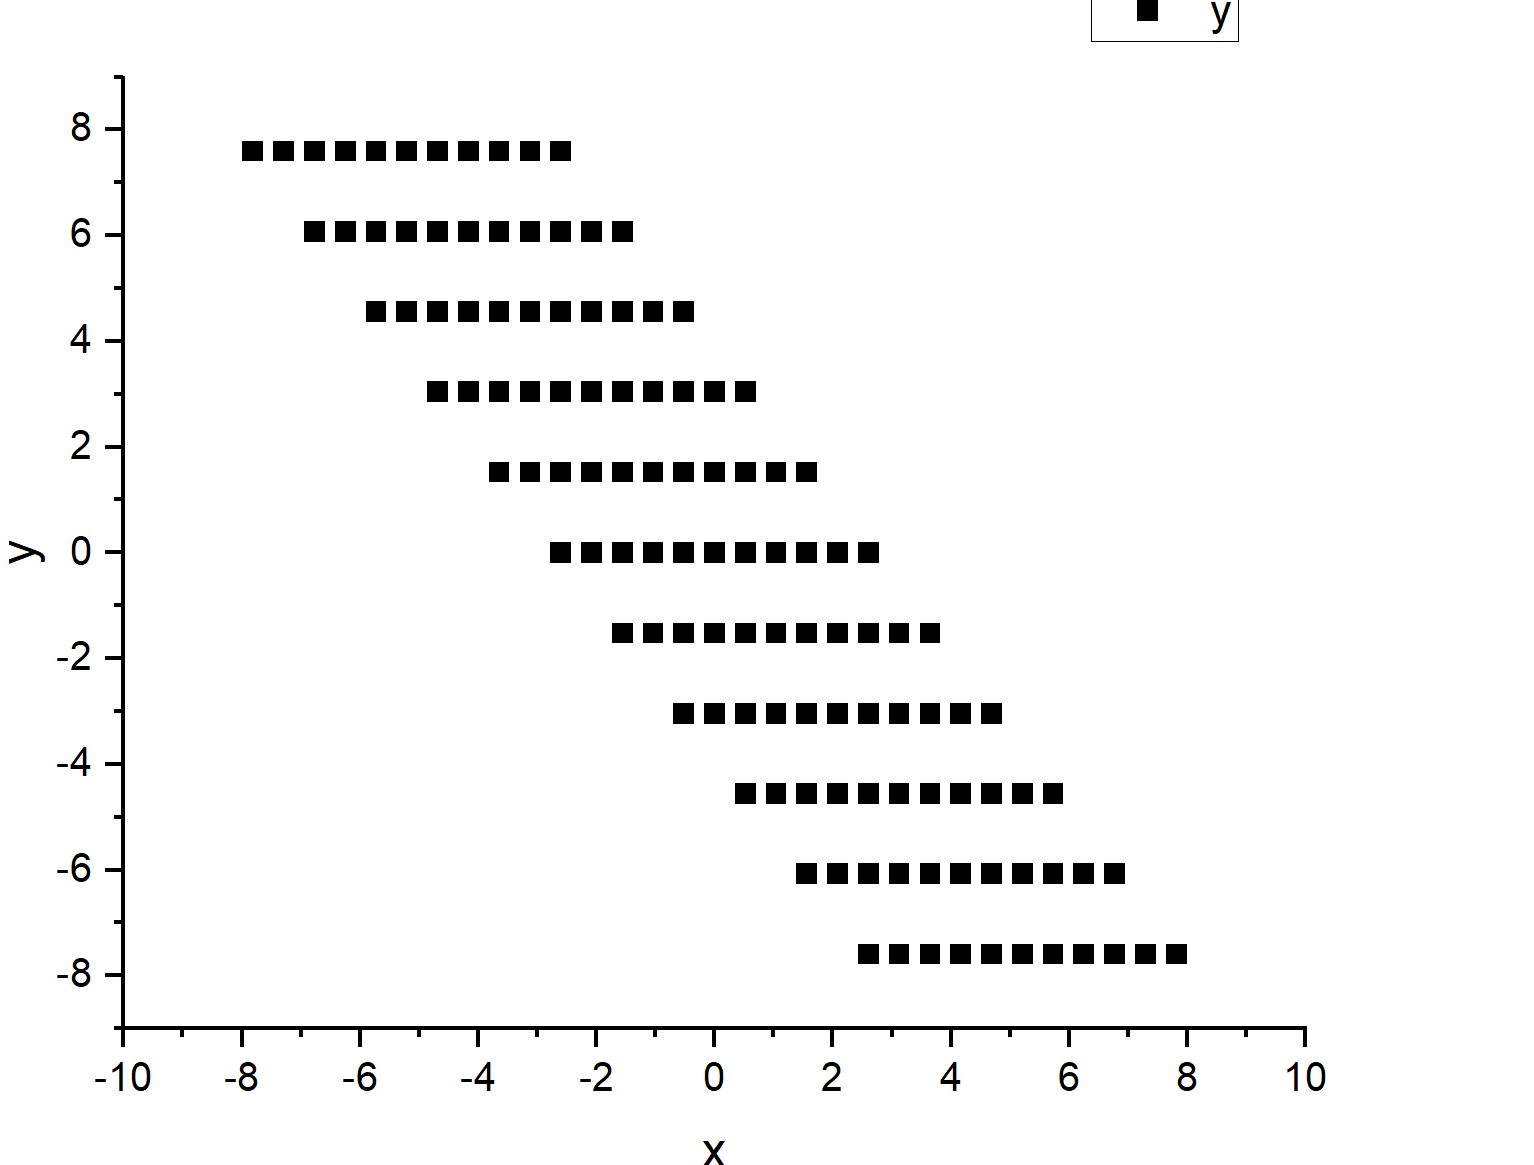
\includegraphics[width=\linewidth]{zone334/zone334_c.png}
    \caption{二维散点图}
    \label{fig:zone334-c}
  \end{subfigure}\hfill
  \begin{subfigure}[t]{0.48\linewidth}
    \centering
    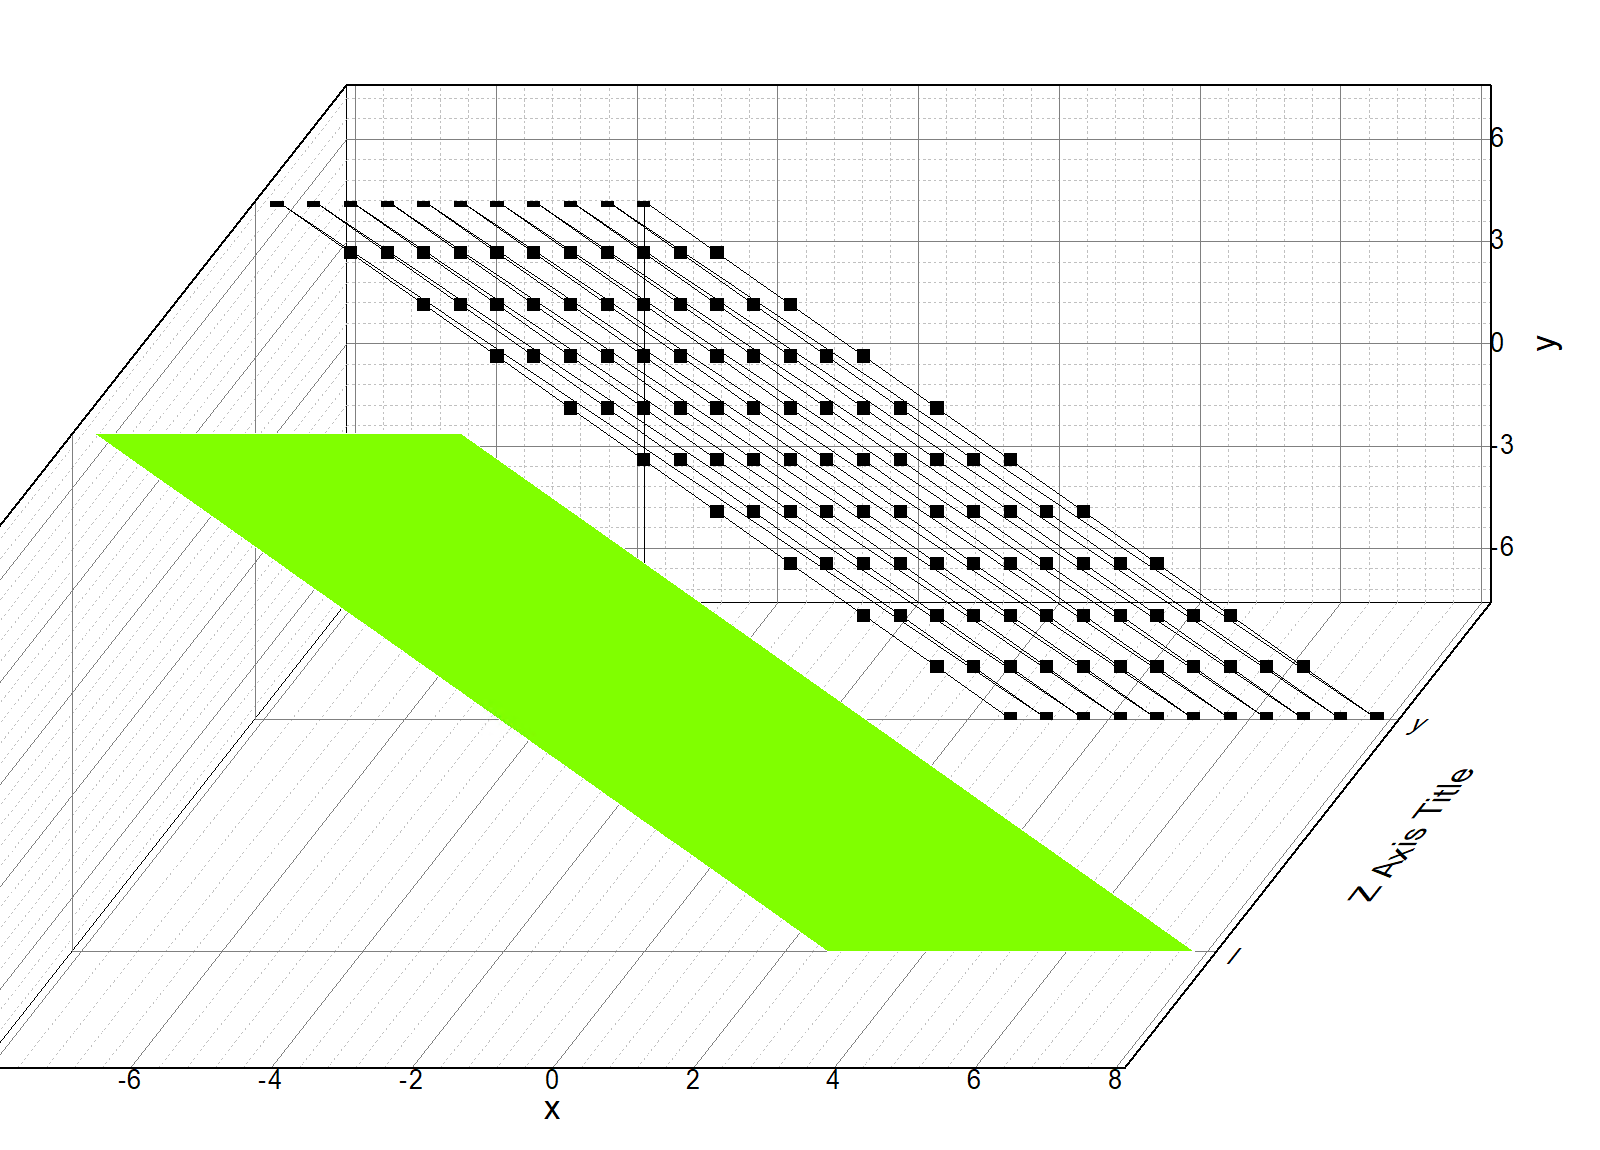
\includegraphics[width=\linewidth]{zone334/zone334_d.png}
    \caption{三维 Waterfall 图}
    \label{fig:zone334-d}
  \end{subfigure}
  \caption{[334] 带轴电子衍射模拟：(a) 基矢 $(2\bar{2}0)^*$、$(08\bar{6})^*$ 与 $r_1=0.52089$~\AA$^{-1}$、$r_2=1.84162$~\AA$^{-1}$、$\theta=124.4499^\circ$；(b) 坐标复制；(c) 斜方二维点阵；(d) 三维 Waterfall 图。}
  \label{fig:zone334}
\end{figure}

\subsubsection{[345] 带轴}

[345] 带轴的基矢为 $\bm{g}_1=(2\bar{4}2)^*$、$\bm{g}_2=(\bar{6}22)^*$，$r_1=0.90221$~\AA$^{-1}$，$r_2=1.22159$~\AA$^{-1}$，$\theta=119.4962^\circ$。这是五个带轴中指数最高、对称性最低的一个；$r_1$ 明显大于 [001] 和 [111]，因此视场内点数较少、点间距较大。允许的反射包括 311、331、422、531 等。图 \ref{fig:zone345}(c) 的二维点阵呈明显的斜方排列，图 \ref{fig:zone345}(d) 的三维 Waterfall 图也反映了同样的几何。

\begin{figure}[H]
  \centering
  \begin{subfigure}[t]{0.64\linewidth}
    \centering
    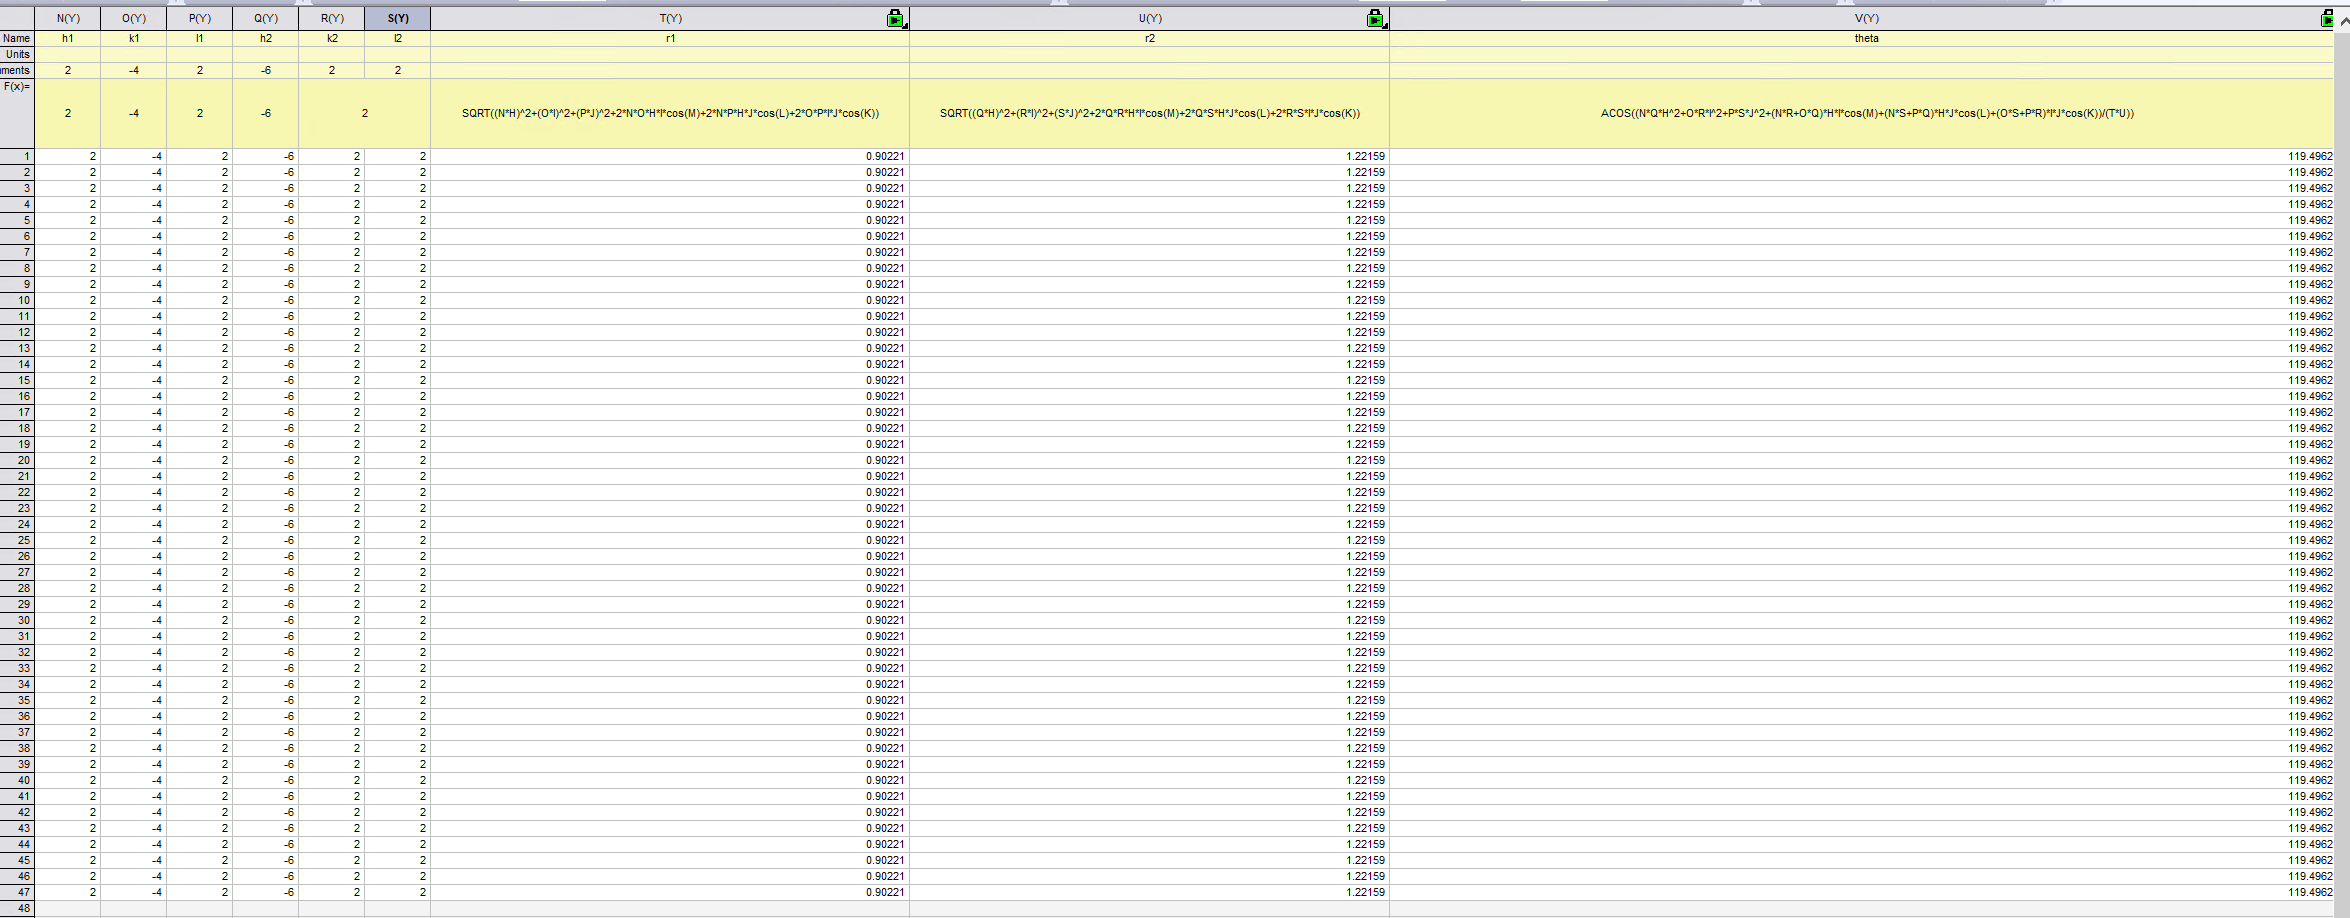
\includegraphics[width=\linewidth]{zone345/zone345_a.png}
    \caption{基矢与 $r_1,r_2,\theta$}
    \label{fig:zone345-a}
  \end{subfigure}\hfill
  \begin{subfigure}[t]{0.14\linewidth}
    \centering
    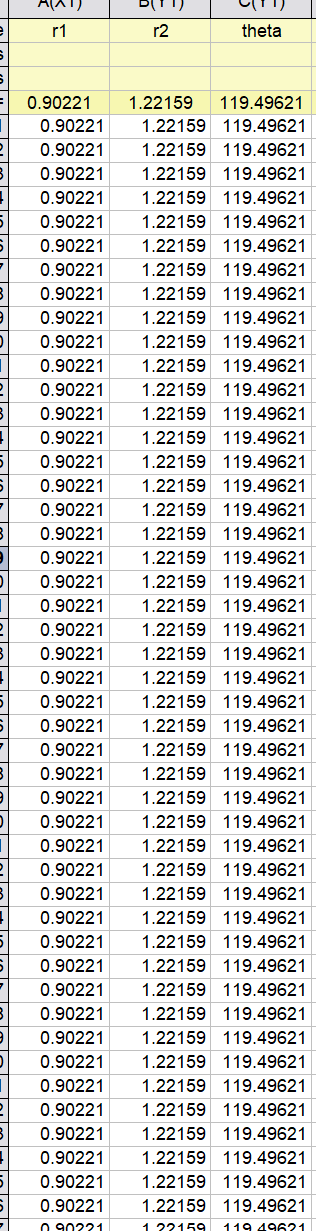
\includegraphics[height=4.3cm]{zone345/zone345_b.png}
    \caption{坐标复制}
    \label{fig:zone345-b}
  \end{subfigure}

  \vspace{0.3em}
  \begin{subfigure}[t]{0.48\linewidth}
    \centering
    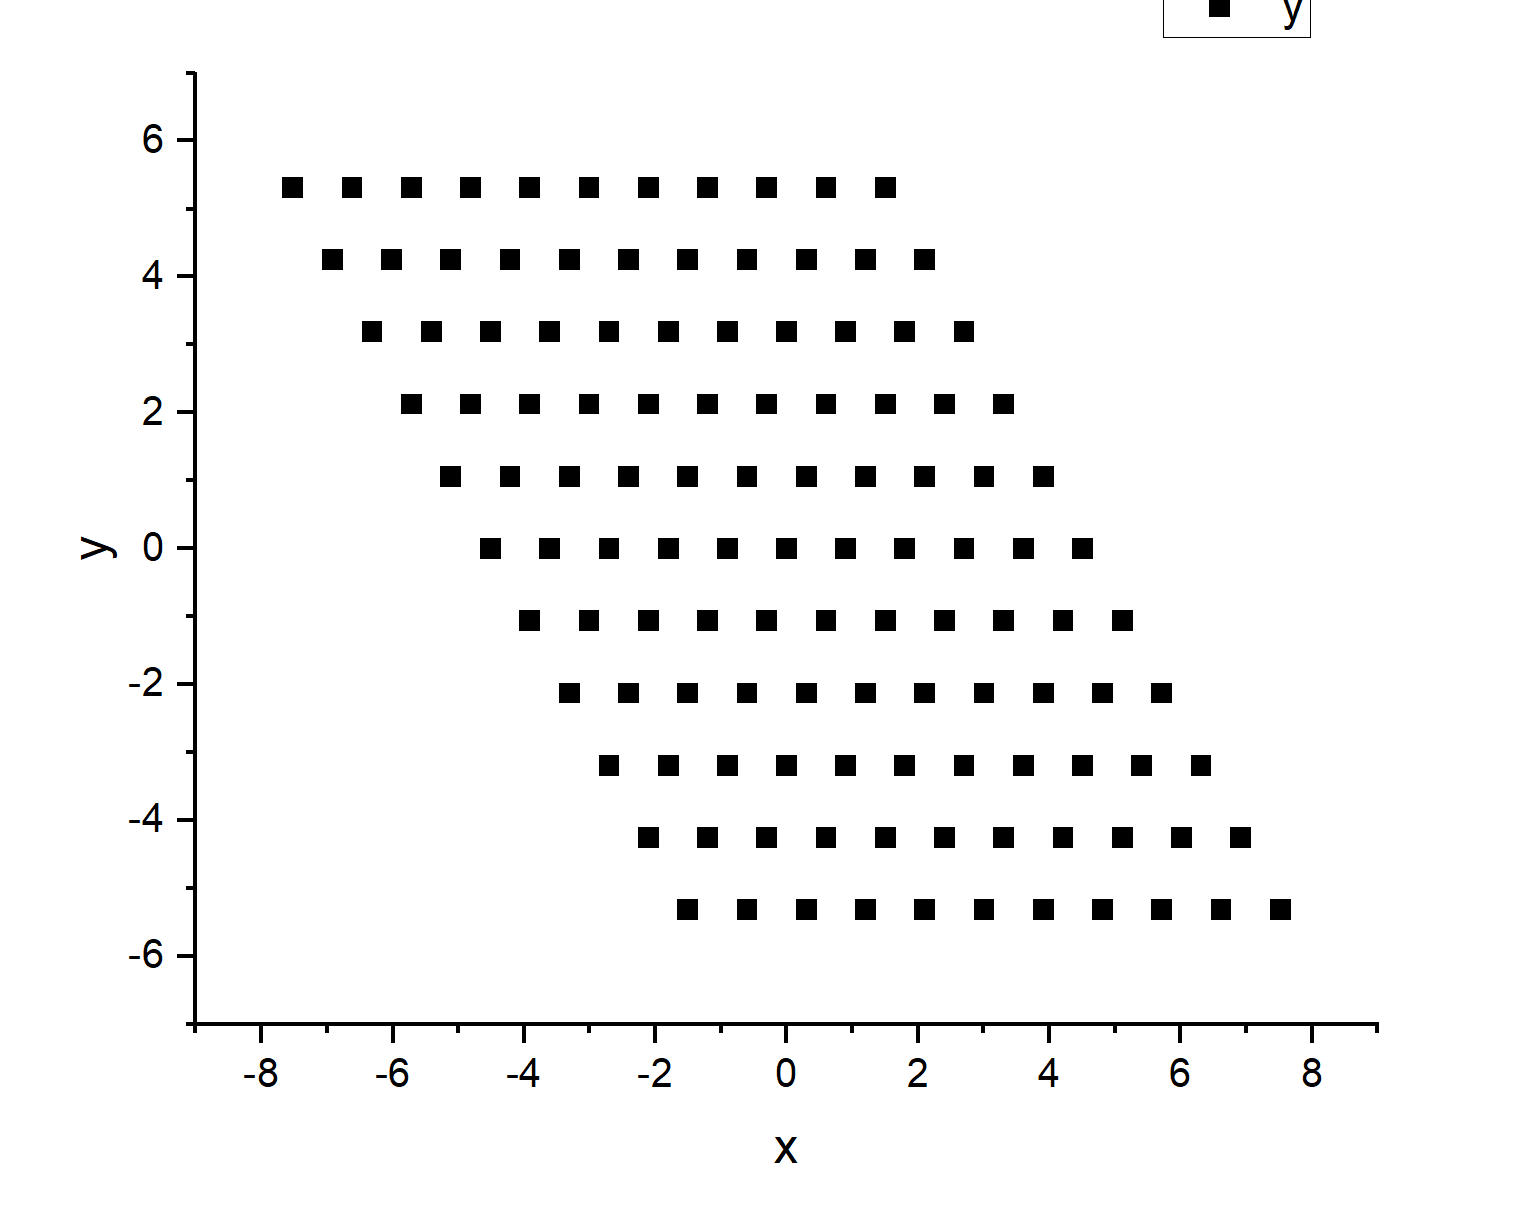
\includegraphics[width=\linewidth]{zone345/zone345_c.png}
    \caption{二维散点图}
    \label{fig:zone345-c}
  \end{subfigure}\hfill
  \begin{subfigure}[t]{0.48\linewidth}
    \centering
    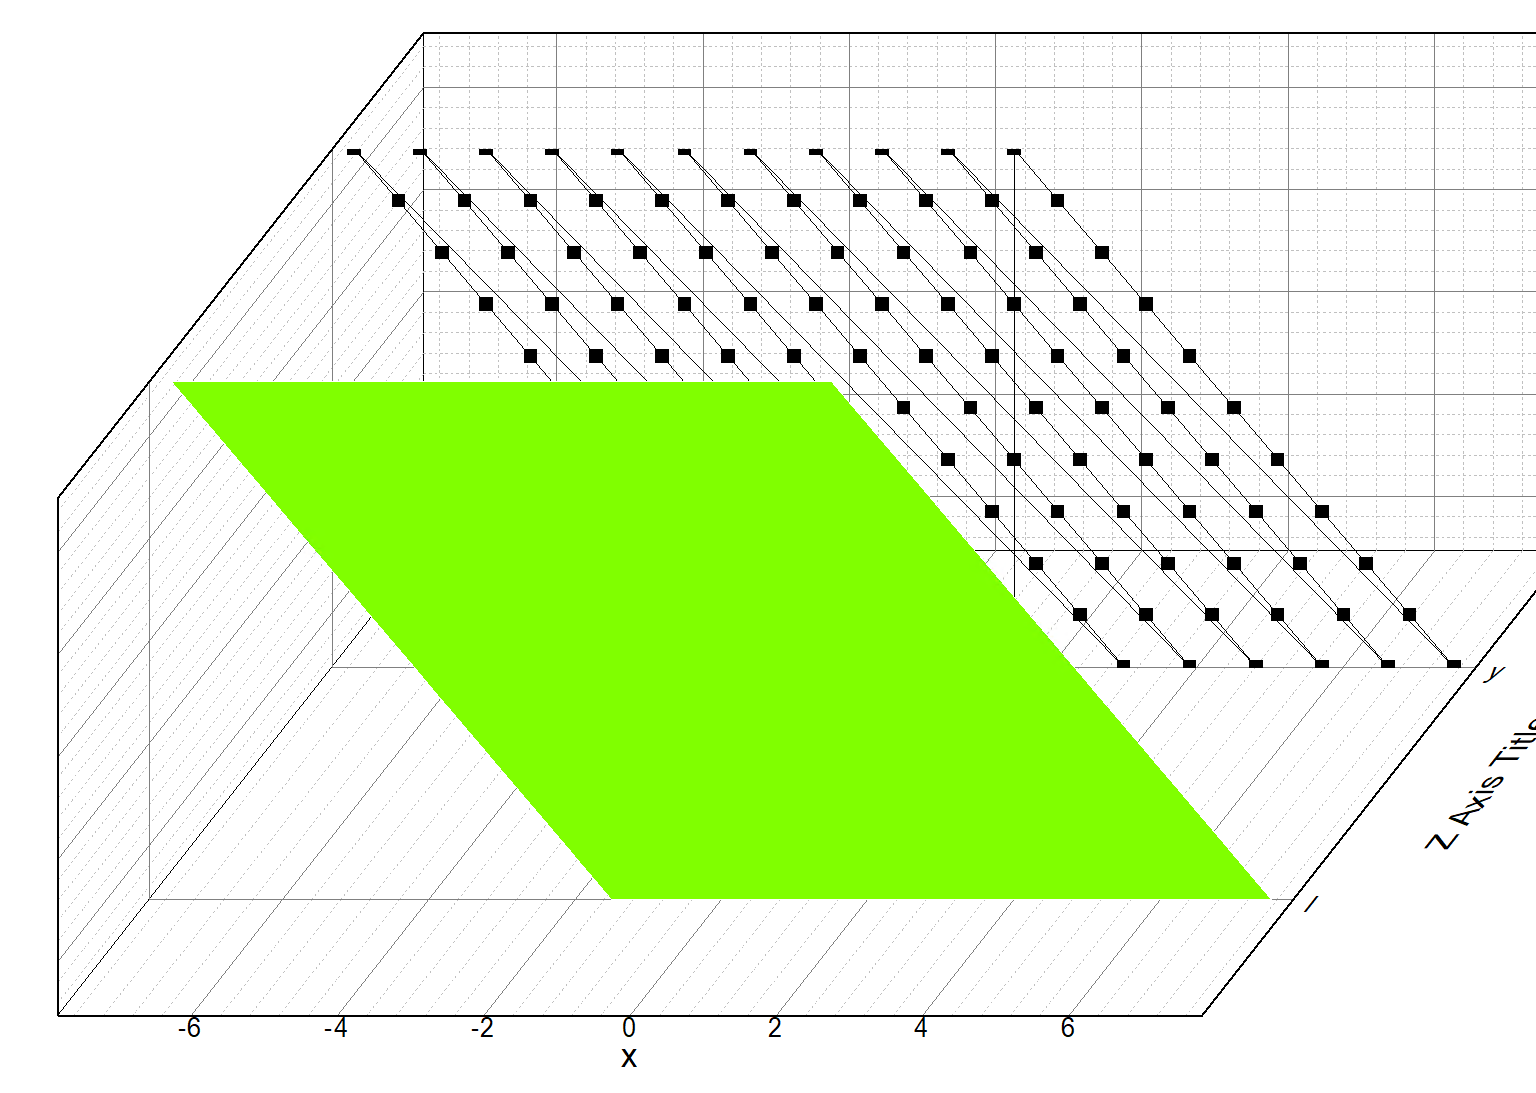
\includegraphics[width=\linewidth]{zone345/zone345_d.png}
    \caption{三维 Waterfall 图}
    \label{fig:zone345-d}
  \end{subfigure}
  \caption{[345] 带轴电子衍射模拟：(a) 基矢 $(2\bar{4}2)^*$、$(\bar{6}22)^*$ 与 $r_1=0.90221$~\AA$^{-1}$、$r_2=1.22159$~\AA$^{-1}$、$\theta=119.4962^\circ$；(b) 坐标复制；(c) 斜方二维点阵；(d) 三维 Waterfall 图。}
  \label{fig:zone345}
\end{figure}

\subsection{讨论}

把五个带轴放在一起比较，可以看到一条清晰的规律：带轴指数越低、对称性越高，二维点阵越规整；带轴指数越高，点阵越“斜”，点间距和夹角越不规整。表 \ref{tab:zone-summary} 汇总了五个带轴的几何参数、点阵类型和代表反射。[001] 是正方形点阵，[111] 是三角/六方点阵，这两个低指数带轴具有最高的对称性；[332] 和 [334] 共用 $\bm{g}_1=(2\bar{2}0)^*$，但第二条基矢不同，因此一个方向的点间距相同、另一个方向的点间距和夹角不同；[345] 的两条基矢都较长，视场内点数最少，斜方特征最明显。

从衍射强度的角度看，几何点阵只给出“可能出现”的位置，真正“出现”的斑点还要满足结构因子不为零。第 3 章的 110 消光计算（图 \ref{fig:extinction}）就是一个典型例子：它在几何点阵中有确定的位置，但 $h,k,l$ 奇偶混合使 $F=0$，强度在数值上为零。对单晶硅，实际允许的反射是 111、220、311、400、331、422、511/333、440 等；在 [001] 带轴中，100、110、200 等消光，220、400 等出现；在 [111] 带轴中，111 属于高阶劳厄带，零阶劳厄区内的强点是 220、422、440 等。

本模拟还有几点局限。第一，采用运动学近似，忽略了电子衍射的动力学效应（多次散射、厚度消光等），因此强点的相对强度只能作半定量参考。第二，结构因子计算取 $f=14$ 的常数原子散射因子，没有考虑 $f(s)$ 随角度的衰减和温度因子；若需要更接近实验的强度，可按式 \eqref{eq:cromer-mann} 把 $f$ 换成 $f(s)$，并加入 Debye--Waller 因子。第三，所选基矢不一定是最短的二维基矢，例如 [332] 的 $\bm{g}_2=(04\bar{6})^*$ 是 $(02\bar{3})^*$ 的两倍；若取最短基矢或允许 $m,n$ 取半整数，可以得到更完整的倒易点阵。第四，模拟中没有相机长度、比例尺和 HOLZ 线，实际 SAED 花样的标定还需要相机常数和仪器参数。尽管有这些简化，五个带轴的模拟结果已经能够正确反映点阵几何、对称性和消光规律，达到了预期的模拟效果。

\begin{table}[H]
  \centering
  \caption{五个带轴的点阵特征与代表反射汇总}
  \label{tab:zone-summary}
  \small
  \setlength{\tabcolsep}{4pt}
  \renewcommand{\arraystretch}{1.08}
  \begin{tabular}{cccccl}
    \toprule
    带轴 & $r_1$/\AA$^{-1}$ & $r_2$/\AA$^{-1}$ & $\theta$/$^\circ$ & 点阵 & 代表允许反射 \\
    \midrule
    {}[001] & 0.18416 & 0.18416 & 90.0000  & 正方 & 220, 400, 440, 620 \\
    {}[111] & 0.26044 & 0.26044 & 120.0000 & 三角/六方 & 220, 422, 440 \\
    {}[332] & 0.52089 & 1.32801 & 113.0935 & 斜方 & 220, 311, 331, 440 \\
    {}[334] & 0.52089 & 1.84162 & 124.4499 & 斜方 & 220, 331, 440, 531 \\
    {}[345] & 0.90221 & 1.22159 & 119.4962 & 斜方 & 311, 331, 422, 531 \\
    \bottomrule
  \end{tabular}
\end{table}

% ==================== 5 结论 ====================
\section{结\hspace{0.5em}论}

本文以单晶硅为对象，完成了晶体学计算模板的建立、PDF 卡片的构建、晶面消光系数的计算和五个带轴电子衍射的模拟，主要结果如下。

（1）在 Origin 中建立了一套可复用的晶体学计算模板。模板以 A--F 列输入 $a,b,c,\alpha,\beta,\gamma$，以 G 列计算晶胞体积，以 H--M 列计算倒易点阵参数，以 N--S 列输入两组晶面指数，以 T--V 列计算倒易矢量长度 $r_1,r_2$ 和夹角 $\theta$。对 $a=5.43$~\AA 的单晶硅，模板给出 $V=160.103$~\AA$^3$、$a^*=b^*=c^*=0.18416$~\AA$^{-1}$、$\alpha^*=\beta^*=\gamma^*=90^\circ$，与立方晶系的解析结果一致。

（2）在模板基础上增加了 $2\theta$、多重性、$|F|^2$ 和相对强度四列，构建了单晶硅 PDF 卡片。Cu K$\alpha_1$ 条件下最强的衍射线为 111（$2\theta=28.45^\circ$），其次是 220（$47.31^\circ$）、311（$56.13^\circ$）、422（$88.05^\circ$）等；高角反射的强度对原子散射因子 $f(s)$ 和温度因子很敏感，说明 PDF 卡片的强度计算不能只用常数 $f$。

（3）先由 VESTA 导出的 8 个原子坐标和结构因子计算晶面的消光系数，判断允许/消光；再用晶带方程选取基矢，用式 \eqref{eq:xy} 和式 \eqref{eq:hkl-mn} 建立二维点阵，完成了 [001]、[111]、[332]、[334]、[345] 五个带轴的电子衍射模拟。[001] 为正方形点阵（$r_1=r_2=0.18416$~\AA$^{-1}$，$\theta=90^\circ$），[111] 为三角/六方点阵（$r_1=r_2=0.26044$~\AA$^{-1}$，$\theta=120^\circ$），[332]、[334]、[345] 为不同夹角和间距的斜方点阵。五个带轴的基矢叉积分别平行于对应的带轴，验证了几何关系的正确性。

（4）以 110 反射为例验证了金刚石结构的消光规律。110 的 $h,k,l$ 奇偶混合，8 个原子的实部正负抵消，计算强度约为 $4.7\times10^{-29}$，在数值上为零。这说明几何点阵只给出可能出现的位置，实际衍射花样还必须满足结构因子不为零的条件。

通过本文的工作，进一步理解了晶胞参数、倒易点阵、晶带方程、结构因子和 PDF 卡片之间的联系，也熟悉了 Origin 的公式编辑、列引用、角度单位设置和三维绘图操作。模板目前采用运动学近似和常数 $f=14$，后续可以加入 $f(s)$、Debye--Waller 因子、多重散射和 HOLZ 线，使其更接近实验电子衍射花样。

% ==================== 致谢 ====================
\section*{致\hspace{0.5em}谢}

感谢课程老师在晶体学基础和电子衍射部分的教学，尤其是关于倒易空间、晶带方程和结构因子的讲解，为本作业提供了直接的思路。感谢同学们在 Origin 公式输入、VESTA 导出和绘图设置方面的讨论与帮助。

% ==================== 参考文献 ====================
\section*{参考文献}

\begin{enumerate}[label={[\arabic*]},leftmargin=2.2em,itemsep=1pt]
  \item 施洪龙. 透射电子显微学（课程讲义）[Z]. 北京: 中央民族大学, 2026.
  \item 周玉. 材料分析方法[M]. 3 版. 北京: 机械工业出版社, 2011.
  \item 郭可信, 叶恒强. 电子衍射图在晶体学中的应用[M]. 北京: 科学出版社, 1983.
  \item Williams D B, Carter C B. Transmission Electron Microscopy: A Textbook for Materials Science[M]. 2nd ed. New York: Springer, 2009.
  \item Cromer D T, Mann J B. X-ray scattering factors computed from numerical Hartree--Fock wave functions[J]. Acta Crystallographica Section A, 1968, 24(2): 321--324.
  \item International Centre for Diffraction Data. PDF-4+ database[DB/OL]. \url{https://www.icdd.com/pdf-4/}, 2026-10-25.
\end{enumerate}


% ==================== 附录 ====================
\appendix
% ==================== 附录 A ====================
\section{Origin 计算模板公式清单}

\subsection{列布局}

表 \ref{tab:calc-columns} 给出“晶体学计算器”工作表的推荐列布局。列名直接作为公式中的变量名，因此应避免使用中文、空格和重复名称。表 \ref{tab:diff-columns} 给出衍射图工作表的推荐列布局；如果实际表格的列顺序不同，只需把公式中的列字母换成对应的列即可。

\begin{table}[H]
  \centering
  \caption{晶体学计算器工作表的列布局}
  \label{tab:calc-columns}
  \small
  \setlength{\tabcolsep}{4pt}
  \begin{tabular}{cccccccc}
    \toprule
    列 & 名称 & 含义 & 列 & 名称 & 含义 & 列 & 名称/含义 \\
    \midrule
    A & a & 晶格常数 $a$ & H & a* & $a^*$ & O & k1 \\
    B & b & 晶格常数 $b$ & I & b* & $b^*$ & P & l1 \\
    C & c & 晶格常数 $c$ & J & c* & $c^*$ & Q & h2 \\
    D & alpha & $\alpha$ & K & alpha* & $\alpha^*$ & R & k2 \\
    E & beta & $\beta$ & L & beta* & $\beta^*$ & S & l2 \\
    F & gamma & $\gamma$ & M & gamma* & $\gamma^*$ & T & r1 \\
    G & V & 晶胞体积 & N & h1 & $h_1$ & U & r2 \\
    -- & -- & -- & -- & -- & -- & V & theta \\
    \bottomrule
  \end{tabular}
\end{table}

\begin{table}[H]
  \centering
  \caption{衍射图工作表的推荐列布局}
  \label{tab:diff-columns}
  \small
  \setlength{\tabcolsep}{4pt}
  \begin{tabular}{cccccccc}
    \toprule
    列 & 名称 & 含义 & 列 & 名称 & 含义 & 列 & 名称/含义 \\
    \midrule
    A & r1 & $r_1$ & G & y & 纵坐标 & M & k1 \\
    B & r2 & $r_2$ & H & I & 强度 & N & l1 \\
    C & theta & $\theta$ & I & h & $h$ & O & h2 \\
    D & m & $m$ & J & k & $k$ & P & k2 \\
    E & n & $n$ & K & l & $l$ & Q & l2 \\
    F & x & 横坐标 & L & h1 & $h_1$ & -- & -- \\
    \bottomrule
  \end{tabular}
\end{table}

\subsection{晶胞体积与倒易参数}

选中 G 列，按 \texttt{Ctrl+Q} 输入：
\begin{lstlisting}
A*B*C*sqrt(1-cos(D)^2-cos(E)^2-cos(F)^2+2*cos(D)*cos(E)*cos(F))
\end{lstlisting}
选中 H--M 列，分别输入：
\begin{lstlisting}
B*C*sin(D)/G
A*C*sin(E)/G
A*B*sin(F)/G
acos((cos(E)*cos(F)-cos(D))/(sin(E)*sin(F)))
acos((cos(D)*cos(F)-cos(E))/(sin(D)*sin(F)))
acos((cos(E)*cos(D)-cos(F))/(sin(E)*sin(D)))
\end{lstlisting}
注意：D、E、F 为角度，K、L、M 的输出也是角度；务必把 Origin 的 Angular Unit 设为 Degree。

\subsection{倒易矢量长度与夹角}

选中 T、U、V 列，分别输入：
\begin{lstlisting}
SQRT((N*H)^2+(O*I)^2+(P*J)^2+2*N*O*H*I*cos(M)+2*N*P*H*J*cos(L)+2*O*P*I*J*cos(K))
SQRT((Q*H)^2+(R*I)^2+(S*J)^2+2*Q*R*H*I*cos(M)+2*Q*S*H*J*cos(L)+2*R*S*I*J*cos(K))
ACOS((N*Q*H^2+O*R*I^2+P*S*J^2+(N*R+O*Q)*H*I*cos(M)+(N*S+P*Q)*H*J*cos(L)+(O*S+P*R)*I*J*cos(K))/(T*U))
\end{lstlisting}
式中的 N--S 为两组晶面指数，H--M 为倒易参数，T、U 为 $r_1,r_2$。如果列布局与表 \ref{tab:calc-columns} 不同，应逐项替换列字母，不要直接复制。

\subsection{衍射点坐标与指数}

在衍射图工作表中，按表 \ref{tab:diff-columns} 的布局输入：
\begin{lstlisting}
x = D*A + E*B*COS(C)
y = E*B*SIN(C)
h = D*L + E*O
k = D*M + E*P
l = D*N + E*Q
\end{lstlisting}
其中 A、B、C 为 $r_1,r_2,\theta$，D、E 为 $m,n$，L--Q 为两组基矢指数。$x,y$ 的单位是 \AA$^{-1}$；若要与实验花样的 $R$ 值比较，还需乘以相机长度 $L$ 或相机常数。

\subsection{结构因子}

在结构因子工作表中，按 A=$f$、B=$x$、C=$y$、D=$z$、E=$h$、F=$k$、G=$l$、H=phase、I=real、J=imag、K=intensity 的布局输入：
\begin{lstlisting}
phase = 360*(E*B + F*C + G*D)
real  = A*COS(H)
imag  = A*SIN(H)
I     = (TOTAL(I))^2 + (TOTAL(J))^2
\end{lstlisting}
每个衍射点占 8 行（对应表 \ref{tab:si-atoms} 的 8 个原子）。\texttt{TOTAL} 对这 8 行求和；若一次计算多个点，应把每个点的 8 行作为一个块，用 \texttt{SUM} 指定范围，或增加斑点编号列后用 \texttt{TOTALIF} 分组。强度为 0 或接近 $10^{-29}$ 的点即为消光点。

\subsection{自检值}

表 \ref{tab:self-check} 给出了用单晶硅（$a=5.43$~\AA）检查模板的期望值。若计算结果与表中数值不符，应先检查角度单位、列引用和公式中的交叉项。

\begin{table}[H]
  \centering
  \caption{单晶硅计算模板的自检值（$a=5.43$~\AA，Cu K$\alpha_1$）}
  \label{tab:self-check}
  \small
  \begin{tabular}{cccc}
    \toprule
    量 & 期望值 & 量 & 期望值 \\
    \midrule
    $V$ & 160.103~\AA$^3$ & $a^*$ & 0.18416~\AA$^{-1}$ \\
    $d_{111}$ & 3.1350~\AA & $r_{111}$ & 0.3189~\AA$^{-1}$ \\
    $d_{220}$ & 1.9198~\AA & $r_{220}$ & 0.5209~\AA$^{-1}$ \\
    $d_{400}$ & 1.3575~\AA & $r_{400}$ & 0.7366~\AA$^{-1}$ \\
    $2\theta_{111}$ & 28.45$^\circ$ & $2\theta_{220}$ & 47.31$^\circ$ \\
    \bottomrule
  \end{tabular}
\end{table}

\subsection{输入检查清单}

\begin{enumerate}[label=（\arabic*）,leftmargin=2.2em,itemsep=1pt]
  \item 角度单位是 Degree，不是 Radian；
  \item A--F 列的 $a,b,c,\alpha,\beta,\gamma$ 与目标物相一致；
  \item H--M 列的公式引用了正确的列，且分母为 $V=G$；
  \item T--V 列的分母为 $r_1r_2$，交叉项没有漏项；
  \item 衍射图表格中 $m,n$ 的范围足够大，能铺满绘图区；
  \item 每个衍射点的结构因子使用完整的 8 行原子坐标；
  \item \texttt{TOTAL} 或 \texttt{SUM} 的范围没有跨到相邻衍射点；
  \item $2\theta$ 是由 $d$ 通过 Bragg 方程得到的，不是把 $\theta$ 直接当成 $2\theta$；
  \item 用表 \ref{tab:self-check} 的 $V$、$a^*$、$d_{111}$、$2\theta_{111}$ 做一次自检。
\end{enumerate}

\section{图片素材索引}

本文正文使用的 56 张操作截图均来自 \texttt{Microstructure/新建文件夹}，按图号索引于表 \ref{tab:image-index}。每张截图在正文中只出现一次，未作裁剪或内容修改；为使文件路径兼容 XeLaTeX，复制到 \texttt{assets/} 时改用了 ASCII 文件名。其中图 4-5～4-9 的 (c) 二维散点图取自各带轴文件夹中的 \texttt{image.png}（Origin 重新导出的完整版），其余各图仍取自同名中文命名的截图。

\begin{table}[H]
  \centering
  \caption{正文图号与截图素材的对应关系}
  \label{tab:image-index}
  \small
  \setlength{\tabcolsep}{6pt}
  \renewcommand{\arraystretch}{1.02}
  \begin{tabular}{ccl}
    \toprule
    图号 & 张数 & 素材编号/内容 \\
    \midrule
    图 2-1 & 3 & c01--c03：新建工作簿、增加列、建立列名 \\
    图 2-2 & 2 & c04--c05：修正列名、输入公式 \\
    图 2-3 & 3 & c06--c08：角度单位、晶格参数、体积公式 \\
    图 2-4 & 2 & c09--c10：体积结果、倒易参数 \\
    图 2-5 & 2 & c11--c12：输入晶面、$r_1/r_2/\theta$ 结果 \\
    图 3-1 & 5 & p01--p05：VESTA 导入、分数坐标、导出 P1、记事本坐标 \\
    图 3-2 & 4 & p16--p19：结构因子、原子坐标、相位、强度 \\
    图 3-3 & 2 & p20--p21：110 输入、强度消光 \\
    图 4-1 & 3 & p06--p08：基矢计算、$r_1/r_2/\theta$、二维点阵 \\
    图 4-2 & 4 & p09--p12：新建表、列名、$m$ 和 $n$ 的范围 \\
    图 4-3 & 3 & p13--p15：$x/y$ 公式、$I=100$、当前 $hkl$ \\
    图 4-4 & 3 & p22--p24：Waterfall 设置、三维示例、二维示例 \\
    图 4-5 & 4 & zone001 的 (a)--(d) \\
    图 4-6 & 4 & zone111 的 (a)--(d) \\
    图 4-7 & 4 & zone332 的 (a)--(d) \\
    图 4-8 & 4 & zone334 的 (a)--(d) \\
    图 4-9 & 4 & zone345 的 (a)--(d) \\
    \midrule
    合计 & 56 & -- \\
    \bottomrule
  \end{tabular}
\end{table}

    \section{PDF 卡片绘制程序（Python）}
    \label{app:pdfcard-code}

    \subsection{构建思路}

    图 \ref{fig:pdf-card} 与表 \ref{tab:pdf-card} 由 \texttt{code/pdfcard.py} 生成。程序只依赖 Python 3 标准库和 \texttt{matplotlib}，整个流程分为六步，与代码中的函数一一对应：

    \begin{enumerate}[label=（\arabic*）,leftmargin=2.2em,itemsep=2pt]
      \item \textbf{固定输入}：晶格常数 $a=5.43$~\AA、Cu K$\alpha_1$ 波长 $\lambda=1.5406$~\AA、常数原子散射因子 $f_0=14$、温度因子 $B=0.5$~\AA$^2$，以及 Fd-3m 的 8 个 Si 原子分数坐标。
      \item \textbf{枚举独立反射}：只遍历 $0\le l\le k\le h\le 8$。任意交换或改变正负号得到的 $hkl$ 与它同属一个晶面族，$d$ 和 $|F|$ 完全相同，其贡献通过多重性统一计入，因此不必重复计算。
      \item \textbf{结构因子与消光}：按 $F/f=\sum_j\exp[2\pi i(hx_j+ky_j+lz_j)]$ 求和后取模。取模后小于 $10^{-6}$ 的晶面即 $|F|^2=0$，判为消光并直接跳过；同时跳过 $\lambda/(2d)>1$、超出 Cu K$\alpha_1$ 衍射极限的反射。
      \item \textbf{几何量与多重性}：立方晶系用 $d=a/\sqrt{h^2+k^2+l^2}$，由 $2\theta=2\arcsin[\lambda/(2d)]$ 得衍射角；多重性 $N$ 取“排列数 $\times2^{\text{非零指数个数}}$”，等价于把交换和正负号都算进去。Lorentz-偏振因子按 $LP=(1+\cos^22\theta)/(\sin^2\theta\cos\theta)$ 计算。
      \item \textbf{两种强度模型与分组}：$I\propto N|F|^2LP$。模型一取 $f=f_0=14$；模型二把 $f$ 换成 Cromer--Mann 的 $f(s)$ 并乘温度因子 $e^{-2Bs^2}$。同一个 $d$ 值下可能对应多组 $hkl$（如 333 与 511），用 $\mathrm{round}(d,5)$ 作为键把它们合并，组内强度与多重性分别相加。
      \item \textbf{归一化与绘图}：以每套模型的最大强度为 100\%，用 \texttt{vlines} 在 $2\theta$ 位置画棒，双面板共享纵轴，300~dpi 保存为 \texttt{assets/pdfcard.png}；同时把每行数据按“表 2-1 的列格式”打印到终端。
    \end{enumerate}

    这样组织的好处是：把“数据计算”和“绘图”解耦，\texttt{collect\_reflections()} 的输出既可以是表格行，也可以是画图用的数组；只要改动顶部的 $a$、$\lambda$、$f_0$、$B$ 或原子坐标，就能直接用于其它立方晶体。程序中的每一步都对应正文的式 \eqref{eq:structure-factor-simple}、式 \eqref{eq:bragg}、式 \eqref{eq:intensity-powder} 和式 \eqref{eq:cromer-mann}，因此可以逐项核对。

    \subsection{完整代码}

    \lstinputlisting[language=Python,basicstyle=\ttfamily\scriptsize,
      caption={单晶硅 PDF 卡片的计算与绘图脚本 \texttt{code/pdfcard.py}},
      label={lst:pdfcard}]{code/pdfcard.py}

    \subsection{运行与自检}

    在 \texttt{课程作业} 目录下执行
    \begin{lstlisting}
    cd code
    python pdfcard.py
    \end{lstlisting}
    程序会在终端打印 12 行可直接粘贴到表 \ref{tab:pdf-card} 的数据，并在 \texttt{../assets/pdfcard.png} 生成图 \ref{fig:pdf-card}。若缺少绘图库，先执行 \texttt{pip install matplotlib}。自检要点：
    \begin{enumerate}[label=（\arabic*）,leftmargin=2.2em,itemsep=1pt]
      \item $f(0)=6.2915+3.0353+1.9891+1.5410+1.1407\approx14$，与 Si 的原子序数一致；
      \item 111 反射 $d=3.1350$~\AA、$2\theta=28.45^\circ$、$|F|^2=32f^2=6272$，相对强度为 100；
      \item 110、200、222、420、600 等不出现（被消光判据剔除），与第 3 章表 \ref{tab:extinction-examples} 一致；
      \item 脚本打印的 12 行数值应与 Origin 模板逐行相同，若不同，优先检查原子坐标的小数位和 $\lambda$ 的取值。
    \end{enumerate}



\end{document}
